%&preformat-disser
\RequirePackage[l2tabu,orthodox]{nag} % Раскомментировав, можно в логе получать рекомендации относительно правильного использования пакетов и предупреждения об устаревших и нерекомендуемых пакетах
% Формат А4, 14pt (ГОСТ Р 7.0.11-2011, 5.3.6)
\documentclass[a4paper,14pt,oneside,openany]{memoir}

%%%%%%%%%%%%%%%%%%%%%%%%%%%%%%%%%%%%%%%%%%%%%%%%%%%%%%%%%%%%%%%%%%%%%%%%%%%%%%%%
%%%% Файл упрощённых настроек шаблона, общих для диссертации и автореферата %%%%
%%%%%%%%%%%%%%%%%%%%%%%%%%%%%%%%%%%%%%%%%%%%%%%%%%%%%%%%%%%%%%%%%%%%%%%%%%%%%%%%

%%% Режим черновика %%%
\makeatletter
\@ifundefined{c@draft}{
  \newcounter{draft}
  \setcounter{draft}{1}  % 0 --- чистовик (максимальное соблюдение ГОСТ)
                         % 1 --- черновик (отклонения от ГОСТ, но быстрая
                         %       сборка итоговых PDF)
}{}
\makeatother

%%% Использование в pdflatex шрифтов не по-умолчанию %%%
\makeatletter
\@ifundefined{c@usealtfont}{
  \newcounter{usealtfont}
  \setcounter{usealtfont}{1}    % 0 --- шрифты на базе Computer Modern
                                % 1 --- использовать пакет pscyr, при его
                                %       наличии
                                % 2 --- использовать пакет XCharter, при наличии
                                %       подходящей версии
}{}
\makeatother

%%% Использование в xelatex и lualatex семейств шрифтов %%%
\makeatletter
\@ifundefined{c@fontfamily}{
  \newcounter{fontfamily}
  \setcounter{fontfamily}{1}  % 0 --- CMU семейство. Используется как fallback;
                              % 1 --- Шрифты от MS (Times New Roman и компания)
                              % 2 --- Семейство Liberation
}{}
\makeatother

%%% Библиография %%%
\makeatletter
\@ifundefined{c@bibliosel}{
  \newcounter{bibliosel}
  \setcounter{bibliosel}{1}   % 0 --- встроенная реализация с загрузкой файла
                              %       через движок bibtex8;
                              % 1 --- реализация пакетом biblatex через движок
                              %       biber
}{}
\makeatother

%%% Предкомпиляция tikz рисунков для ускорения работы %%%
\makeatletter
\@ifundefined{c@imgprecompile}{
  \newcounter{imgprecompile}
  \setcounter{imgprecompile}{0}   % 0 --- без предкомпиляции;
                                  % 1 --- пользоваться предварительно
                                  %       скомпилированными pdf вместо генерации
                                  %       заново из tikz
}{}
\makeatother
            % общие настройки шаблона
%%% Проверка используемого TeX-движка %%%
\newif\ifxetexorluatex   % определяем новый условный оператор (http://tex.stackexchange.com/a/47579)
\ifxetex
    \xetexorluatextrue
\else
    \ifluatex
        \xetexorluatextrue
    \else
        \xetexorluatexfalse
    \fi
\fi

\newif\ifsynopsis           % Условие, проверяющее, что документ --- автореферат

\usepackage{etoolbox}[2015/08/02]               % Для продвинутой проверки разных условий
\providebool{presentation}

%%% Поля и разметка страницы %%%
\usepackage{pdflscape}                              % Для включения альбомных страниц
\usepackage{geometry}                               % Для последующего задания полей

%%% Математические пакеты %%%
\usepackage{amsthm,amsmath,amscd}   % Математические дополнения от AMS
\usepackage{amsfonts,amssymb}       % Математические дополнения от AMS
\usepackage{mathtools}              % Добавляет окружение multlined
\usepackage{xfrac}                  % Красивые дроби
\usepackage[
    locale = DE,
    list-separator       = {;\,},
    list-final-separator = {;\,},
    list-pair-separator  = {;\,},
    range-phrase={\text{\ensuremath{-}}},
    % quotient-mode        = fraction, % красивые дроби могут не соответствовать ГОСТ
    fraction-function    = \sfrac,
    separate-uncertainty,
    ]{siunitx}                      % Размерности SI
\sisetup{inter-unit-product = \ensuremath{{}\cdot{}}}

% Кириллица в нумерации subequations
% Для правильной работы требуется выполнение сразу после загрузки пакетов
\patchcmd{\subequations}{\def\theequation{\theparentequation\alph{equation}}}
{\def\theequation{\theparentequation\asbuk{equation}}}
{\typeout{subequations patched}}{\typeout{subequations not patched}}

%%%% Установки для размера шрифта 14 pt %%%%
%% Формирование переменных и констант для сравнения (один раз для всех подключаемых файлов)%%
%% должно располагаться до вызова пакета fontspec или polyglossia, потому что они сбивают его работу
\newlength{\curtextsize}
\newlength{\bigtextsize}
\setlength{\bigtextsize}{13.9pt}

\makeatletter
%\show\f@size                                       % неплохо для отслеживания, но вызывает стопорение процесса, если документ компилируется без команды  -interaction=nonstopmode
\setlength{\curtextsize}{\f@size pt}
\makeatother

%%% Кодировки и шрифты %%%
\ifxetexorluatex
    \PassOptionsToPackage{no-math}{fontspec}        % https://tex.stackexchange.com/a/26295/104425
    \usepackage{polyglossia}[2014/05/21]            % Поддержка многоязычности (fontspec подгружается автоматически)
\else
   %%% Решение проблемы копирования текста в буфер кракозябрами
    \ifnumequal{\value{usealtfont}}{0}{}{
        \input glyphtounicode.tex
        \input glyphtounicode-cmr.tex %from pdfx package
        \pdfgentounicode=1
    }
    \usepackage{cmap}                               % Улучшенный поиск русских слов в полученном pdf-файле
    \ifnumequal{\value{usealtfont}}{2}{}{
        \defaulthyphenchar=127                      % Если стоит до fontenc, то переносы не впишутся в выделяемый текст при копировании его в буфер обмена
    }
    \usepackage{textcomp}
    \usepackage[T1,T2A]{fontenc}                    % Поддержка русских букв
    \ifnumequal{\value{usealtfont}}{1}{% Используется pscyr, при наличии
        \IfFileExists{pscyr.sty}{\usepackage{pscyr}}{}  % Подключение pscyr
    }{}
    \usepackage[utf8]{inputenc}[2014/04/30]         % Кодировка utf8
    \usepackage[english, russian]{babel}[2014/03/24]% Языки: русский, английский
    \ifnumequal{\value{usealtfont}}{2}{
        % http://dxdy.ru/post1238763.html#p1238763
        \usepackage[scaled=0.960]{XCharter}[2017/12/19] % Подключение русифицированных шрифтов XCharter
        \usepackage[charter, vvarbb, scaled=1.048]{newtxmath}[2017/12/14]
        \ifpresentation
        \else
            \setDisplayskipStretch{-0.078}
        \fi
    }{}
\fi

%%% Оформление абзацев %%%
\usepackage{indentfirst}                            % Красная строка

%%% Цвета %%%
\ifpresentation
\else
    \usepackage[dvipsnames, table, hyperref]{xcolor} % Совместимо с tikz
\fi

%%% Таблицы %%%
\usepackage{longtable,ltcaption} % Длинные таблицы
\usepackage{multirow,makecell}   % Улучшенное форматирование таблиц
\usepackage{tabu, tabulary}      % таблицы с автоматически подбирающейся
                                 % шириной столбцов (tabu обязательно
                                 % до hyperref вызывать)
\usepackage{threeparttable}      % автоматический подгон ширины подписи таблицы

%%% Общее форматирование
\usepackage{soulutf8}                               % Поддержка переносоустойчивых подчёркиваний и зачёркиваний
\usepackage{icomma}                                 % Запятая в десятичных дробях

%%% Оптимизация расстановки переносов и длины последней строки абзаца
\IfFileExists{impnattypo.sty}{% проверка установленности пакета impnattypo
    \ifluatex
        \ifnumequal{\value{draft}}{1}{% Черновик
            \usepackage[hyphenation, lastparline, nosingleletter, homeoarchy,
            rivers, draft]{impnattypo}
        }{% Чистовик
            \usepackage[hyphenation, lastparline, nosingleletter]{impnattypo}
        }
    \else
        \usepackage[hyphenation, lastparline]{impnattypo}
    \fi
}{}

%% Векторная графика

\usepackage{tikz}                   % Продвинутый пакет векторной графики
\usetikzlibrary{chains}             % Для примера tikz рисунка
\usetikzlibrary{shapes.geometric}   % Для примера tikz рисунка
\usetikzlibrary{shapes.symbols}     % Для примера tikz рисунка
\usetikzlibrary{arrows}             % Для примера tikz рисунка

%%% Гиперссылки %%%
\usepackage{hyperref}[2012/11/06]

%%% Изображения %%%
\usepackage{graphicx}[2014/04/25]                   % Подключаем пакет работы с графикой
\usepackage{media9}

%%% Счётчики %%%
\usepackage[figure,table]{totalcount}               % Счётчик рисунков и таблиц
\usepackage{totcount}                               % Пакет создания счётчиков на основе последнего номера подсчитываемого элемента (может требовать дважды компилировать документ)
\usepackage{totpages}                               % Счётчик страниц, совместимый с hyperref (ссылается на номер последней страницы). Желательно ставить последним пакетом в преамбуле

%%% Продвинутое управление групповыми ссылками (пока только формулами) %%%
\ifpresentation
\else
    \usepackage[russian]{cleveref} % cleveref имеет сложности со считыванием
    % языка из babel. Такое решение русификации вывода выбрано вместо
    % определения в documentclass из опасности что-то лишнее передать во все
    % остальные пакеты, включая библиографию.
    \creflabelformat{equation}{#2#1#3} % Формат по умолчанию ставил круглые
    % скобки вокруг каждого номера ссылки, теперь просто номера ссылок без
    % какого-либо дополнительного оформления
    \crefrangelabelformat{equation}{#3#1#4\cyrdash#5#2#6} % Интервалы в русском
    % языке принято делать через тире, если иное не оговорено

    % решение проблемы с "и" в \labelcref
    % https://tex.stackexchange.com/a/455124/104425
    \ifxetexorluatex
        \DeclareTextSymbol{\cyri}\UnicodeEncodingName{"0438} % и
    \fi

    % Добавление возможности использования пробелов в \labelcref
    % https://tex.stackexchange.com/a/340502/104425
    \usepackage{kvsetkeys}
    \makeatletter
    \let\org@@cref\@cref
    \renewcommand*{\@cref}[2]{%
        \edef\process@me{%
            \noexpand\org@@cref{#1}{\zap@space#2 \@empty}%
        }\process@me
    }
    \makeatother

    \newcommand{\eqrefs}[1]{(\labelcref{#1})}
    \newcommand{\refs}[1]{\labelcref{#1}}
\fi

\ifnumequal{\value{draft}}{1}{% Черновик
    \usepackage[firstpage]{draftwatermark}
    \SetWatermarkText{DRAFT}
    \SetWatermarkFontSize{14pt}
    \SetWatermarkScale{15}
    \SetWatermarkAngle{45}
}{}

%%% Исправление положения якорей подписей (под)рисунков %%%
% Без hypcap и патча, при клике по ссылке на подрисунок, просмотрщик pdf прыгает "к подписи" а не "к рисунку".
% Подробнее: https://github.com/AndreyAkinshin/Russian-Phd-LaTeX-Dissertation-Template/issues/238
% (!) Даже с патчем, если мешать в одной фиге разные типы подфиг (subbottom и subcaption) - ссылки всё равно будут работать неправильно  (см. https://www.overleaf.com/read/czmbmmtnqrrg ).
\ifpresentation
\else
    \usepackage[all]{hypcap}

    \makeatletter
    \ltx@ifclasslater{memoir}{2018/12/13}{
        % Предполагается, что в следующей версии класс будет исправлен
        \typeout{Assuming this version of memoir is free from the jumping-to-caption bug.}
    }{
        \usepackage{xpatch}

        \newcommand\mem@step@subcounter{\refstepcounter{sub\@captype}\@contkeep}

        \xpatchcmd{\@memsubbody}%
        {\refstepcounter{sub\@captype}\@contkeep}% search pattern
        {}% replacement
        {\typeout{@memsubbody is patched}}%
        {\typeout{@memsubbody is NOT patched}}%

        \xpatchcmd{\@memcontsubbody}%
        {\refstepcounter{sub\@captype}\@contkeep}% pattern
        {}% replacement
        {\typeout{@memcontsubbody is patched}}%
        {\typeout{@memcontsubbody is NOT patched}}%

        \xpatchcmd{\@memsubfloat}%
        {\vbox\bgroup}% search pattern
        {\vbox\bgroup\mem@step@subcounter}% replacement
        {\typeout{@memsubfloat patch is ok}}%
        {\typeout{@memsubfloat patch is NOT ok}}%

        \xpatchcmd{\subcaption}%
        {\refstepcounter{sub\@captype}}% search pattern
        {\H@refstepcounter{sub\@captype}}% replacement
        {\typeout{subcaption second patch is ok}}%
        {\typeout{subcaption second patch is NOT ok}}%
    }
    \makeatother
\fi

%%% Цитата, не приводимая в автореферате:
% возможно, актуальна только для biblatex
%\newcommand{\citeinsynopsis}[1]{\ifsynopsis\else ~\cite{#1} \fi}

% если текущий процесс запущен библиотекой tikz-external, то прекомпиляция должна быть включена
\ifdefined\tikzexternalrealjob
    \setcounter{imgprecompile}{1}
\fi

\ifnumequal{\value{imgprecompile}}{1}{% Только если у нас включена предкомпиляция
    \usetikzlibrary{external}   % подключение возможности предкомпиляции
    \tikzexternalize[prefix=images/cache/] % activate! % здесь можно указать отдельную папку для скомпилированных файлов
    \ifxetex
        \tikzset{external/up to date check={diff}}
    \fi
}{}
         % Пакеты общие для диссертации и автореферата
\synopsisfalse                      % Этот документ --- не автореферат
\input{Dissertation/dispackages}    % Пакеты для диссертации
\usepackage{fr-longtable}    %ради \endlasthead

% Листинги с исходным кодом программ
\usepackage{fancyvrb}
\usepackage{listings}
\lccode`\~=0\relax %Без этого хака из-за особенностей пакета listings перестают работать конструкции с \MakeLowercase и т. п. в (xe|lua)latex

% Русская традиция начертания греческих букв
\usepackage{upgreek} % прямые греческие ради русской традиции

%\usepackage{amsmath}
%\usepackage{amsfonts}
%\usepackage{amssymb}
%\usepackage{graphicx}
%\usepackage{caption}
\usepackage{mathtools}
%\usepackage{indentfirst}
%\usepackage{xfrac}

%%% Микротипографика
%\ifnumequal{\value{draft}}{0}{% Только если у нас режим чистовика
%    \usepackage[final, babel, shrink=45]{microtype}[2016/05/14] % улучшает представление букв и слов в строках, может помочь при наличии отдельно висящих слов
%}{}

% Отметка о версии черновика на каждой странице
% Чтобы работало надо в своей локальной копии по инструкции
% https://www.ctan.org/pkg/gitinfo2 создать небходимые файлы в папке
% ./git/hooks
% If you’re familiar with tweaking git, you can probably work it out for
% yourself. If not, I suggest you follow these steps:
% 1. First, you need a git repository and working tree. For this example,
% let’s suppose that the root of the working tree is in ~/compsci
% 2. Copy the file post-xxx-sample.txt (which is in the same folder of
% your TEX distribution as this pdf) into the git hooks directory in your
% working copy. In our example case, you should end up with a file called
% ~/compsci/.git/hooks/post-checkout
% 3. If you’re using a unix-like system, don’t forget to make the file executable.
% Just how you do this is outside the scope of this manual, but one
% possible way is with commands such as this:
% chmod g+x post-checkout.
% 4. Test your setup with “git checkout master” (or another suitable branch
% name). This should generate copies of gitHeadInfo.gin in the directories
% you intended.
% 5. Now make two more copies of this file in the same directory (hooks),
% calling them post-commit and post-merge, and you’re done. As before,
% users of unix-like systems should ensure these files are marked as
% executable.
\ifnumequal{\value{draft}}{1}{% Черновик
   \IfFileExists{.git/gitHeadInfo.gin}{
      \usepackage[mark,pcount]{gitinfo2}
      \renewcommand{\gitMark}{rev.\gitAbbrevHash\quad\gitCommitterEmail\quad\gitAuthorIsoDate}
      \renewcommand{\gitMarkFormat}{\rmfamily\color{Gray}\small\bfseries}
   }{}
}{}   % Пакеты для специфических пользовательских задач

%%%%%%%%%%%%%%%%%%%%%%%%%%%%%%%%%%%%%%%%%%%%%%%%%%%%%%
%%%% Файл упрощённых настроек шаблона диссертации %%%%
%%%%%%%%%%%%%%%%%%%%%%%%%%%%%%%%%%%%%%%%%%%%%%%%%%%%%%

%%% Инициализирование переменных, не трогать!  %%%
\newcounter{intvl}
\newcounter{otstup}
\newcounter{contnumeq}
\newcounter{contnumfig}
\newcounter{contnumtab}
\newcounter{pgnum}
\newcounter{chapstyle}
\newcounter{headingdelim}
\newcounter{headingalign}
\newcounter{headingsize}
\newcounter{tabcap}
\newcounter{tablaba}
\newcounter{tabtita}
%%%%%%%%%%%%%%%%%%%%%%%%%%%%%%%%%%%%%%%%%%%%%%%%%%%%%%

%%% Область упрощённого управления оформлением %%%

%% Интервал между заголовками и между заголовком и текстом %%
% Заголовки отделяют от текста сверху и снизу
% тремя интервалами (ГОСТ Р 7.0.11-2011, 5.3.5)
\setcounter{intvl}{3}               % Коэффициент кратности к размеру шрифта

%% Отступы у заголовков в тексте %%
\setcounter{otstup}{0}              % 0 --- без отступа; 1 --- абзацный отступ

%% Нумерация формул, таблиц и рисунков %%
% Нумерация формул
\setcounter{contnumeq}{0}   % 0 --- пораздельно (во введении подряд,
                            %       без номера раздела);
                            % 1 --- сквозная нумерация по всей диссертации
% Нумерация рисунков
\setcounter{contnumfig}{0}  % 0 --- пораздельно (во введении подряд,
                            %       без номера раздела);
                            % 1 --- сквозная нумерация по всей диссертации
% Нумерация таблиц
\setcounter{contnumtab}{1}  % 0 --- пораздельно (во введении подряд,
                            %       без номера раздела);
                            % 1 --- сквозная нумерация по всей диссертации

%% Оглавление %%
\setcounter{pgnum}{1}       % 0 --- номера страниц никак не обозначены;
                            % 1 --- Стр. над номерами страниц (дважды
                            %       компилировать после изменения настройки)
\settocdepth{subsection}    % до какого уровня подразделов выносить в оглавление
\setsecnumdepth{subsection} % до какого уровня нумеровать подразделы


%% Текст и форматирование заголовков %%
\setcounter{chapstyle}{1}     % 0 --- разделы только под номером;
                              % 1 --- разделы с названием "Глава" перед номером
\setcounter{headingdelim}{1}  % 0 --- номер отделен пропуском в 1em или \quad;
                              % 1 --- номера разделов и приложений отделены
                              %       точкой с пробелом, подразделы пропуском
                              %       без точки;
                              % 2 --- номера разделов, подразделов и приложений
                              %       отделены точкой с пробелом.

%% Выравнивание заголовков в тексте %%
\setcounter{headingalign}{0}  % 0 --- по центру;
                              % 1 --- по левому краю

%% Размеры заголовков в тексте %%
\setcounter{headingsize}{0}   % 0 --- по ГОСТ, все всегда 14 пт;
                              % 1 --- пропорционально изменяющийся размер
                              %       в зависимости от базового шрифта

%% Подпись таблиц %%
\setcounter{tabcap}{0}  % 0 --- по ГОСТ, номер таблицы и название разделены
                        %       тире, выровнены по левому краю, при
                        %       необходимостина нескольких строках;
                        % 1 --- подпись таблицы не по ГОСТ, на двух и более
                        %       строках, дальнейшие настройки:
%Выравнивание первой строки, с подписью и номером
\setcounter{tablaba}{2} % 0 --- по левому краю;
                        % 1 --- по центру;
                        % 2 --- по правому краю
%Выравнивание строк с самим названием таблицы
\setcounter{tabtita}{1} % 0 --- по левому краю;
                        % 1 --- по центру;
                        % 2 --- по правому краю
%Разделитель записи «Таблица #» и названия таблицы
\newcommand{\tablabelsep}{ }

%% Подпись рисунков %%
%Разделитель записи «Рисунок #» и названия рисунка
\newcommand{\figlabelsep}{~\cyrdash\ }  % (ГОСТ 2.105, 4.3.1)
                                        % "--- здесь не работает

%%% Цвета гиперссылок %%%
% Latex color definitions: http://latexcolor.com/
%\definecolor{linkcolor}{rgb}{0.9,0,0}
%\definecolor{citecolor}{rgb}{0,0.6,0}
%\definecolor{urlcolor}{rgb}{0,0,1}
\definecolor{linkcolor}{rgb}{0,0,0} %black
\definecolor{citecolor}{rgb}{0,0,0} %black
\definecolor{urlcolor}{rgb}{0,0,0} %black
      % Упрощённые настройки шаблона

% Новые переменные, которые могут использоваться во всём проекте
% ГОСТ 7.0.11-2011
% 9.2 Оформление текста автореферата диссертации
% 9.2.1 Общая характеристика работы включает в себя следующие основные структурные
% элементы:
% актуальность темы исследования;
\newcommand{\actualityTXT}{Актуальность темы исследования.}
% степень ее разработанности;
\newcommand{\progressTXT}{Степень разработанности темы.}
% цели и задачи;
\newcommand{\aimTXT}{Целью}
\newcommand{\tasksTXT}{задачи}
% научную новизну;
\newcommand{\noveltyTXT}{Научная новизна:}
% теоретическую и практическую значимость работы;
%\newcommand{\influenceTXT}{Теоретическая и практическая значимость}
% или чаще используют просто
\newcommand{\influenceTXT}{Практическая значимость}
% методологию и методы исследования;
\newcommand{\methodsTXT}{Методология и методы исследования.}
% положения, выносимые на защиту;
\newcommand{\defpositionsTXT}{Основные положения, выносимые на~защиту:}
% степень достоверности и апробацию результатов.
\newcommand{\reliabilityTXT}{Достоверность.}
\newcommand{\probationTXT}{Апробация работы.}

\newcommand{\contributionTXT}{Личный вклад.}
\newcommand{\publicationsTXT}{Публикации.}


%%% Заголовки библиографии:

% для автореферата:
\newcommand{\bibtitleauthor}{Публикации автора по теме диссертации}

% для стиля библиографии `\insertbiblioauthorgrouped`
\newcommand{\bibtitleauthorvak}{В изданиях из списка ВАК РФ}
\newcommand{\bibtitleauthorscopus}{В изданиях, входящих в международную базу цитирования Scopus}
\newcommand{\bibtitleauthorwos}{В изданиях, входящих в международную базу цитирования Web of Science}
\newcommand{\bibtitleauthorother}{В прочих изданиях}
\newcommand{\bibtitleauthorconf}{В сборниках трудов конференций}

% для стиля библиографии `\insertbiblioauthorimportant`:
\newcommand{\bibtitleauthorimportant}{Наиболее значимые \protect\MakeLowercase\bibtitleauthor}

% для списка литературы в диссертации и списка чужих работ в автореферате:
\newcommand{\bibtitlefull}{Список литературы} % (ГОСТ Р 7.0.11-2011, 4)

%%%%%%%%%%%%%%%%%%%%%%%%%%%%%%%%%%%%%%%%%%%%%%
\newcommand{\bm}[1]{\bold{#1}}

%\usepackage{graphicx}
%\usepackage{epstopdf}
%\usepackage{float}


\newcommand{\bd}{\boldsymbol{d}}
\newcommand{\be}{\boldsymbol{e}}
\newcommand{\blf}{\boldsymbol{f}}
\newcommand{\bg}{\boldsymbol{g}}
\newcommand{\bl}{\boldsymbol{l}}
\newcommand{\bn}{\boldsymbol{n}}
\newcommand{\bp}{\boldsymbol{p}}
\newcommand{\bq}{\boldsymbol{q}}
\newcommand{\br}{\boldsymbol{r}}
%\newcommand{\bs}{\boldsymbol{s}}
\newcommand{\bu}{\boldsymbol{u}}
\newcommand{\bv}{\boldsymbol{v}}
\newcommand{\bw}{\boldsymbol{w}}
\newcommand{\bz}{\boldsymbol{z}}

\newcommand{\bE}{\boldsymbol{E}}
\newcommand{\bK}{\boldsymbol{K}}
\newcommand{\bM}{\boldsymbol{M}}
\newcommand{\bV}{\boldsymbol{V}}
\newcommand{\bX}{\boldsymbol{X}}
\newcommand{\bY}{\boldsymbol{Y}}
\newcommand{\bZ}{\boldsymbol{Z}}
\newcommand{\bP}{{\boldsymbol P}}

\newcommand{\bal}{\boldsymbol{\alpha}}
\newcommand{\bbe}{\boldsymbol{\beta}}
\newcommand{\bga}{\boldsymbol{\gamma}}
\newcommand{\brho}{\boldsymbol{\rho}}

\newcommand{\bbA}{\bold{A}}
\newcommand{\bbB}{\bold{B}}
\newcommand{\bbC}{\bold{C}}
\newcommand{\bbD}{\bold{D}}
\newcommand{\bbE}{\bold{E}}
\newcommand{\bbF}{\bold{F}}
\newcommand{\bbI}{\bold{I}}
\newcommand{\bbR}{\bold{R}}
\newcommand{\bbQ}{\bold{Q}}

\newcommand{\bLam}{\bold{\Lambda}}
\newcommand{\bPi}{\bold{\Pi}}
\newcommand{\bOm}{\bold{\Omega}}

\newcommand{\diag}{\mathrm{diag}}
\newcommand{\const}{\mathrm{const}}

%\newcommand{\der}[2]{\frac{\partial #1}{\partial #2}}
%\newcommand{\der}[2]{\frac{d #1}{d #2}}
%\newcommand{\pder}[2]{\frac{\partial #1}{\partial #2}}

\newcommand{\blm}[1]{\mathbf{#1}}
\newcommand{\pder}[2]{\frac{\partial #1}{\partial #2}}
\newcommand{\pdder}[3]{\frac{\partial^{#3} #1}{\partial #2^{#3}}}
\newcommand{\der}[2]{\frac{d #1}{d #2}}
\newcommand{\sign}{\mathrm{sign}}
\newcommand{\bbs}[1]{\boldsymbol{#1}}
\newcommand*\Laplace{\mathop{}\!\mathbin\bigtriangleup}
         % Новые переменные, для всего проекта

%%% Основные сведения %%%
\newcommand{\thesisAuthorLastName}{Клековкин}
\newcommand{\thesisAuthorOtherNames}{Антон Владимирович}
\newcommand{\thesisAuthorInitials}{{А.\,В.}}
\newcommand{\thesisAuthor}             % Диссертация, ФИО автора
{%
    \texorpdfstring{% \texorpdfstring takes two arguments and uses the first for (La)TeX and the second for pdf
        \thesisAuthorLastName~\thesisAuthorOtherNames% так будет отображаться на титульном листе или в тексте, где будет использоваться переменная
    }{%
        \thesisAuthorLastName, \thesisAuthorOtherNames% эта запись для свойств pdf-файла. В таком виде, если pdf будет обработан программами для сбора библиографических сведений, будет правильно представлена фамилия.
    }
}
\newcommand{\thesisAuthorShort}        % Диссертация, ФИО автора инициалами
{\thesisAuthorInitials~\thesisAuthorLastName}
%\newcommand{\thesisUdk}                % Диссертация, УДК
%{\todo{xxx.xxx}}
\newcommand{\thesisTitle}              % Диссертация, название
{Исследование динамики безвинтовых роботов в жидкости с неизменяемой формой оболочки и управляемых внутренними роторами}
\newcommand{\thesisSpecialtyNumber}    % Диссертация, специальность, номер
{{05.02.05}}
\newcommand{\thesisSpecialtyTitle}     % Диссертация, специальность, название (название взято с сайта ВАК для примера)
{Роботы, мехатроника и~робототехнические системы}
%% \newcommand{\thesisSpecialtyTwoNumber} % Диссертация, вторая специальность, номер
%% {\todo{XX.XX.XX}}
%% \newcommand{\thesisSpecialtyTwoTitle}  % Диссертация, вторая специальность, название
%% {\todo{Теория и~методика физического воспитания, спортивной тренировки,
%% оздоровительной и~адаптивной физической культуры}}
\newcommand{\thesisDegree}             % Диссертация, ученая степень
{{кандидата технических наук}}
\newcommand{\thesisDegreeShort}        % Диссертация, ученая степень, краткая запись
{{канд. тех. наук}}
\newcommand{\thesisCity}               % Диссертация, город написания диссертации
{{Ижевск}}
\newcommand{\thesisYear}               % Диссертация, год написания диссертации
{{2020}}
\newcommand{\thesisOrganization}       % Диссертация, организация
{{Федеральное государственное бюджетное образовательное учреждение высшего
образования <<Ижевский государственный технический университет имени М.Т. Калашникова>>}}
\newcommand{\thesisOrganizationShort}  % Диссертация, краткое название организации для доклада
{ДинУпрВодРоб}

\newcommand{\thesisInOrganization}     % Диссертация, организация в предложном падеже: Работа выполнена в ...
{ФГБОУ ВО <<Ижевский государственный технический университет имени М.Т. Калашникова>>}

%% \newcommand{\supervisorDead}{}           % Рисовать рамку вокруг фамилии
\newcommand{\supervisorFio}              % Научный руководитель, ФИО
{Мамаев Иван Сергеевич}
\newcommand{\supervisorRegalia}          % Научный руководитель, регалии
{доктор физико-математических наук, доцент, профессор кафедры <<Мехатронные системы>> ФГБОУ ВО <<Ижевский государственный технический университет имени М.Т. Калашникова>>}
\newcommand{\supervisorFioShort}         % Научный руководитель, ФИО
{И.\,С.~Мамаев}
\newcommand{\supervisorRegaliaShort}     % Научный руководитель, регалии
{д.~ф.-м.~н.,~проф.~РАН}

%% \newcommand{\supervisorTwoDead}{}        % Рисовать рамку вокруг фамилии
%% \newcommand{\supervisorTwoFio}           % Второй научный руководитель, ФИО
%% {\todo{Фамилия Имя Отчество}}
%% \newcommand{\supervisorTwoRegalia}       % Второй научный руководитель, регалии
%% {\todo{уч. степень, уч. звание}}
%% \newcommand{\supervisorTwoFioShort}      % Второй научный руководитель, ФИО
%% {\todo{И.\,О.~Фамилия}}
%% \newcommand{\supervisorTwoRegaliaShort}  % Второй научный руководитель, регалии
%% {\todo{уч.~ст.,~уч.~зв.}}

\newcommand{\opponentOneFio}           % Оппонент 1, ФИО
{{Яцун Сергей Федорович}}
\newcommand{\opponentOneRegalia}       % Оппонент 1, регалии
{{доктор техничских наук, профессор}}
\newcommand{\opponentOneJobPlace}      % Оппонент 1, место работы
{{заведующий кафедрой <<Механика, мехатроника и робототехника>>}}
\newcommand{\opponentOneJobPost}       % Оппонент 1, должность
{{ФГБОУ ВО "Юго-западный государственный университет"}}

\newcommand{\opponentTwoFio}           % Оппонент 2, ФИО
{{Ардентов Андрей Андреевич}}
\newcommand{\opponentTwoRegalia}       % Оппонент 2, регалии
{{кандидат технических наук}}
\newcommand{\opponentTwoJobPlace}      % Оппонент 2, место работы
{{старший научный сотрудник <<Исследовательского центра процессов управления>>}}
\newcommand{\opponentTwoJobPost}       % Оппонент 2, должность


%% \newcommand{\opponentThreeFio}         % Оппонент 3, ФИО
%% {\todo{Фамилия Имя Отчество}}
%% \newcommand{\opponentThreeRegalia}     % Оппонент 3, регалии
%% {\todo{кандидат физико-математических наук}}
%% \newcommand{\opponentThreeJobPlace}    % Оппонент 3, место работы
%% {\todo{Основное место работы c длинным длинным длинным длинным названием}}
%% \newcommand{\opponentThreeJobPost}     % Оппонент 3, должность
%% {\todo{старший научный сотрудник}}

\newcommand{\leadingOrganizationTitle} % Ведущая организация, дополнительные строки. Удалить, чтобы не отображать в автореферате


\newcommand{\defenseDate}              % Защита, дата
{\todo{DD mmmmmmmm YYYY~г.~в~XX часов}}
\newcommand{\defenseCouncilNumber}     % Защита, номер диссертационного совета
{{Д\,212.028.11}}
\newcommand{\defenseCouncilTitle}      % Защита, учреждение диссертационного совета
{{Федерального государственного бюджетного образовательного учреждения высшего образования «Волгоградский государственный технический университет»}}
\newcommand{\defenseCouncilAddress}    % Защита, адрес учреждение диссертационного совета
{{400005, г. Волгоград, проспект им. В.И. Ленина, д. 28}}
\newcommand{\defenseCouncilPhone}      % Телефон для справок
{{+7~(8442)~230-076}}

\newcommand{\defenseSecretaryFio}      % Секретарь диссертационного совета, ФИО
{Балакина Екатерина Викторовна}
\newcommand{\defenseSecretaryRegalia}  % Секретарь диссертационного совета, регалии
{{д.т.н, профессор}}            % Для сокращений есть ГОСТы, например: ГОСТ Р 7.0.12-2011 + http://base.garant.ru/179724/#block_30000

\newcommand{\synopsisLibrary}          % Автореферат, название библиотеки
{ФГБОУ ВО "ВолГТУ" и на сайте \url{http://www.vstu.ru/}}
\newcommand{\synopsisDate}             % Автореферат, дата рассылки
{\todo{DD mmmmmmmm YYYY года}}

% To avoid conflict with beamer class use \providecommand
\providecommand{\keywords}%            % Ключевые слова для метаданных PDF диссертации и автореферата
{}
             % Основные сведения
\input{common/fonts}            % Определение шрифтов (частичное)
% Общие стили оформления.
% Возможные варианты значений ищите в описании библиотеки beamer
\usetheme{Pittsburgh}
\usecolortheme{whale}

% \usetheme[secheader]{Boadilla}
% \usecolortheme{seahorse}

% выключение кнопок навигации
\beamertemplatenavigationsymbolsempty

% Размеры шрифтов
\setbeamerfont{title}{size=\large}
\setbeamerfont{subtitle}{size=\small}
\setbeamerfont{author}{size=\normalsize}
\setbeamerfont{institute}{size=\small}
\setbeamerfont{date}{size=\normalsize}
\setbeamerfont{bibliography item}{size=\small}
\setbeamerfont{bibliography entry author}{size=\small}
\setbeamerfont{bibliography entry title}{size=\small}
\setbeamerfont{bibliography entry location}{size=\small}
\setbeamerfont{bibliography entry note}{size=\small}
% Аналогично можно настроить и другие размеры.
% Названия классов элементов можно найти здесь
% http://www.cpt.univ-mrs.fr/~masson/latex/Beamer-appearance-cheat-sheet.pdf

% Цвет элементов
\setbeamercolor{footline}{fg=blue}
\setbeamercolor{bibliography item}{fg=black}
\setbeamercolor{bibliography entry author}{fg=black}
\setbeamercolor{bibliography entry title}{fg=black}
\setbeamercolor{bibliography entry location}{fg=black}
\setbeamercolor{bibliography entry note}{fg=black}
% Аналогично можно настроить и другие цвета.
% Названия классов элементов можно найти здесь
% http://www.cpt.univ-mrs.fr/~masson/latex/Beamer-appearance-cheat-sheet.pdf

% Убрать иконки перед списком литературы
% https://tex.stackexchange.com/a/124271/104425
\setbeamertemplate{bibliography item}{}

% Использовать шрифт с засечками для формул
% https://tex.stackexchange.com/a/34267/104425
\usefonttheme[onlymath]{serif}

% https://tex.stackexchange.com/a/291545/104425
\makeatletter
\def\beamer@framenotesbegin{% at beginning of slide
    \usebeamercolor[fg]{normal text}
    \gdef\beamer@noteitems{}%
    \gdef\beamer@notes{}%
}
\makeatother

% footer презентации
\setbeamertemplate{footline}{
    \leavevmode%
    \hbox{%
        \begin{beamercolorbox}[wd=.333333\paperwidth,ht=2.25ex,dp=1ex,center]{}%
            % И. О. Фамилия, Организация кратко
%            \thesisAuthorShort, \thesisOrganizationShort
        \end{beamercolorbox}%
        \begin{beamercolorbox}[wd=.333333\paperwidth,ht=2.25ex,dp=1ex,center]{}%
            % Город, 20XX
%            \thesisCity, \thesisYear
        \end{beamercolorbox}%
        \begin{beamercolorbox}[wd=.333333\paperwidth,ht=2.25ex,dp=1ex,right]{}%
            Стр. \insertframenumber{} из \inserttotalframenumber \hspace*{2ex}
        \end{beamercolorbox}}%
    \vskip0pt%
}

% вывод на экран заметок к презентации
\ifnumequal{\value{presnotes}}{0}{}{
    \setbeameroption{show notes}
    \ifnumequal{\value{presnotes}}{2}{
        \setbeameroption{show notes on second screen=\presposition}
    }{}
}
           % Стили общие для диссертации и автореферата
%%% Переопределение именований, если иначе не сработает %%%
%\gappto\captionsrussian{
%    \renewcommand{\chaptername}{Глава}
%    \renewcommand{\appendixname}{Приложение} % (ГОСТ Р 7.0.11-2011, 5.7)
%}

%%% Изображения %%%
\graphicspath{{images/}{Dissertation/images/}}         % Пути к изображениям

%%% Интервалы %%%
%% По ГОСТ Р 7.0.11-2011, пункту 5.3.6 требуется полуторный интервал
%% Реализация средствами класса (на основе setspace) ближе к типографской классике.
%% И правит сразу и в таблицах (если со звёздочкой)
%\DoubleSpacing*     % Двойной интервал
\OnehalfSpacing*    % Полуторный интервал
\setSpacing{1.42}   % Полуторный интервал, подобный Ворду (возможно, стоит включать вместе с предыдущей строкой)

%%% Макет страницы %%%
% Выставляем значения полей (ГОСТ 7.0.11-2011, 5.3.7)
\geometry{a4paper, top=2cm, bottom=2cm, left=2.5cm, right=1cm, nofoot, nomarginpar} %, heightrounded, showframe
\setlength{\topskip}{0pt}   %размер дополнительного верхнего поля
\setlength{\footskip}{12.3pt} % снимет warning, согласно https://tex.stackexchange.com/a/334346

%%% Выравнивание и переносы %%%
%% http://tex.stackexchange.com/questions/241343/what-is-the-meaning-of-fussy-sloppy-emergencystretch-tolerance-hbadness
%% http://www.latex-community.org/forum/viewtopic.php?p=70342#p70342
\tolerance 1414
\hbadness 1414
\emergencystretch 1.5em % В случае проблем регулировать в первую очередь
\hfuzz 0.3pt
\vfuzz \hfuzz
%\raggedbottom
%\sloppy                 % Избавляемся от переполнений
\clubpenalty=10000      % Запрещаем разрыв страницы после первой строки абзаца
\widowpenalty=10000     % Запрещаем разрыв страницы после последней строки абзаца
\brokenpenalty=4991     % Ограничение на разрыв страницы, если строка заканчивается переносом

%%% Блок управления параметрами для выравнивания заголовков в тексте %%%
\newlength{\otstuplen}
\setlength{\otstuplen}{\theotstup\parindent}
\ifnumequal{\value{headingalign}}{0}{% выравнивание заголовков в тексте
    \newcommand{\hdngalign}{\centering}                % по центру
    \newcommand{\hdngaligni}{}% по центру
    \setlength{\otstuplen}{0pt}
}{%
    \newcommand{\hdngalign}{}                 % по левому краю
    \newcommand{\hdngaligni}{\hspace{\otstuplen}}      % по левому краю
} % В обоих случаях вроде бы без переноса, как и надо (ГОСТ Р 7.0.11-2011, 5.3.5)

%%% Оглавление %%%
\renewcommand{\cftchapterdotsep}{\cftdotsep}                % отбивка точками до номера страницы начала главы/раздела

%% Переносить слова в заголовке не допускается (ГОСТ Р 7.0.11-2011, 5.3.5). Заголовки в оглавлении должны точно повторять заголовки в тексте (ГОСТ Р 7.0.11-2011, 5.2.3). Прямого указания на запрет переносов в оглавлении нет, но по той же логике невнесения искажений в смысл, лучше в оглавлении не переносить:
\setrmarg{2.55em plus1fil}                             %To have the (sectional) titles in the ToC, etc., typeset ragged right with no hyphenation
\renewcommand{\cftchapterpagefont}{\normalfont}        % нежирные номера страниц у глав в оглавлении
\renewcommand{\cftchapterleader}{\cftdotfill{\cftchapterdotsep}}% нежирные точки до номеров страниц у глав в оглавлении
%\renewcommand{\cftchapterfont}{}                       % нежирные названия глав в оглавлении

\ifnumgreater{\value{headingdelim}}{0}{%
    \renewcommand\cftchapteraftersnum{.\space}       % добавляет точку с пробелом после номера раздела в оглавлении
}{}
\ifnumgreater{\value{headingdelim}}{1}{%
    \renewcommand\cftsectionaftersnum{.\space}       % добавляет точку с пробелом после номера подраздела в оглавлении
    \renewcommand\cftsubsectionaftersnum{.\space}    % добавляет точку с пробелом после номера подподраздела в оглавлении
    \renewcommand\cftsubsubsectionaftersnum{.\space} % добавляет точку с пробелом после номера подподподраздела в оглавлении
    \AtBeginDocument{% без этого polyglossia сама всё переопределяет
        \setsecnumformat{\csname the#1\endcsname.\space}
    }
}{%
    \AtBeginDocument{% без этого polyglossia сама всё переопределяет
        \setsecnumformat{\csname the#1\endcsname\quad}
    }
}

\renewcommand*{\cftappendixname}{\appendixname\space} % Слово Приложение в оглавлении

%%% Колонтитулы %%%
% Порядковый номер страницы печатают на середине верхнего поля страницы (ГОСТ Р 7.0.11-2011, 5.3.8)
\makeevenhead{plain}{}{\thepage}{}
\makeoddhead{plain}{}{\thepage}{}
\makeevenfoot{plain}{}{}{}
\makeoddfoot{plain}{}{}{}
\pagestyle{plain}

%%% добавить Стр. над номерами страниц в оглавлении
%%% http://tex.stackexchange.com/a/306950
\newif\ifendTOC

\newcommand*{\tocheader}{
\ifnumequal{\value{pgnum}}{1}{%
    \ifendTOC\else\hbox to \linewidth%
      {\noindent{}~\hfill{Стр.}}\par%
      \ifnumless{\value{page}}{3}{}{%
        \vspace{0.5\onelineskip}
      }
      \afterpage{\tocheader}
    \fi%
}{}%
}%

%%% Оформление заголовков глав, разделов, подразделов %%%
%% Работа должна быть выполнена ... размером шрифта 12-14 пунктов (ГОСТ Р 7.0.11-2011, 5.3.8). То есть не должно быть надписей шрифтом более 14. Так и поставим.
%% Эти установки будут давать одинаковый результат независимо от выбора базовым шрифтом 12 пт или 14 пт
\newcommand{\basegostsectionfont}{\fontsize{14pt}{16pt}\selectfont\bfseries}

\makechapterstyle{thesisgost}{%
    \chapterstyle{default}
    \setlength{\beforechapskip}{0pt}
    \setlength{\midchapskip}{0pt}
    \setlength{\afterchapskip}{\theintvl\curtextsize}
    \renewcommand*{\chapnamefont}{\basegostsectionfont}
    \renewcommand*{\chapnumfont}{\basegostsectionfont}
    \renewcommand*{\chaptitlefont}{\basegostsectionfont}
    \renewcommand*{\chapterheadstart}{}
    \ifnumgreater{\value{headingdelim}}{0}{%
        \renewcommand*{\afterchapternum}{.\space}   % добавляет точку с пробелом после номера раздела
    }{%
        \renewcommand*{\afterchapternum}{\quad}     % добавляет \quad после номера раздела
    }
    \renewcommand*{\printchapternum}{\hdngaligni\hdngalign\chapnumfont \thechapter}
    \renewcommand*{\printchaptername}{}
    \renewcommand*{\printchapternonum}{\hdngaligni\hdngalign}
}

\makeatletter
\makechapterstyle{thesisgostchapname}{%
    \chapterstyle{thesisgost}
    \renewcommand*{\printchapternum}{\chapnumfont \thechapter}
    \renewcommand*{\printchaptername}{\hdngaligni\hdngalign\chapnamefont \@chapapp} %
}
\makeatother

\chapterstyle{thesisgost}

\setsecheadstyle{\basegostsectionfont\hdngalign}
\setsecindent{\otstuplen}

\setsubsecheadstyle{\basegostsectionfont\hdngalign}
\setsubsecindent{\otstuplen}

\setsubsubsecheadstyle{\basegostsectionfont\hdngalign}
\setsubsubsecindent{\otstuplen}

\sethangfrom{\noindent #1} %все заголовки подразделов центрируются с учетом номера, как block

\ifnumequal{\value{chapstyle}}{1}{%
    \chapterstyle{thesisgostchapname}
    \renewcommand*{\cftchaptername}{\chaptername\space} % будет вписано слово Глава перед каждым номером раздела в оглавлении
}{}%

%%% Интервалы между заголовками
\setbeforesecskip{\theintvl\curtextsize}% Заголовки отделяют от текста сверху и снизу тремя интервалами (ГОСТ Р 7.0.11-2011, 5.3.5).
\setaftersecskip{\theintvl\curtextsize}
\setbeforesubsecskip{\theintvl\curtextsize}
\setaftersubsecskip{\theintvl\curtextsize}
\setbeforesubsubsecskip{\theintvl\curtextsize}
\setaftersubsubsecskip{\theintvl\curtextsize}

%%% Вертикальные интервалы глав (\chapter) в оглавлении как и у заголовков
% раскомментировать следующие 2
% \setlength{\cftbeforechapterskip}{0pt plus 0pt}   % ИЛИ эти 2 строки из учебника
% \renewcommand*{\insertchapterspace}{}
% или эту  
% \renewcommand*{\cftbeforechapterskip}{0em}       


%%% Блок дополнительного управления размерами заголовков
\ifnumequal{\value{headingsize}}{1}{% Пропорциональные заголовки и базовый шрифт 14 пт
    \renewcommand{\basegostsectionfont}{\large\bfseries}
    \renewcommand*{\chapnamefont}{\Large\bfseries}
    \renewcommand*{\chapnumfont}{\Large\bfseries}
    \renewcommand*{\chaptitlefont}{\Large\bfseries}
}{}

%%% Счётчики %%%

%% Упрощённые настройки шаблона диссертации: нумерация формул, таблиц, рисунков
\ifnumequal{\value{contnumeq}}{1}{%
    \counterwithout{equation}{chapter} % Убираем связанность номера формулы с номером главы/раздела
}{}
\ifnumequal{\value{contnumfig}}{1}{%
    \counterwithout{figure}{chapter}   % Убираем связанность номера рисунка с номером главы/раздела
}{}
\ifnumequal{\value{contnumtab}}{1}{%
    \counterwithout{table}{chapter}    % Убираем связанность номера таблицы с номером главы/раздела
}{}


%%http://www.linux.org.ru/forum/general/6993203#comment-6994589 (используется totcount)
\makeatletter
\def\formbytotal#1#2#3#4#5{%
    \newcount\@c
    \@c\totvalue{#1}\relax
    \newcount\@last
    \newcount\@pnul
    \@last\@c\relax
    \divide\@last 10
    \@pnul\@last\relax
    \divide\@pnul 10
    \multiply\@pnul-10
    \advance\@pnul\@last
    \multiply\@last-10
    \advance\@last\@c
    \total{#1}~#2%
    \ifnum\@pnul=1#5\else%
    \ifcase\@last#5\or#3\or#4\or#4\or#4\else#5\fi
    \fi
}
\makeatother

\AtBeginDocument{
%% регистрируем счётчики в системе totcounter
    \regtotcounter{totalcount@figure}
    \regtotcounter{totalcount@table}       % Если иным способом поставить в преамбуле то ошибка в числе таблиц
    \regtotcounter{TotPages}               % Если иным способом поставить в преамбуле то ошибка в числе страниц
}
  % Стили для диссертации
\input{Dissertation/userstyles} % Стили для специфических пользовательских задач

%%% Библиография. Выбор движка для реализации %%%
% Здесь только проверка установленного ключа. Сама настройка выбора движка
% размещена в common/setup.tex
\ifnumequal{\value{bibliosel}}{0}{%
    %%% Реализация библиографии встроенными средствами посредством движка bibtex8 %%%

%%% Пакеты %%%
\usepackage{cite}                                   % Красивые ссылки на литературу


%%% Стили %%%
\bibliographystyle{BibTeX-Styles/ugost2008s}    % Оформляем библиографию по ГОСТ 7.1 (ГОСТ Р 7.0.11-2011, 5.6.7)

\makeatletter
\renewcommand{\@biblabel}[1]{#1.}   % Заменяем библиографию с квадратных скобок на точку
\makeatother
%% Управление отступами между записями
%% требует etoolbox
%% http://tex.stackexchange.com/a/105642
%\patchcmd\thebibliography
% {\labelsep}
% {\labelsep\itemsep=5pt\parsep=0pt\relax}
% {}
% {\typeout{Couldn't patch the command}}

%%% Список литературы с красной строки (без висячего отступа) %%%
%\patchcmd{\thebibliography} %может потребовать включения пакета etoolbox
%  {\advance\leftmargin\labelsep}
%  {\leftmargin=0pt%
%   \setlength{\labelsep}{\widthof{\ }}% Управляет длиной отступа после точки
%   \itemindent=\parindent%
%   \addtolength{\itemindent}{\labelwidth}% Сдвигаем правее на величину номера с точкой
%   \advance\itemindent\labelsep%
%  }
%  {}{}

%%% Цитирование %%%
\renewcommand\citepunct{;\penalty\citepunctpenalty%
    \hskip.13emplus.1emminus.1em\relax}                % Разделение ; при перечислении ссылок (ГОСТ Р 7.0.5-2008)

\newcommand*{\autocite}[1]{}  % Чтобы примеры цитирования, рассчитанные на biblatex, не вызывали ошибок при компиляции в bibtex

%%% Создание команд для вывода списка литературы %%%
\newcommand*{\insertbibliofull}{
\bibliography{biblio/external,biblio/author}         % Подключаем BibTeX-базы % После запятых не должно быть лишних пробелов — он "думает", что это тоже имя пути
}

\newcommand*{\insertbiblioauthor}{
\bibliography{biblio/author}         % Подключаем BibTeX-базы % После запятых не должно быть лишних пробелов — он "думает", что это тоже имя пути
}

\newcommand*{\insertbiblioexternal}{
\bibliography{biblio/external}         % Подключаем BibTeX-базы
}


%% Счётчик использованных ссылок на литературу, обрабатывающий с учётом неоднократных ссылок
%% Требуется дважды компилировать, поскольку ему нужно считать актуальный внешний файл со списком литературы
\newtotcounter{citenum}
\def\oldcite{}
\let\oldcite=\bibcite
\def\bibcite{\stepcounter{citenum}\oldcite}
   % Встроенная реализация с загрузкой файла через движок bibtex8
}{
    %%% Реализация библиографии пакетами biblatex и biblatex-gost с использованием движка biber %%%

\usepackage{csquotes} % biblatex рекомендует его подключать. Пакет для оформления сложных блоков цитирования.
%%% Загрузка пакета с основными настройками %%%
\makeatletter
\ifnumequal{\value{draft}}{0}{% Чистовик
\usepackage[%
backend=biber,% движок
bibencoding=utf8,% кодировка bib файла
sorting=none,% настройка сортировки списка литературы
style=gost-numeric,% стиль цитирования и библиографии (по ГОСТ)
language=autobib,% получение языка из babel/polyglossia, default: autobib % если ставить autocite или auto, то цитаты в тексте с указанием страницы, получат указание страницы на языке оригинала
autolang=other,% многоязычная библиография
clearlang=true,% внутренний сброс поля language, если он совпадает с языком из babel/polyglossia
defernumbers=true,% нумерация проставляется после двух компиляций, зато позволяет выцеплять библиографию по ключевым словам и нумеровать не из большего списка
sortcites=true,% сортировать номера затекстовых ссылок при цитировании (если в квадратных скобках несколько ссылок, то отображаться будут отсортированно, а не абы как)
doi=false,% Показывать или нет ссылки на DOI
isbn=false,% Показывать или нет ISBN, ISSN, ISRN
]{biblatex}%[2016/09/17]
\ltx@iffilelater{biblatex-gost.def}{2017/05/03}%
{\toggletrue{bbx:gostbibliography}%
\renewcommand*{\revsdnamepunct}{\addcomma}}{}
}{%Черновик
\usepackage[%
backend=biber,% движок
bibencoding=utf8,% кодировка bib файла
sorting=none,% настройка сортировки списка литературы
% defernumbers=true, % откомментируйте, если требуется правильная нумерация ссылок на литературу в режиме черновика. Замедляет сборку
]{biblatex}[2016/09/17]%
}
\makeatother

\ifxetexorluatex
\else
% Исправление случая неподдержки знака номера в pdflatex
    \DefineBibliographyStrings{russian}{number={\textnumero}}
\fi

\ifsynopsis
\ifnumgreater{\value{usefootcite}}{0}{
    \ExecuteBibliographyOptions{autocite=footnote}
    \newbibmacro*{cite:full}{%
        \printtext[bibhypertarget]{%
            \usedriver{%
                \DeclareNameAlias{sortname}{default}%
            }{%
                \thefield{entrytype}%
            }%
        }%
        \usebibmacro{shorthandintro}%
    }
    \DeclareCiteCommand{\smartcite}[\mkbibfootnote]{%
        \usebibmacro{prenote}%
    }{%
        \usebibmacro{citeindex}%
        \usebibmacro{cite:full}%
    }{%
        \multicitedelim%
    }{%
        \usebibmacro{postnote}%
    }
}{}
\fi

%%% Подключение файлов bib %%%
\addbibresource[label=bl-external]{biblio/external.bib}
\addbibresource[label=bl-author]{biblio/author.bib}

%http://tex.stackexchange.com/a/141831/79756
%There is a way to automatically map the language field to the langid field. The following lines in the preamble should be enough to do that.
%This command will copy the language field into the langid field and will then delete the contents of the language field. The language field will only be deleted if it was successfully copied into the langid field.
\DeclareSourcemap{ %модификация bib файла перед тем, как им займётся biblatex
    \maps{
        \map{% перекидываем значения полей language в поля langid, которыми пользуется biblatex
            \step[fieldsource=language, fieldset=langid, origfieldval, final]
            \step[fieldset=language, null]
        }
        \map{% перекидываем значения полей numpages в поля pagetotal, которыми пользуется biblatex
            \step[fieldsource=numpages, fieldset=pagetotal, origfieldval, final]
            \step[fieldset=numpages, null]
        }
        \map{% перекидываем значения полей pagestotal в поля pagetotal, которыми пользуется biblatex
            \step[fieldsource=pagestotal, fieldset=pagetotal, origfieldval, final]
            \step[fieldset=pagestotal, null]
        }
        \map[overwrite]{% перекидываем значения полей shortjournal, если они есть, в поля journal, которыми пользуется biblatex
            \step[fieldsource=shortjournal, final]
            \step[fieldset=journal, origfieldval]
            \step[fieldset=shortjournal, null]
        }
        \map[overwrite]{% перекидываем значения полей shortbooktitle, если они есть, в поля booktitle, которыми пользуется biblatex
            \step[fieldsource=shortbooktitle, final]
            \step[fieldset=booktitle, origfieldval]
            \step[fieldset=shortbooktitle, null]
        }
        \map{% если в поле medium написано "Электронный ресурс", то устанавливаем поле media, которым пользуется biblatex, в значение eresource.
            \step[fieldsource=medium,
            match=\regexp{Электронный\s+ресурс},
            final]
            \step[fieldset=media, fieldvalue=eresource]
            \step[fieldset=medium, null]
        }
        \map{% использование media=text по умолчанию
            \step[fieldset=media, fieldvalue=text]
        }
        \map[overwrite]{% стираем значения всех полей issn
            \step[fieldset=issn, null]
        }
        \map[overwrite]{% стираем значения всех полей abstract, поскольку ими не пользуемся, а там бывают "неприятные" латеху символы
            \step[fieldsource=abstract]
            \step[fieldset=abstract,null]
        }
        \map[overwrite]{ % переделка формата записи даты
            \step[fieldsource=urldate,
            match=\regexp{([0-9]{2})\.([0-9]{2})\.([0-9]{4})},
            replace={$3-$2-$1$4}, % $4 вставлен исключительно ради нормальной работы программ подсветки синтаксиса, которые некорректно обрабатывают $ в таких конструкциях
            final]
        }
        \map[overwrite]{ % стираем ключевые слова
            \step[fieldsource=keywords]
            \step[fieldset=keywords,null]
        }
        % реализация foreach различается для biblatex v3.12 и v3.13.
        % Для версии v3.13 эта конструкция заменяет последующие 5 структур map
        % \map[overwrite,foreach={authorvak,authorscopus,authorwos,authorconf,authorother}]{ % записываем информацию о типе публикации в ключевые слова
        %     \step[fieldsource=$MAPLOOP,final=true]
        %     \step[fieldset=keywords,fieldvalue={,biblio$MAPLOOP},append=true]
        % }
        \map[overwrite]{ % записываем информацию о типе публикации в ключевые слова
            \step[fieldsource=authorvak,final=true]
            \step[fieldset=keywords,fieldvalue={,biblioauthorvak},append=true]
        }
        \map[overwrite]{ % записываем информацию о типе публикации в ключевые слова
            \step[fieldsource=authorscopus,final=true]
            \step[fieldset=keywords,fieldvalue={,biblioauthorscopus},append=true]
        }
        \map[overwrite]{ % записываем информацию о типе публикации в ключевые слова
            \step[fieldsource=authorwos,final=true]
            \step[fieldset=keywords,fieldvalue={,biblioauthorwos},append=true]
        }
        \map[overwrite]{ % записываем информацию о типе публикации в ключевые слова
            \step[fieldsource=authorconf,final=true]
            \step[fieldset=keywords,fieldvalue={,biblioauthorconf},append=true]
        }
        \map[overwrite]{ % записываем информацию о типе публикации в ключевые слова
            \step[fieldsource=authorother,final=true]
            \step[fieldset=keywords,fieldvalue={,biblioauthorother},append=true]
        }
        \map[overwrite]{ % добавляем ключевые слова, чтобы различать источники
            \perdatasource{biblio/external.bib}
            \step[fieldset=keywords, fieldvalue={,biblioexternal},append=true]
        }
        \map[overwrite]{ % добавляем ключевые слова, чтобы различать источники
            \perdatasource{biblio/author.bib}
            \step[fieldset=keywords, fieldvalue={,biblioauthor},append=true]
        }
        \map[overwrite]{ % добавляем ключевые слова, чтобы различать источники
            \step[fieldset=keywords, fieldvalue={,bibliofull},append=true]
        }
%        \map[overwrite]{% стираем значения всех полей series
%            \step[fieldset=series, null]
%        }
        \map[overwrite]{% перекидываем значения полей howpublished в поля organization для типа online
            \step[typesource=online, typetarget=online, final]
            \step[fieldsource=howpublished, fieldset=organization, origfieldval]
            \step[fieldset=howpublished, null]
        }
        % Так отключаем [Электронный ресурс]
%        \map[overwrite]{% стираем значения всех полей media=eresource
%            \step[fieldsource=media,
%            match={eresource},
%            final]
%            \step[fieldset=media, null]
%        }
    }
}

\ifsynopsis
\else
\DeclareSourcemap{ %модификация bib файла перед тем, как им займётся biblatex
    \maps{
        \map[overwrite]{% стираем значения всех полей addendum
            \perdatasource{biblio/author.bib}
            \step[fieldset=addendum, null] %чтобы избавиться от информации об объёме авторских статей, в отличие от автореферата
        }
    }
}
\fi

\defbibfilter{vakscopuswos}{%
    keyword=biblioauthorvak or keyword=biblioauthorscopus or keyword=biblioauthorwos
}

\defbibfilter{scopuswos}{%
    keyword=biblioauthorscopus or keyword=biblioauthorwos
}

%%% Убираем неразрывные пробелы перед двоеточием и точкой с запятой %%%
%\makeatletter
%\ifnumequal{\value{draft}}{0}{% Чистовик
%    \renewcommand*{\addcolondelim}{%
%      \begingroup%
%      \def\abx@colon{%
%        \ifdim\lastkern>\z@\unkern\fi%
%        \abx@puncthook{:}\space}%
%      \addcolon%
%      \endgroup}
%
%    \renewcommand*{\addsemicolondelim}{%
%      \begingroup%
%      \def\abx@semicolon{%
%        \ifdim\lastkern>\z@\unkern\fi%
%        \abx@puncthook{;}\space}%
%      \addsemicolon%
%      \endgroup}
%}{}
%\makeatother

%%% Правка записей типа thesis, чтобы дважды не писался автор
%\ifnumequal{\value{draft}}{0}{% Чистовик
%\DeclareBibliographyDriver{thesis}{%
%  \usebibmacro{bibindex}%
%  \usebibmacro{begentry}%
%  \usebibmacro{heading}%
%  \newunit
%  \usebibmacro{author}%
%  \setunit*{\labelnamepunct}%
%  \usebibmacro{thesistitle}%
%  \setunit{\respdelim}%
%  %\printnames[last-first:full]{author}%Вот эту строчку нужно убрать, чтобы автор диссертации не дублировался
%  \newunit\newblock
%  \printlist[semicolondelim]{specdata}%
%  \newunit
%  \usebibmacro{institution+location+date}%
%  \newunit\newblock
%  \usebibmacro{chapter+pages}%
%  \newunit
%  \printfield{pagetotal}%
%  \newunit\newblock
%  \usebibmacro{doi+eprint+url+note}%
%  \newunit\newblock
%  \usebibmacro{addendum+pubstate}%
%  \setunit{\bibpagerefpunct}\newblock
%  \usebibmacro{pageref}%
%  \newunit\newblock
%  \usebibmacro{related:init}%
%  \usebibmacro{related}%
%  \usebibmacro{finentry}}
%}{}

%\newbibmacro{string+doi}[1]{% новая макрокоманда на простановку ссылки на doi
%    \iffieldundef{doi}{#1}{\href{http://dx.doi.org/\thefield{doi}}{#1}}}

%\ifnumequal{\value{draft}}{0}{% Чистовик
%\renewcommand*{\mkgostheading}[1]{\usebibmacro{string+doi}{#1}} % ссылка на doi с авторов. стоящих впереди записи
%\renewcommand*{\mkgostheading}[1]{#1} % только лишь убираем курсив с авторов
%}{}
%\DeclareFieldFormat{title}{\usebibmacro{string+doi}{#1}} % ссылка на doi с названия работы
%\DeclareFieldFormat{journaltitle}{\usebibmacro{string+doi}{#1}} % ссылка на doi с названия журнала
%%% Тире как разделитель в библиографии традиционной руской длины:
\renewcommand*{\newblockpunct}{\addperiod\addnbspace\cyrdash\space\bibsentence}
%%% Убрать тире из разделителей элементов в библиографии:
%\renewcommand*{\newblockpunct}{%
%    \addperiod\space\bibsentence}%block punct.,\bibsentence is for vol,etc.

%%% Возвращаем запись «Режим доступа» %%%
%\DefineBibliographyStrings{english}{%
%    urlfrom = {Mode of access}
%}
%\DeclareFieldFormat{url}{\bibstring{urlfrom}\addcolon\space\url{#1}}

%%% В списке литературы обозначение одной буквой диапазона страниц англоязычного источника %%%
\DefineBibliographyStrings{english}{%
    pages = {p\adddot} %заглавность буквы затем по месту определяется работой самого biblatex
}

%%% В ссылке на источник в основном тексте с указанием конкретной страницы обозначение одной большой буквой %%%
%\DefineBibliographyStrings{russian}{%
%    page = {C\adddot}
%}

%%% Исправление длины тире в диапазонах %%%
% \cyrdash --- тире «русской» длины, \textendash --- en-dash
\DefineBibliographyExtras{russian}{%
  \protected\def\bibrangedash{%
    \cyrdash\penalty\value{abbrvpenalty}}% almost unbreakable dash
  \protected\def\bibdaterangesep{\bibrangedash}%тире для дат
}
\DefineBibliographyExtras{english}{%
  \protected\def\bibrangedash{%
    \cyrdash\penalty\value{abbrvpenalty}}% almost unbreakable dash
  \protected\def\bibdaterangesep{\bibrangedash}%тире для дат
}

%Set higher penalty for breaking in number, dates and pages ranges
\setcounter{abbrvpenalty}{10000} % default is \hyphenpenalty which is 12

%Set higher penalty for breaking in names
\setcounter{highnamepenalty}{10000} % If you prefer the traditional BibTeX behavior (no linebreaks at highnamepenalty breakpoints), set it to ‘infinite’ (10 000 or higher).
\setcounter{lownamepenalty}{10000}

%%% Set low penalties for breaks at uppercase letters and lowercase letters
%\setcounter{biburllcpenalty}{500} %управляет разрывами ссылок после маленьких букв RTFM biburllcpenalty
%\setcounter{biburlucpenalty}{3000} %управляет разрывами ссылок после больших букв, RTFM biburlucpenalty

%%% Список литературы с красной строки (без висячего отступа) %%%
%\defbibenvironment{bibliography} % переопределяем окружение библиографии из gost-numeric.bbx пакета biblatex-gost
%  {\list
%     {\printtext[labelnumberwidth]{%
%       \printfield{prefixnumber}%
%       \printfield{labelnumber}}}
%     {%
%      \setlength{\labelwidth}{\labelnumberwidth}%
%      \setlength{\leftmargin}{0pt}% default is \labelwidth
%      \setlength{\labelsep}{\widthof{\ }}% Управляет длиной отступа после точки % default is \biblabelsep
%      \setlength{\itemsep}{\bibitemsep}% Управление дополнительным вертикальным разрывом между записями. \bibitemsep по умолчанию соответствует \itemsep списков в документе.
%      \setlength{\itemindent}{\bibhang}% Пользуемся тем, что \bibhang по умолчанию принимает значение \parindent (абзацного отступа), который переназначен в styles.tex
%      \addtolength{\itemindent}{\labelwidth}% Сдвигаем правее на величину номера с точкой
%      \addtolength{\itemindent}{\labelsep}% Сдвигаем ещё правее на отступ после точки
%      \setlength{\parsep}{\bibparsep}%
%     }%
%      \renewcommand*{\makelabel}[1]{\hss##1}%
%  }
%  {\endlist}
%  {\item}

%%% Макросы автоматического подсчёта количества авторских публикаций.
% Печатают невидимую (пустую) библиографию, считая количество источников.
% http://tex.stackexchange.com/a/66851/79756
%
\makeatletter
        \newtotcounter{citenum}
        \defbibenvironment{counter}
            {\setcounter{citenum}{0}\renewcommand{\blx@driver}[1]{}} % begin code: убирает весь выводимый текст
            {} % end code
            {\stepcounter{citenum}} % item code: cчитает "печатаемые в библиографию" источники

        \newtotcounter{citeauthorvak}
        \defbibenvironment{countauthorvak}
            {\setcounter{citeauthorvak}{0}\renewcommand{\blx@driver}[1]{}}
            {}
            {\stepcounter{citeauthorvak}}

        \newtotcounter{citeauthorscopus}
        \defbibenvironment{countauthorscopus}
                {\setcounter{citeauthorscopus}{0}\renewcommand{\blx@driver}[1]{}}
                {}
                {\stepcounter{citeauthorscopus}}

        \newtotcounter{citeauthorwos}
        \defbibenvironment{countauthorwos}
                {\setcounter{citeauthorwos}{0}\renewcommand{\blx@driver}[1]{}}
                {}
                {\stepcounter{citeauthorwos}}

        \newtotcounter{citeauthorother}
        \defbibenvironment{countauthorother}
                {\setcounter{citeauthorother}{0}\renewcommand{\blx@driver}[1]{}}
                {}
                {\stepcounter{citeauthorother}}

        \newtotcounter{citeauthorconf}
        \defbibenvironment{countauthorconf}
                {\setcounter{citeauthorconf}{0}\renewcommand{\blx@driver}[1]{}}
                {}
                {\stepcounter{citeauthorconf}}

        \newtotcounter{citeauthor}
        \defbibenvironment{countauthor}
                {\setcounter{citeauthor}{0}\renewcommand{\blx@driver}[1]{}}
                {}
                {\stepcounter{citeauthor}}

        \newtotcounter{citeauthorvakscopuswos}
        \defbibenvironment{countauthorvakscopuswos}
                {\setcounter{citeauthorvakscopuswos}{0}\renewcommand{\blx@driver}[1]{}}
                {}
                {\stepcounter{citeauthorvakscopuswos}}

        \newtotcounter{citeauthorscopuswos}
        \defbibenvironment{countauthorscopuswos}
                {\setcounter{citeauthorscopuswos}{0}\renewcommand{\blx@driver}[1]{}}
                {}
                {\stepcounter{citeauthorscopuswos}}

        \newtotcounter{citeexternal}
        \defbibenvironment{countexternal}
                {\setcounter{citeexternal}{0}\renewcommand{\blx@driver}[1]{}}
                {}
                {\stepcounter{citeexternal}}
\makeatother

\defbibheading{nobibheading}{} % пустой заголовок, для подсчёта публикаций с помощью невидимой библиографии
\defbibheading{pubgroup}{\section*{#1}} % обычный стиль, заголовок-секция
\defbibheading{pubsubgroup}{\noindent\textbf{#1}} % для подразделов "по типу источника"

%%%Сортировка списка литературы Русский-Английский (предварительно удалить dissertation.bbl) (начало)
%%%Источник: https://github.com/odomanov/biblatex-gost/wiki/%D0%9A%D0%B0%D0%BA-%D1%81%D0%B4%D0%B5%D0%BB%D0%B0%D1%82%D1%8C,-%D1%87%D1%82%D0%BE%D0%B1%D1%8B-%D1%80%D1%83%D1%81%D1%81%D0%BA%D0%BE%D1%8F%D0%B7%D1%8B%D1%87%D0%BD%D1%8B%D0%B5-%D0%B8%D1%81%D1%82%D0%BE%D1%87%D0%BD%D0%B8%D0%BA%D0%B8-%D0%BF%D1%80%D0%B5%D0%B4%D1%88%D0%B5%D1%81%D1%82%D0%B2%D0%BE%D0%B2%D0%B0%D0%BB%D0%B8-%D0%BE%D1%81%D1%82%D0%B0%D0%BB%D1%8C%D0%BD%D1%8B%D0%BC
%\DeclareSourcemap{
%	\maps[datatype=bibtex]{
%		\map{
%			\step[fieldset=langid, fieldvalue={tempruorder}]
%		}
%		\map[overwrite]{
%			\step[fieldsource=langid, match=russian, final]
%			\step[fieldsource=presort, 
%			match=\regexp{(.+)}, 
%			replace=\regexp{aa$1}]
%		}
%		\map{
%			\step[fieldsource=langid, match=russian, final]
%			\step[fieldset=presort, fieldvalue={az}]
%		}
%		\map[overwrite]{
%			\step[fieldsource=langid, notmatch=russian, final]
%			\step[fieldsource=presort, 
%			match=\regexp{(.+)}, 
%			replace=\regexp{za$1}]
%		}
%		\map{
%			\step[fieldsource=langid, notmatch=russian, final]
%			\step[fieldset=presort, fieldvalue={zz}]
%		}
%		\map{
%			\step[fieldsource=langid, match={tempruorder}, final]
%			\step[fieldset=langid, null]
%		}
%	}
%}
%Сортировка списка литературы (конец)

%%% Создание команд для вывода списка литературы %%%
\newcommand*{\insertbibliofull}{
    \printbibliography[keyword=bibliofull,section=0,title=\bibtitlefull]
    \ifnumequal{\value{draft}}{0}{
      \printbibliography[heading=nobibheading,env=counter,keyword=bibliofull,section=0]
    }{}
}
\newcommand*{\insertbiblioauthor}{
    \printbibliography[heading=pubgroup, section=0, keyword=biblioauthor, title=\bibtitleauthor]
}
\newcommand*{\insertbiblioauthorimportant}{
    \printbibliography[heading=pubgroup, section=2, keyword=biblioauthor, title=\bibtitleauthorimportant]
}

% Вариант вывода печатных работ автора, с группировкой по типу источника.
% Порядок команд `\printbibliography` должен соответствовать порядку в файле common/characteristic.tex
\newcommand*{\insertbiblioauthorgrouped}{
    \section*{\bibtitleauthor}
    \ifsynopsis
    \printbibliography[heading=pubsubgroup, section=0, keyword=biblioauthorvak,    title=\bibtitleauthorvak,resetnumbers=true]
    \else
    \printbibliography[heading=pubsubgroup, section=0, keyword=biblioauthorvak,    title=\bibtitleauthorvak,resetnumbers=false]
    \fi
    \printbibliography[heading=pubsubgroup, section=0, keyword=biblioauthorwos,    title=\bibtitleauthorwos,resetnumbers=false] %
    \printbibliography[heading=pubsubgroup, section=0, keyword=biblioauthorscopus, title=\bibtitleauthorscopus,resetnumbers=false]%
    \printbibliography[heading=pubsubgroup, section=0, keyword=biblioauthorconf,   title=\bibtitleauthorconf,resetnumbers=false]%
    \printbibliography[heading=pubsubgroup, section=0, keyword=biblioauthorother,  title=\bibtitleauthorother,resetnumbers=false]%    
}

\newcommand*{\insertbiblioexternal}{
    \printbibliography[heading=pubgroup,    section=0, keyword=biblioexternal,     title=\bibtitlefull]
}
     % Реализация пакетом biblatex через движок biber
}

% Вывести информацию о выбранных опциях в лог сборки
\typeout{Selected options:}
\typeout{Draft mode: \arabic{draft}}
\typeout{Font: \arabic{fontfamily}}
\typeout{AltFont: \arabic{usealtfont}}
\typeout{Bibliography backend: \arabic{bibliosel}}
\typeout{Precompile images: \arabic{imgprecompile}}
% Вывести информацию о версиях используемых библиотек в лог сборки
\listfiles

%%% Управление компиляцией отдельных частей диссертации %%%
% Необходимо сначала иметь полностью скомпилированный документ, чтобы все
% промежуточные файлы были в наличии
% Затем, для вывода отдельных частей можно воспользоваться командой \includeonly
% Ниже примеры использования команды:
%
%\includeonly{Dissertation/part2}
%\includeonly{Dissertation/contents,Dissertation/appendix,Dissertation/conclusion}
%
% Если все команды закомментированы, то документ будет выведен в PDF файл полностью




\begin{document}

\input{common/renames}                 % Переопределение именований

%%% Структура диссертации (ГОСТ Р 7.0.11-2011, 4)
%% Титульный лист (ГОСТ Р 7.0.11-2001, 5.1)
%\thispagestyle{empty}
%\begin{center}
%\thesisOrganization
%\end{center}
%%
%\vspace{0pt plus4fill} %число перед fill = кратность относительно некоторого расстояния fill, кусками которого заполнены пустые места
%\IfFileExists{images/logo.pdf}{
%  \begin{minipage}[b]{0.5\linewidth}
%    \begin{flushleft}
%      \includegraphics[height=3.5cm]{logo}
%    \end{flushleft}
%  \end{minipage}%
%  \begin{minipage}[b]{0.5\linewidth}
%    \begin{flushright}
%      На правах рукописи\\
%%      \textsl {УДК \thesisUdk}
%    \end{flushright}
%  \end{minipage}
%}{
%\begin{flushright}
%На правах рукописи
%
%%\textsl {УДК \thesisUdk}
%\end{flushright}
%}
%%
%\vspace{0pt plus6fill} %число перед fill = кратность относительно некоторого расстояния fill, кусками которого заполнены пустые места
%\begin{center}
%{\large \thesisAuthor}
%\end{center}
%%
%\vspace{0pt plus1fill} %число перед fill = кратность относительно некоторого расстояния fill, кусками которого заполнены пустые места
%\begin{center}
%\textbf {\large %\MakeUppercase
%\thesisTitle}
%
%\vspace{0pt plus2fill} %число перед fill = кратность относительно некоторого расстояния fill, кусками которого заполнены пустые места
%{%\small
%Специальность \thesisSpecialtyNumber\ "---
%
%<<\thesisSpecialtyTitle>>
%}
%
%\ifdefined\thesisSpecialtyTwoNumber
%{%\small
%Специальность \thesisSpecialtyTwoNumber\ "---
%
%<<\thesisSpecialtyTwoTitle>>
%}
%\fi
%
%\vspace{0pt plus2fill} %число перед fill = кратность относительно некоторого расстояния fill, кусками которого заполнены пустые места
%Диссертация на соискание учёной степени
%
%\thesisDegree
%\end{center}
%%
%\vspace{0pt plus4fill} %число перед fill = кратность относительно некоторого расстояния fill, кусками которого заполнены пустые места
%\begin{flushright}
%\ifdefined\supervisorTwoFio
%Научные руководители:
%
%\supervisorRegalia
%
%\ifdefined\supervisorDead
%\framebox{\supervisorFio}
%\else
%\supervisorFio
%\fi
%
%\supervisorTwoRegalia
%
%\ifdefined\supervisorTwoDead
%\framebox{\supervisorTwoFio}
%\else
%\supervisorFio
%\fi
%\else
%Научный руководитель:
%
%\supervisorRegaliaShort
%
%\ifdefined\supervisorDead
%\framebox{\supervisorFio}
%\else
%\supervisorFio
%\fi
%\fi
%
%\end{flushright}
%%
%\vspace{0pt plus4fill} %число перед fill = кратность относительно некоторого расстояния fill, кусками которого заполнены пустые места
%{\centering\thesisCity\ "--- \thesisYear\par}
           % Титульный лист
\textbf{Вопросы.}

1. Стр. 24. Про уравнения и зависимость от угловых скоростей. Позволяют ли находить решения (обратная задача)?

2. Стр. 31. Алгоритм управления, обратная задача.

3. Стр. 85. Цветные рисунки.

\clearpage

% Оглавление (ГОСТ Р 7.0.11-2011, 5.2)
\ifdefmacro{\microtypesetup}{\microtypesetup{protrusion=false}}{} % не рекомендуется применять пакет микротипографики к автоматически генерируемому оглавлению
\tableofcontents*
\addtocontents{toc}{\protect\tocheader}
\endTOCtrue
\ifdefmacro{\microtypesetup}{\microtypesetup{protrusion=true}}{}        % Оглавление
\ifnumequal{\value{contnumfig}}{1}{}{\counterwithout{figure}{chapter}}
\ifnumequal{\value{contnumtab}}{1}{}{\counterwithout{table}{chapter}}
\chapter*{Введение}                         % Заголовок
\addcontentsline{toc}{chapter}{Введение}    % Добавляем его в оглавление

\newcommand{\actuality}{{\textbf\actualityTXT}}
\newcommand{\progress}{}
\newcommand{\aim}{{\textbf\aimTXT}}
\newcommand{\tasks}{\textbf{\tasksTXT}}
\newcommand{\novelty}{\textbf{\noveltyTXT}}
\newcommand{\influence}{\textbf{\influenceTXT}}
\newcommand{\methods}{\textbf{\methodsTXT}}
\newcommand{\defpositions}{\textbf{\defpositionsTXT}}
\newcommand{\reliability}{\textbf{\reliabilityTXT}}
\newcommand{\probation}{\textbf{\probationTXT}}
\newcommand{\contribution}{\textbf{\contributionTXT}}
\newcommand{\publications}{\textbf{\publicationsTXT}}


{\actuality} 
\todo{В настоящее время существенный интерес проявляется к разработке автономных робототехнических систем, предназначенных для передвижения в жидкости. Как правило, такие устройства перемещаются с использованием гребных винтов или подвижных лопастей. Но встречаются и другие устройства, реализующие «нетрадиционные» способы передвижения. Один из таких типов устройств – это локомоционный робот с внутренним механизмом, у которого в процессе движения внешняя оболочка остается неизменной, и отсутствуют приводные элементы, взаимодействующие непосредственно с жидкостью или воздухом над ее поверхностью. При этом движение осуществляется за счет работы внутреннего механизма, изменяющего положение центра масс системы и (или) гиростатический момент.
Данный тип роботов обладает рядом преимуществ по сравнению с другими «традиционными» конструкциями: изолированность рабочих узлов от жидкости, возможность полной гидроизоляции, низкий уровень гидродинамического шума при передвижении, повышенная маневренность. Эти особенности локомоционных роботов с внутренним механизмом позволяют применять их для исследования и мониторинга в жидкости с высокими экологическими нормами, в легковоспламеняющихся средах, в условиях высокого гидростатического давления.
Данный способ передвижения в жидкости является новым, как с точки зрения гидродинамики, так и мобильной робототехники, что подтверждается наличием небольшого количества теоретических работ в данном направлении. Теоретические исследования движения таких систем (с переменным распределением массы) в идеальной среде с заданным законом сопротивления представлены в работах академика РАН В.В. Козлова, академика РАН Ф.Л. Черноусько, докторов наук С.М. Рамоданова, Д.А. Онищенко, Н.Н. Болотника, С.Ф. Яцуна. В немногочисленных работах S. Childress, S.E. Spagnolie, T. Tokieda, В.А. Тененева, С.М. Рамоданова рассматривались вопросы численного моделирования гидродинамики движущегося тела с изменяемым центром массы на основе совместного численного решения уравнений Навье-Стокса и уравнений динамики твердого тела в двумерной постановке.
Работы, посвященные созданию реальных образцов таких систем и их экспериментальному исследованию, практически отсутствуют. Поэтому вопросы синтеза механизма, обеспечивающего передвижение локомоционного робота в жидкости, и математического моделирования нестационарного движения в жидкости тел с изменяемым центром массы и внутренним кинетическим моентом моментом, являются актуальными, для создания и управления подобными системами.
В связи с изложенным выше, тема диссертационной работы представляется актуальной.}

%Обзор, введение в тему, обозначение места данной работы в
%мировых исследованиях и~т.\:п., можно использовать ссылки на~другие
%работы~\autocite{Gosele1999161}
%(если их~нет, то~в~автореферате
%автоматически пропадёт раздел <<Список литературы>>). Внимание! Ссылки
%на~другие работы в~разделе общей характеристики работы можно
%использовать только при использовании \verb!biblatex! (из-за технических
%ограничений \verb!bibtex8!. Это связано с тем, что одна
%и~та~же~характеристика используются и~в~тексте диссертации, и в
%автореферате. В~последнем, согласно ГОСТ, должен присутствовать список
%работ автора по~теме диссертации, а~\verb!bibtex8! не~умеет выводить в одном
%файле два списка литературы).
%При использовании \verb!biblatex! возможно использование исключительно
%в~автореферате подстрочных ссылок
%для других работ командой \verb!\autocite!, а~также цитирование
%собственных работ командой \verb!\cite!. Для этого в~файле
%\verb!common/setup.tex! необходимо присвоить положительное значение
%счётчику \verb!\setcounter{usefootcite}{1}!.
%
%Для генерации содержимого титульного листа автореферата, диссертации
%и~презентации используются данные из файла \verb!common/data.tex!. Если,
%например, вы меняете название диссертации, то оно автоматически
%появится в~итоговых файлах после очередного запуска \LaTeX. Согласно
%ГОСТ 7.0.11-2011 <<5.1.1 Титульный лист является первой страницей
%диссертации, служит источником информации, необходимой для обработки и
%поиска документа>>. Наличие логотипа организации на~титульном листе
%упрощает обработку и~поиск, для этого разметите логотип вашей
%организации в папке images в~формате PDF (лучше найти его в векторном
%варианте, чтобы он хорошо смотрелся при печати) под именем
%\verb!logo.pdf!. Настроить размер изображения с логотипом можно
%в~соответствующих местах файлов \verb!title.tex!  отдельно для
%диссертации и автореферата. Если вам логотип не~нужен, то просто
%удалите файл с~логотипом.
%
%\ifsynopsis
%Этот абзац появляется только в~автореферате.
%Для формирования блоков, которые будут обрабатываться только в~автореферате,
%заведена проверка условия \verb!\!\verb!ifsynopsis!.
%Значение условия задаётся в~основном файле документа (\verb!synopsis.tex! для
%автореферата).
%\else
%Этот абзац появляется только в~диссертации.
%Через проверку условия \verb!\!\verb!ifsynopsis!, задаваемого в~основном файле
%документа (\verb!dissertation.tex! для диссертации), можно сделать новую
%команду, обеспечивающую появление цитаты в~диссертации, но~не~в~автореферате.
%\fi

% {\progress}
% Этот раздел должен быть отдельным структурным элементом по
% ГОСТ, но он, как правило, включается в описание актуальности
% темы. Нужен он отдельным структурынм элемементом или нет ---
% смотрите другие диссертации вашего совета, скорее всего не нужен.

\todo{{\aim} данной работы является исследование механизмов, обеспечивающих движение водоплавающих роботов за счет вращения внутренних масс.}

Для~достижения поставленной цели необходимо было решить следующие {\tasks}:
\begin{enumerate}
  \item Построение математической модели движения мобильного робота в форме эллипсоида в жидкости за счет изменения внутреннего кинетического момента.
  \item Построение математической модели движения недеформируемого робоподобного робота в жидкости за счет изменения внутреннего кинетического момента с учетом вязкого трения и циркуляции.
  \item Разработка алгоритмов управления для реализации движения мобильных водоплавающих роботов.
  \item Разработка прототипов роботов: разработка конструкции мобильных роботов; разработка систем управления.
  \item Проведение натурных экспериментов и исследования влияния режимов работы механизма на динамику роботов.
  \item Сравнение экспериментальных данных с результатами численного моделирования.
\end{enumerate}


{\novelty}
\begin{enumerate}
  %  \item Разработаны основы структурного синтеза механизма, осуществляющего изменение распределения масс для локомоционного водного робота.
  \item Разработана оригинальная математическая модель движения мобильного робота в форме эллипсоида в жидкости за счет изменения внутреннего кинетического момента.
  \item Разработана оригинальная математическая модель движения недеформируемого робоподобного робота в жидкости за счет изменения внутреннего кинетического момента с учетом вязкого трения и циркуляции.
  \item Разработан оригинальный алгоритм управления мобильным роботом в форме эллипсоида в жидкости за счет изменения внутреннего кинетического момента.
  \item Разработан оригинальный алгоритм управления недеформируемым робоподобным роботом в жидкости за счет изменения внутреннего кинетического момента.
  \item Разработаны оригинальные конструкции мобильных водоплавающих роботов, перемещающихся за счет изменения внутреннего кинетического момента: робота в форме эллипсоида и недеформируемого рыбоподобного робота.
  \item Получены результаты экспериментальных исследований по оценке разработанных алгоритмов управления.
\end{enumerate}

{\influence} Результаты, изложенные в диссертации, могут быть использованы для проектирования (усовершенствования) мобильных устройств перемещающихся в жидкости. Разработанные математические модели движения могут использоваться для определения оптимальных параметров механизмов подобных роботов, перемещающихся в жидкости и построения систем управления. Разработанная методика определения гидродинамических сил позволяет определять присоединенные массы и коэффициенты гидродинамического сопротивления тел, движущихся в жидкости.

Безвинтовые плавающие роботы с вращающимися внутренними роторами являются примером сложных динамических систем, на основе которых можно проводить как моделирование, так и экспериментальные исследования, дополняя или упрощая существующие конструкции, что делает их наглядным лабораторным комплексом, который можно внедрять в учебный процесс.

{\methods} Для решения поставленных в рамках диссертационного исследования задач использовались методы теории машин и механизмов, аналитические и численные методы решения уравнений динамики. При проведении экспериментальных исследований движения роботов использовались современные технологии захвата движения: для отслеживания движения подводного робота использовалась система Motion Capture, состоящая из 4 камер, предназначенная для работы под водой; для отслеживания движения на поверхности жидкости использовалась система Motion Capture, состоящая из 7 камер. Обработка результатов экспериментов проводилась с использованием программных комплексов Matlab, Maple. Программное обеспечение для управления роботом разрабатывалось на языке Си для микроконтроллеров серии STM32F303 с ядром Cortex-M4 в среде Keil uVision 5.

{\defpositions}
\begin{enumerate}
  \item Математическая модель движения мобильного робота в форме эллипсоида в жидкости за счет изменения внутреннего кинетического момента.
  \item Математическая модель движения недеформируемого робоподобного робота в жидкости за счет изменения внутреннего кинетического момента с учетом вязкого трения и циркуляции.
  \item Алгоритм управления мобильным роботом в форме эллипсоида в жидкости за счет изменения внутреннего кинетического момента.
  \item Алгоритм управления недеформируемым робоподобным роботом в жидкости за счет изменения внутреннего кинетического момента.
  \item Результаты экспериментальных исследований по оценке разработанных алгоритмов управления
  
\end{enumerate}
%В папке Documents можно ознакомиться в решением совета из Томского ГУ в~файле \verb+Def_positions.pdf+, где обоснованно даются рекомендации по~формулировкам защищаемых положений.

{\reliability} Разработанные математические модели основываются на классических утверждениях и теоремах и не противоречат известным результатам. Для исследования и моделирования полученных уравнений используются апробированные аналитические и численные методы решения. Достоверность подтверждается согласованностью математической модели с результатами натурных экспериментов. Для проведения экспериментальных исследований использовались современные измерительные комплексы, прошедшие поверку.


{\probation}
Основные результаты работы обсуждались на семинарах «Института компьютерных исследований» ФГБОУ ВПО «Удмуртский государственный университет», кафедры «Мехатронные системы» ФГБОУ ВПО «Ижевский государственный технический университет имени М.Т. Калашникова».

Кроме того, результаты исследований, изложенные в диссертации, докладывались на российских и международных конференциях:
\begin{itemize}
	\item IV Всероссийская научно-техническая конференция аспирантов, магистрантов и молодых ученых с международным участием «Молодые ученые -- ускорению научно-технического прогресса в XXI веке». (Ижевск, 2016).
	\item Шестая международная конференция «Geometry, Dynamics, Integrable Systems -- GDIS 2016» (Ижевск, 2016 г.)
	\item Машиноведение и инновации. Конференция молодых учёных и студентов (МИКМУС-2018) (Москва, 2018 г.)
	
\end{itemize}

По результатам диссертационного исследования получены авторские права на следующие результаты интеллектуальной деятельности:
\begin{enumerate}
	
	\item Патент на полезную модель. №172254 РФ. Безвинтовой подводный робот //  А.В. Борисов, И.С. Мамаев, А.А. Килин, А.А. Калинкин, Ю.Л. Караваев, А.В. Клековкин, Е.В. Ветчанин. Заявка: 2016144812, 15.11.2016, опубл. 3.07.2017
	
	\item № 2017613219. Программа для управления безвинтовым подводным роботом // А.В. Борисов, И.С. Мамаев, А.А. Килин, Ю.Л. Караваев, А.В. Клековкин. Заявка: 2016662663, 22.11.2016, опубл. 16.03.2017
	
	\item № 2019612284. Программа управления безвинтовым надводным роботом с внутренним ротором // А.В. Борисов, И.С. Мамаев, А.А. Килин, А.В. Клековкин, Ю.Л. Караваев. Заявка: 2019610925, 04.02.2019, опубл. 14.02.2019
	
\end{enumerate}

{\contribution} Автор принимал активное участие \ldots

\ifnumequal{\value{bibliosel}}{0}
{%%% Встроенная реализация с загрузкой файла через движок bibtex8. (При желании, внутри можно использовать обычные ссылки, наподобие `\cite{vakbib1,vakbib2}`).
    {\publications} Основные результаты по теме диссертации изложены в XX печатных изданиях,
    X из которых изданы в журналах, рекомендованных ВАК,
    X "--- в тезисах докладов.
}%
{%%% Реализация пакетом biblatex через движок biber
    \begin{refsection}[bl-author]
        % Это refsection=1.
        % Процитированные здесь работы:
        %  * подсчитываются, для автоматического составления фразы "Основные результаты ..."
        %  * попадают в авторскую библиографию, при usefootcite==0 и стиле `\insertbiblioauthor` или `\insertbiblioauthorgrouped`
        %  * нумеруются там в зависимости от порядка команд `\printbibliography` в этом разделе.
        %  * при использовании `\insertbiblioauthorgrouped`, порядок команд `\printbibliography` в нём должен быть тем же (см. biblio/biblatex.tex)
        %
        % Невидимый библиографический список для подсчёта количества публикаций:
        \printbibliography[heading=nobibheading, section=1, env=countauthorvak,          keyword=biblioauthorvak]%
        \printbibliography[heading=nobibheading, section=1, env=countauthorwos,          keyword=biblioauthorwos]%
        \printbibliography[heading=nobibheading, section=1, env=countauthorscopus,       keyword=biblioauthorscopus]%
        \printbibliography[heading=nobibheading, section=1, env=countauthorconf,         keyword=biblioauthorconf]%
        \printbibliography[heading=nobibheading, section=1, env=countauthorother,        keyword=biblioauthorother]%
        \printbibliography[heading=nobibheading, section=1, env=countauthor,             keyword=biblioauthor]%
        \printbibliography[heading=nobibheading, section=1, env=countauthorvakscopuswos, filter=vakscopuswos]%
        \printbibliography[heading=nobibheading, section=1, env=countauthorscopuswos,    filter=scopuswos]%
        %
        \nocite{*}%
        %
        {\publications} Основные результаты по теме диссертации изложены в~\arabic{citeauthor}~печатных изданиях,
        \arabic{citeauthorvak} из которых изданы в журналах, рекомендованных ВАК\sloppy%
        \ifnum \value{citeauthorscopuswos}>0%
            , \arabic{citeauthorscopuswos} "--- в~периодических научных журналах, индексируемых Web of~Science и Scopus\sloppy%
        \fi%
        \ifnum \value{citeauthorconf}>0%
            , \arabic{citeauthorconf} "--- в~тезисах докладов.
        \else%
            .
        \fi
    \end{refsection}%
    \begin{refsection}[bl-author]
        % Это refsection=2.
        % Процитированные здесь работы:
        %  * попадают в авторскую библиографию, при usefootcite==0 и стиле `\insertbiblioauthorimportant`.
        %  * ни на что не влияют в противном случае
        \nocite{vakbib2}%vak
        \nocite{bib1}%other
        \nocite{confbib1}%conf
    \end{refsection}%
        %
        % Всё, что вне этих двух refsection, это refsection=0,
        %  * для диссертации - это нормальные ссылки, попадающие в обычную библиографию
        %  * для автореферата:
        %     * при usefootcite==0, ссылка корректно сработает только для источника из `external.bib`. Для своих работ --- напечатает "[0]" (и даже Warning не вылезет).
        %     * при usefootcite==1, ссылка сработает нормально. В авторской библиографии будут только процитированные в refsection=0 работы.
        %
        % Невидимый библиографический список для подсчёта количества внешних публикаций
        % Используется, чтобы убрать приставку "А" у работ автора, если в автореферате нет
        % цитирований внешних источников.
        % Замедляет компиляцию
    \ifsynopsis
    \ifnumequal{\value{draft}}{0}{
      \printbibliography[heading=nobibheading, section=0, env=countexternal,          keyword=biblioexternal]%
    }{}
    \fi
}

%При использовании пакета \verb!biblatex! будут подсчитаны все работы, добавленные
%в файл \verb!biblio/author.bib!. Для правильного подсчёта работ в~различных
%системах цитирования требуется использовать поля:
%\begin{itemize}
%        \item \texttt{authorvak} если публикация индексирована ВАК,
%        \item \texttt{authorscopus} если публикация индексирована Scopus,
%        \item \texttt{authorwos} если публикация индексирована Web of Science,
%        \item \texttt{authorconf} для докладов конференций,
%        \item \texttt{authorother} для других публикаций.
%\end{itemize}
%Для подсчёта используются счётчики:
%\begin{itemize}
%        \item \texttt{citeauthorvak} для работ, индексируемых ВАК,
%        \item \texttt{citeauthorscopus} для работ, индексируемых Scopus,
%        \item \texttt{citeauthorwos} для работ, индексируемых Web of Science,
%        \item \texttt{citeauthorvakscopuswos} для работ, индексируемых одной из трёх баз,
%        \item \texttt{citeauthorscopuswos} для работ, индексируемых Scopus или Web of~Science,
%        \item \texttt{citeauthorconf} для докладов на конференциях,
%        \item \texttt{citeauthorother} для остальных работ,
%        \item \texttt{citeauthor} для суммарного количества работ.
%\end{itemize}
%% Счётчик \texttt{citeexternal} используется для подсчёта процитированных публикаций.
%
%Для добавления в список публикаций автора работ, которые не были процитированы в
%автореферате требуется их~перечислить с использованием команды \verb!\nocite! в
%\verb!Synopsis/content.tex!.
 % Характеристика работы по структуре во введении и в автореферате не отличается (ГОСТ Р 7.0.11, пункты 5.3.1 и 9.2.1), потому её загружаем из одного и того же внешнего файла, предварительно задав форму выделения некоторым параметрам

\textbf{Объем и структура работы.} Диссертация состоит из~введения, четырёх глав,
заключения и~двух приложений.
%% на случай ошибок оставляю исходный кусок на месте, закомментированным
%Полный объём диссертации составляет  \ref*{TotPages}~страницу
%с~\totalfigures{}~рисунками и~\totaltables{}~таблицами. Список литературы
%содержит \total{citenum}~наименований.
%
Полный объём диссертации составляет
\formbytotal{TotPages}{страниц}{у}{ы}{}, включая
\formbytotal{totalcount@figure}{рисун}{ок}{ка}{ков} и
\formbytotal{totalcount@table}{таблиц}{у}{ы}{}.   Список литературы содержит
\formbytotal{citenum}{наименован}{ие}{ия}{ий}.
    % Введение
\ifnumequal{\value{contnumfig}}{1}{\counterwithout{figure}{chapter}
}{\counterwithin{figure}{chapter}}
\ifnumequal{\value{contnumtab}}{1}{\counterwithout{table}{chapter}
}{\counterwithin{table}{chapter}}
\chapter{Анализ механизмов движения мобильных плавающих роботов}\label{ch:ch1}

В данной главе представлен обзор существующих способов перемещения в жидкости. Рассмотрены прототипы водных роботов, приводимые в движение различными способами. 

\section{Введение}\label{sec:ch1/sec1}

В последние десятилетия активно развивается область по разработке автономных мобильных роботов. %В настоящее время уделяется существенное внимание разработке автономных мобильных роботов. %предназначенных для решения определенных задач в разных средах. 
Разрабатываются роботы, перемещающиеся по твердой поверхности~\cite{Lozano_2012, Domel_2017, Kilin_et_al_2017, Bozek_2020}, по воздуху~\cite{Kim_2008, Miller_2007}, водные роботы, перемещающиеся по поверхности жидкости~\cite{Pshihopov_2014, Moreira_2011} и на глубине~\cite{Pshihopov_2014, Gornak_MMT3000, Matvienko_2017}. 

Среди водных роботов можно выделить надводные и подводные аппараты. Надводные роботы --- это роботы, работающие на поверхности воды. Из них наиболее интересная группа --- это автономные или полуавтономные суда-беспилотники. Автономные суда предполагают полностью безэкипажное перемещение, полуавтономные --- постоянно или некоторую часть времени управляются оператором (телеуправляемые суда).

Активное развитие подводных автономных аппаратов пришлось на 90-е годы XX века, что совпало с бурным развитием микроэлектроники и микропроцессорной техники, компьютерных и сенсорных технологий, созданием новых материалов. За несколько лет было разработано около 30 совершенно новых автономных необитаемых подводных аппаратов (АНПА) по всему миру~\cite{Yuh_2000}. В первое десятилетие XXI века в среднем появлялось до 70 новых проектов автономных подводных аппаратов~\cite{Bocharov_2009}.

Для автономных водных роботов помимо конструкции важно разработать адекватную модель движения и систему управления. Навигационная система и система планирования траектории должны определять местоположение аппарата и задавать движение по выбранному курсу~\cite{Fiorelli_2006, Lapierre_2007, Burdinskiy_2012}. При наличии датчиков или системы технического зрения нужно предусмотреть сохранение получаемой информации и дальнейшую ее обработку~\cite{Huster_2001, Dunbabin_2006}. В системах управления могут использоваться системы нечеткой логики и нейронные сети~\cite{Tenenev_2010, Loebis_2004, Ishii_1995, Xiang_2017, Zhang_2008}.

В России в настоящее время одним из ведущих институтов работающих по данному направлению является Институт проблем морских технологий Дальневосточного отделения Российской академии наук (ИПМТ ДВО РАН)~\cite{Ageev, Kiselev_2012, Inzarcev_2018_book}. Сотрудниками института разрабатываются конструкции моделей АНПА~\cite{Boreyko_2011, Iznarcev_2007}, изучаются динамические характеристики~\cite{Kiselev_2012}, бортовые системы управления~\cite{Iznarcev_2005}, алгоритмы движения~\cite{Kiselev_2004}.

Для построения модели движения аппаратов, движущихся в вязкой среде, используются законы гидродинамики, выраженные в виде уравнений для действующих сил и моментов~\cite{Ageev}. В общем случае внешние силы можно разделить на силы, описывающие взаимодействие объекта с жидкостью, силы, обусловленные воздействием окружающей среды и движущие силы (тяговые силы)~\cite{Fossen2}. %При описании движения различных типов роботов обычно вводят допущения об идеальности жидкости, совпадении главных осей инерции с осями симметрии тела.

Взаимодействие аппарата со средой описывается гидростатическими, гидродинамическими и управляющими силами и моментами. К гидростатическим относят остаточную плавучесть, которая описывает разницу между действительным запасом плавучести и расчётным и продольный и поперечный моменты остойчивости. Остойчивость определяет защищенность судна от опрокидывания, то есть способность противостоять внешним силам, пытающимся увеличить крен или дифферент. К гидродинамическим воздействиям относятся силы вязкого сопротивления и инерционные силы, обусловленные присоединенными массами жидкости. Гидродинамические силы также зависят от формы тела объекта и режима обтекания, который характеризуется числом Рейнольдса~\cite{Ageev}.

Силы, обусловленные воздействием окружающей среды включают в себя описание морских течений, волн и ветра.

Движущие силы возникают благодаря движителям аппарата, например, вследствие вращения гребных винтов и воздействия потоков на поверхность рулей или силы возникающие за счет движения плавников.

При разработке математических моделей движения водных аппаратов одной из наиболее сложных задач является определение гидродинамических сил. Для тел простой формы существуют ряд приемов вычисления коэффициентов присоединенных масс, присоединенных моментов~\cite{Pantov_etc_1973, Korotkin}. Силы вязкого сопротивления можно оценить на стадии проектирования аппарата, используя численные методы расчета либо эмпирические зависимости, определяемые формой корпуса. В дальнейшем результаты уточняются при испытаниях реального аппарата в аэродинамической трубе и в опытовых бассейнах.

В робототехнике развиваются направления связанные с применением традиционных способов перемещения, так и имеющие новые принципы приведения в движение. Отдельную область составляет исследование динамики водных роботов, имитирующих способы передвижения живых существ и роботов, не имеющих внешних подвижных элементов. Передвижение устройств без внешних подвижных элементов реализуется за счет движения внутренних масс и вращения роторов. Такие «экзотические» транспортные средства могут применяться в специфических (критических) условиях, например на больших глубинах с высоким гидростатическим давлением.

Выделим существующие способы перемещения в жидкости:

\begin{enumerate}
	\item Перемещение за счет использования гребных винтов.
	\item Перемещение за счет изменения формы тела.
	\item Перемещение за счет использования реактивного привода.
	\item Перемещение за счет действия внутренних механизмов.
\end{enumerate}

Рассмотрим подробнее каждый из этих способов.

\section{Перемещение за счет использования гребных винтов}\label{sec:ch1/sec2}

В настоящее время для водных мобильных робототехнических систем, а также морских и речных судов, наиболее распространенным способом перемещения является перемещение с помощью гребных винтов. Способ перемещения с помощью винтов является традиционным способом. Аппараты, использующие гребные винты широко используются для мониторинга и проведения различных операций. В частности, для мониторинга подводного рельефа и подводной геологоразведки, мониторинга обшивок подводных конструкций, проведение ремонтных работ на больших глубинах и в условиях химического или радиационного загрязнения и т.д. 

Гребные винты могут иметь от двух до шести лопастей, которые располагаются на равных угловых расстояниях друг от друга. Винты обычно размещаются за кормой судна и находятся на достаточной глубине. Повышение эффективности работы гребных винтов может осуществляться за счет применения судовых рулей и специальных направляющих устройств. На транспортном средстве может быть установлено один, два и более рулей, которые, как правило, располагаются за винтами~\cite{Basin_Anfimov_1961}. Таким образом может быть использована схема с гребным винтом и рулем. Существует вариант использования нескольких винтов, расположенных под разными углами~\cite{Lebedev_Pershits_1969, Gornak_MMT3000}

Теория управления транспортных средств, перемещающихся в жидкости за счет гребных винтов, достаточно хорошо разработана~\cite{Ageev, Fossen, Fossen2, Basin_Anfimov_1961, Lebedev_Pershits_1969}. В общем случае при криволинейном движении на объект действуют гидродинамические силы, распределенные по поверхности корпуса и рулей, сила полезной тяги, создаваемая движителями (винтами), а также, при движении по поверхности воды, сила давления ветра на надводную часть корпуса. Однако при описании движения вводятся некоторые допущения: транспортное средство рассматривается как твердое тело, которое движется в идеальной жидкости под действием внешних сил, к которым добавляются силы, возникающие вследствие вязкости жидкости. Это допущение позволяет разделить гидродинамические силы, действующие на объект на инерционные силы и силы? возникающие вследствие вязкости жидкости~\cite{Basin_Anfimov_1961}.

Рассмотрим работы, в которых описаны конструкции автономных водных роботов, исследуются системы управления водными роботами, которые перемещаются за счет гребных винтов.

В работе~\cite{Gornak_MMT3000} описан автономный необитаемый подводный аппарат ММТ-3000, разработанный в Институте Проблем Морских Технологий ДВО РАН, г. Владивосток. В статье приведена структура аппарата и рассмотрены основные системы, входящие в его состав. Данный робот решает задачи широкого круга --- от морской биологии до геологических исследований. Глубина погружения аппарата --- 3000 метров. Имеется два типа конструкции движителей: два гребных винта на поворотных валах и три фиксированных гребных винта, расположенных под углом друг к другу. Описана система управления, которая способна обеспечивать движение робота в автономном режиме. Внешний вид аппарата ММТ-3000 представлен на рисунке~\ref{MTT3000}. 

\begin{figure}[h]
	\centering
	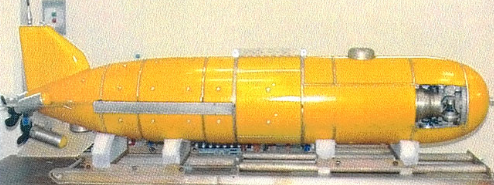
\includegraphics[width=0.7\linewidth]{MTT3000.png}%
	\caption{Автономный необитаемый подводный аппарат ММТ-3000}
	\label{MTT3000}
\end{figure}

Стоит отметить, что у Института Проблем Морских Технологий ДВО РАН огромный опыт по разработке водных роботов, существует множество работ, в которых описаны конструкции разработанных аппаратов, системы управления для них, рассмотрены задачи практического применения~\cite{Inzarcev_2018_book, Matvienko_2017, Naumov_2011, Boreyko_2011, Iznarcev_2007, Vaulin_2017, Inzarcev_2016}.

В работе~\cite{Pshihopov_2014} рассмотрена интеллектуальная система управления автономным подводным аппаратом. Планирование и управление движением построено на иерархической структуре. Подсистема планирования движения основана на нейросети и позволяет определять и обходить препятствия на пути движения робота. Система управления позволяет двигаться вдоль заданной траектории из точки в точку с заданной скоростью. В работе приводятся результаты моделирования системы управления. В качестве объекта моделирования выбран подводный аппарат, который приводится в движение гребным винтом и двумя подруливающими устройствами: горизонтальным и вертикальным. При этом гребной винт может менять свою ориентацию на некоторый угол в горизонтальной и вертикальной плоскости. Для моделирования движения необходимые коэффициенты, такие как положение центра масс и компоненты тензора инерции аппарата вычислены в пакете SolidWorks, гидродинамические характеристики расчитаны в программных комплексах FineHexa и STAR CD, присоединенные массы расчитаны по эмпирическим зависимостям в приближении формы аппарата эллипсоидом. В результате моделирования было показано, что интеллектуальная система управления позволяет избегать столкновений с подвижными и неподвижными препятствиями и способна выполнять поставленные задачи по движению робота по заданной траектории. На практике данная система управления реализована на базе автономного надводного катера, и, в процессе испытаний, показала свою работоспособность при движении из одной точки в другую.



\section{Перемещение за счет изменения формы тела}\label{sec:ch1/sec3}

Несмотря на то, что в разработке и исследовании движения кораблей и подводных лодок, перемещающихся за счет гребных винтов, достигнуты значительные успехи, в настоящее время возник интерес к небольшим водным мобильным роботам, передвигающимся как автономно, так и под управлением оператора. Движение в жидкости данные роботы могут осуществлять как за счет гребных винтов, так и за счет других, нетрадиционных способов. Одним из таких способов является перемещение за счет изменения формы тела.

Перемещение роботов за счет изменения формы тела в основном описывает способы движения плавающих живых существ. Самый распространенный способ --- имитация движений плавников рыб. Вопросы самопродвижения рыб рассматривал еще Аристотель в некоторых своих работах. Существенный прогресс в описании движения подобных деформируемых тел достигнут в конце XIX -- начале XX века~\cite{Alexander_1983}. 

Существует множество способов перемещения за счет изменения формы тела. Только у рыб приводится около 15 различных способов передвижения определяемых движениями тела и плавников~\cite{Blake_1983}. Несмотря на различные способы передвижения, основным фактором влияющим на самопродвижение является вязкость жидкости и связанные с ней процессы вихреобразования. При этом, вязкость, как и сила трения при движении по твердой поверхности, оказывает негативное влияние, вызывая силу вязкого сопротивления, но, с другой стороны, образующиеся вихри продвижению помогают, создавая тяговую силу~\cite{Vetchanin_Kilin_2016}.

Рассмотрим несколько примеров разработанных конструкций роботов имеющих бионические принципы движения.

В работе~\cite{Zheng_2010} разработан робот рыбоподобной формы (см. рисунок~\ref{ZhengRobot}). Робот приводится в движение периодическими колебаниями хвостового плавника, который состоит из пластины, сделанной из полимерного композитного материала, к которой прикреплен пассивный пластиковый плавник. Робот имеет размеры 20 см в длину и около 5.7 см в диаметре не учитывая длину хвостового плавника. Масса робота --- 290 грамм. В работе записаны динамические уравнения движения, которые основаны на работах Дж. Лайтхилла, описавшего механику плавания рыб~\cite{Lighthill_1970}. Проведены экспериментальные исследования по определению коэффициентов сопротивления жидкости, эксперименты с движением в жидкости с пассивным плавником и без него и эксперименты с движением в жидкости с хвостовыми плавниками разных размеров. Представлены графики зависимости скорости движения от частоты колебания плавника для хвостовых плавников различных размеров. Экспериментальные значения довольно хорошо согласуются со значениями, расчитанными по математической модели.

\begin{figure}[h]
	\centering
	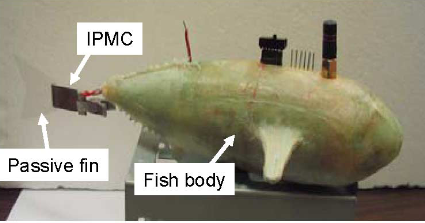
\includegraphics[width=0.7\linewidth]{ZhengRobot.png}%
	\caption{Робот рыбоподобной формы с хвостовым плавником в качестве движителя}
	\label{ZhengRobot}
\end{figure}

В работе~\cite{Wang_Tan} рассмотрен рыбоподобный робот, перемещающийся за счет периодического движения хвостового плавника (см. рисунок~\ref{WangRobot}). В прототипе робота хвостовой плавник изготовлен из углеволокна, который приводится в движение сервоприводом модели HS-5085MG фирмы Hitec. Плавник представляет собой пластину длиной 8 см, шириной 2.5 см и толщиной 1.1 мм. Движением сервопривода управляет микроконтроллер. В работе представлена модель движения, в основе которой лежит  динамика твердого тела и теория Лайтхилла, математически описывающая движение рыб~\cite{Lighthill_1970}. Основные уравнения движения записаны в виде уравнений Кирхгоффа для движения твердого тела в идеальной жидкости~\cite{Kirchhoff}, а теория Лайтхилла позволяет расчитать гидродинамические силы, действующие на подвижный хвостовой плавник. Проведены экспериментальные исследования по движению робота по окружности в бассейне при различном смещении начального угла хвостового плавника, а также с различной частотой колебания и амплитудой. При этом коэффициенты вязкого сопротивления и подъемной силы были аппроксимированы по модели используя экспериментальные данные при движении по окружности с параметрами начального смещения хвостового плавника в 20$^\circ$, частотой колебания $1.8\pi$ рад/с и амплитудой 15$^\circ$. Приведены графики, на которых сравниваются результаты моделирования и экспериментов. Далее получена зависимость коэффициентов вязкого сопротивления от начального смещения хвостового плавника, учитывая эти зависимости, отклонение полученных значений предыдущих экспериментов от расчетных уменьшилось. Затем проведены экспериментальные исследования движения робота по прямой. Модель с адаптированными коэффициентами вязкого сопротивления показывает также лучшее согласование с экспериментом чем модель с постоянными коэффициентами вязкого сопротивления.

\begin{figure}[h]
	\centering
	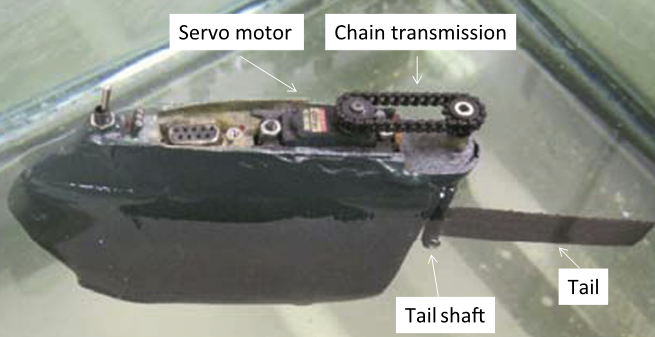
\includegraphics[width=0.7\linewidth]{WangRobot.png}%
	\caption{Рыбоподобный робот, перемещающийся за счет периодического движения хвостового плавника}
	\label{WangRobot}
\end{figure}

В работе~\cite{Zhou_2011} рассматривается мобильный водный робот движущийся в воде за счет колебаний боковых плавников (см. рисунок~\ref{ZhouRobot}). Такой способ управления имитирует движение ската. Робот имеет размеры 500 х 105 х 960 мм и массу 7.3 кг. Скорость движения робота 0.4 м/с. Плавники приводятся в движение сервоприводами по три на каждый плавник. Плавники изготовлены из эластичного резинового материала, по которому идут жесткие ребра от каждого сервопривода. Глубина погружения контролируется датчиком давления и изменяется с помощью двунаправленного насоса, который может набирать воду во внутреннюю полость робота. Законы управления роботом основаны на модели нелинейного осцилятора Хопфа. В экспериментальных исследований представлены движения по прямой с поворотом. %В будущем планируется ввести обратные связи для повышения эффективности управления.

\begin{figure}[h]
	\centering
	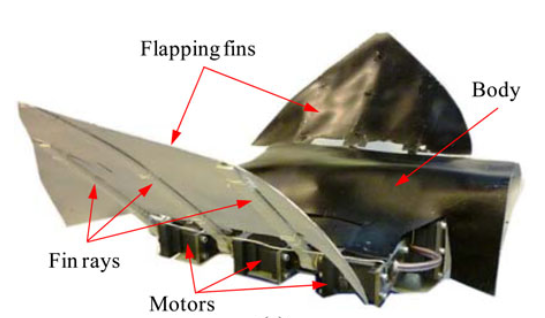
\includegraphics[width=0.7\linewidth]{ZhouRobot.png}%
	\caption{Мобильный водный робот, имитирующий движение ската}
	\label{ZhouRobot}
\end{figure}

\section{Перемещение за счет реактивной тяги}\label{sec:ch1/sec4}

Существуют конструкции, которые реализуют перемещение в жидкости реактивным методом. Движущая сила создается потоком воды, выталкиваемом из движителя, который, в основном, состоит из трубопровода, винта (насоса) и реверсивно-рулевого устройства. Данный тип движителя применялся на речных судах начиная с 50-х годов XX века. В настоящее время реактивные движителя применяются в небольших судах, плавающих на мелководье, начиная от моторных лодок и до скоростных судов.

В мобильной робототехнике реактивный тип движителя встречается нечасто. В качестве примера можно рассмотреть работу~\cite{Lin_2011}, в которой описан подводный робот сферической формы с водометными движителями (см. рисунок~\ref{LinRobot}). Робот имеет три реактивных движителя расположенные под углом 120$ ^\circ $ друг к другу. Каждый движитель имеет 2 степени свободы и может изменять направление выбрасываемой струи в горизонтальной и вертикальной плоскости. Проведены экспериментальные исследования, которые подтвердили возможность движения, используя простые маневры: движение в горизонтальной и вертикальной плоскостях, вращение вокруг вертикальной оси.

\begin{figure}[h]
	\centering
	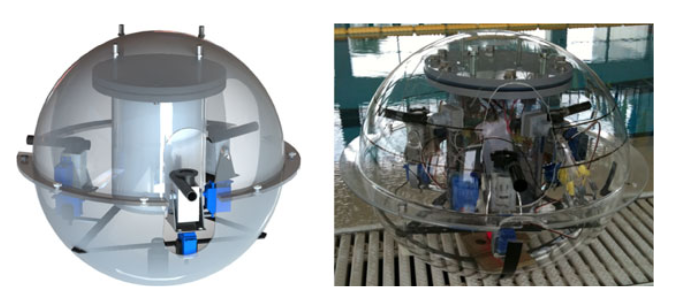
\includegraphics[width=0.7\linewidth]{LinRobot.png}%
	\caption{Подводный сфероробот с реактивными движителями}
	\label{LinRobot}
\end{figure}

\section{Перемещение за счет внутренних механизмов}\label{sec:ch1/sec5}

Устройства, перемещающиеся за счет движения внутренних масс так же представляют интерес. Можно подобрать необходимые характеристики движения внутренних масс для движения мобильного робота в заданном направлении. Отсутствие внешних подвижных элементов является главным преимуществом таких систем, так как воздействие на окружающую среду оказывается минимальное. Для исследования подобных объектов необходима математическая модель движения, которая позволяет определить основные параметры и характеристики прототипа мобильного робота, а также необходимые условия для проведения экспериментов.

Для описания управляемого движения твердых тел в жидкости предложены различные математические модели. Наиболее простые модели построены в рамках теории идеальной жидкости и учитывают только эффект присоединенных масс. Однако такие существенно упрощенные модели позволяют обнаружить интересные динамические эффекты и закономерности, наблюдаемые в экспериментах. Например, в работах \cite{Kozlov_Ramodanov_PMM_2001, Kozlov_Onichenko} рассматривалось продвижение твердых тел в идеальной жидкости за счет подвижных внутренних масс. Показано, что неограниченное продвижение оказывается возможным только при наличии анизотропии присоединенных масс. Идеи работ \cite{Kozlov_Ramodanov_PMM_2001, Kozlov_Onichenko} получили развитие в \cite{Vetchanin_Kilin_2016}, где рассматривалось движение эллиптического профиля, содержащего два эксцентрика, вращающихся с одинаковыми по модулю и противоположными по знаку скоростями. Показано, что такая система движется в среднем прямолинейно. Данный факт подтверждается экспериментально, см. \cite{Klenov_Kilin_2016}. Также можно отметить работу \cite{Jing_Kanso_2013}, где рассматривалась задача устойчивости движения эллиптического профиля за счет вращательных колебаний. Трехмерные задачи управления и стабилизации движения эллипсоидов и винтовых тел рассматривались, например, в работах \cite{Borisov_et_al_2017, Vetchanin_Mamaev_2017, Vetchanin_et_al_2016, Woolsey_Leonard_1999}.

Модель схода вихрей позволяет описать самопродвижение тела за счет колебаний внутреннего ротора, наблюдаемое в экспериментах \cite{Tallapragada_2015, Pollard_Tallapragada_2019}. Однако, следует отметить, что сход каждого вихря приводит к увеличению размерности фазового пространства системы, что влечет определенные вычислительные трудности. Альтернативой описанной модели являются конечномерные математические модели, учитывающие вязкое трение и изменение циркуляции. Например, в работе \cite{Borisov_et_al_2018} рассматривалось плоскопараллельное движение эллиптического профиля за счет колеблющегося ротора при наличии периодически изменяющейся циркуляции и вязкого трения. Подобная модель для тела с острой кромкой и циркуляцией, изменяющейся согласно условию Кутты-Чаплыгина, предложена в работе \cite{Mamaev_Vetchanin_2018} на основе результатов численных экспериментов, описанных в работе \cite{Mamaev_et_al_2018}. В работе \cite{Kilin_et_al_2018} предложена модель движения робота с двумя эксцентриками, учитывающая помимо вязкого сопротивления, качку во время движения.

Отметим, что наиболее полное описание движения тел в жидкости может быть получено на основе совместного решения уравнений движения тела и уравнений Навье-Стокса, см., например, работы \cite{Childress_et_al_2011, Eldredge_2006, Vetchanin_et_al_2013}. Однако использование такого подхода затратно с вычислительной точки зрения при исследовании управляемого движения и построении гейтов. Поэтому моделирование с использованием уравнений Навье-Стокса целесообразно только при построении конечномерных моделей движения тел в жидкости, которые оказываются более удобными при анализе управляемого движения.

Рассмотрим более подробно некоторые работы.

В работе \cite{Volkova_Jatsun} рассматривается робот, состоящий из корпуса, двух подвижных внутренних масс и четырех поплавков. Движение робота осуществляется за счет перемещения подвижных масс относительно корпуса по прямолинейным направляющим (см. рисунок~\ref{JatsunRobot}). Робот держится на поверхности жидкости за счет четырех опорных поплавков с изменяемым углом наклона относительно вертикали. Изменение положения поплавков позволяет изменять силы трения вдоль продольной оси корпуса во время движения. В работе описана математическая модель движения и проведено численное моделирование, позволившее изучить управляемые движения робота на примере прямолинейного и вращательного движения.

\begin{figure}[h]
	\centering
	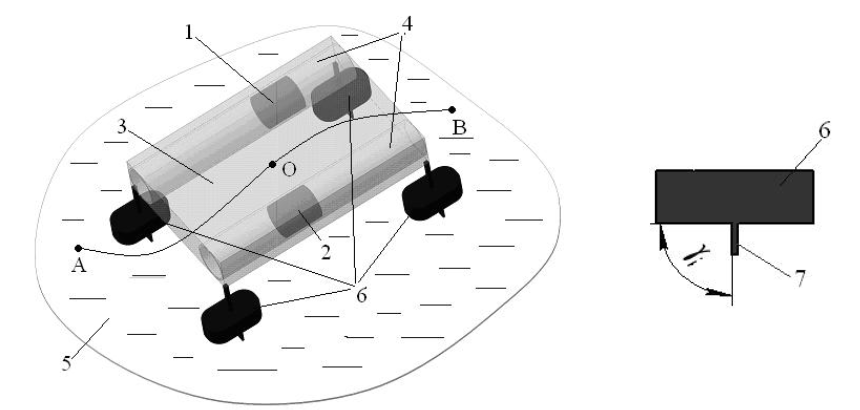
\includegraphics[width=0.7\linewidth]{JatsunRobot.png}%
	\caption{Схематичное изображение плавающего робота и схема поплавка}
	\label{JatsunRobot}
\end{figure}

В диссертации~\cite{Klenov_diss} и в работе~\cite{Klenov_Kilin_2016} рассмотрена локомоционная мобильная платформа, перемещающаяся в жидкости за счет изменения распределения масс (см. рисунок~\ref{TolikRobot}). Разработана математическая модель плоскопараллельного движения в рамках модели идеальной жидкости и математическая модель движения с учетом внешних сил, действующих на объект со стороны жидкости на основе уравнений Кирхгоффа~\cite{Kirchhoff}. Первая математическая модель показала качественное согласование результатов моделирования и экспериментов, тогда как вторая, уточненная модель движения, позволила достичь количественного согласования. Описана конструкция изготовленного натурного образца~\cite{patent_BNR}, который движется по поверхности жидкости. Проведены и описаны экспериментальные исследования. Работа с безвинтовым подводным роботом с внутренними роторами в данной диссертации является продолжением вышеописанных исследований. Так как математическая модель, разработанная в рамках модели идеальной жидкости, имела качественное согласование с экспериментами, для безвинтового подводного робота разработана подобная модель, которая описывает трехмерное движение.

\begin{figure}[h]
	\centering
	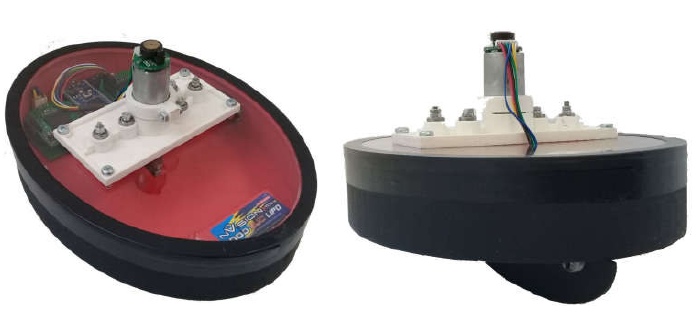
\includegraphics[width=0.7\linewidth]{TolikRobot.png}%
	\caption{Локомоционная мобильная платформа, перемещающаяся в жидкости за счет изменения распределения масс}
	\label{TolikRobot}
\end{figure}

В работе~\cite{Pollard_Tallapragada_2016} рассмотрен водный робот, имеющий форму профиля крыла NACA 0030 (см. рисунок~\ref{TallapragadaRobot}). Робот перемещается в жидкости за счет периодического вращения внутреннего ротора. Разработана математическая модель движения, учитывающая сход вихрей с острой кромки. В качестве функции управления скоростью вращения ротора рассматривается прямоугольный сигнал, чего на практике быть не может, так как для разгона ротора с большим моментом инерции до определенной скорости необходимо некоторое время. В работе довольно подробно исследовано движение вдоль прямой. Так же рассматривается такой маневр, как разворот на 180$^\circ$. Для этого управляющее воздействие делится на 3 участка: управление для движения по прямой, управления для разворота, снова управление для движения по прямой. Таким образом удалось добиться разворота на 180$^\circ$ по траектории с радиусом 750 мм. Следует отметить, что для выполнения разворота, в управляющем воздействии изменяется значения скорости вращения ротора в одном и направлений, что не является верным.

\begin{figure}[h]
	\centering
	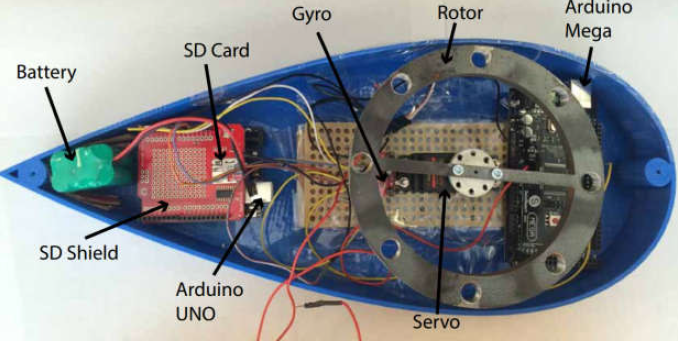
\includegraphics[width=0.7\linewidth]{TallapragadaRobot.png}%
	\caption{Водный робот, имеющий форму профиля крыла NACA 0030}
	\label{TallapragadaRobot}
\end{figure}

В работе~\cite{Pollard_Tallapragada_2019} авторы продолжают исследовать динамику водного робота с формой профиля крыла NACA 0030. Здесь проведено сравнение маневренности вышеописанного робота при различных вариантах исполнения хвостовой части корпуса: полностью жесткий корпус, корпус со свободно вращающейся однозвенной хвостовой частью и два варианта корпуса со свободно вращающейся двухзвенной хвостовой частью (см. рисунок~\ref{TallapragadaRobot2}). Маневренность оценивалась выполнением робота разворота на 180$^\circ$ из состояния покоя и после движения по прямой. При этом управление для разворота задавалось вращением ротора с постоянной максимально возможной для данной конструкции скоростью в одном направлении. При таком управляющем воздействии робот с полностью жестким корпусом на данный угол повернуть не смог, из состояния покоя робот повернул на 155$^\circ$, а поворот после движения по прямой составил 110$^\circ$. Варианты исполнения корпуса с подвижной хвостовой частью оказались более маневренными. Наилучшего результата удалось добиться для варианта корпуса с двухзвенной хвостовой частью: поворот на 180$^\circ$ осуществлен за 4.1 секунда с радиусов поворота порядка 200 мм. Здесь следует отметить, что такое управляющее воздействие для поворота, либо движения по траектории с некоторым радиусом, является не самым эффективным. Ниже в данной диссертации будут рассмотрены эксперименты с движением робота подобной формы с полностью жестким корпусом, приведены управляющие воздействия при которых робот движется по траектории в виде окружности с минимальным радиусом 185 мм.

\begin{figure}[h]
	\centering
	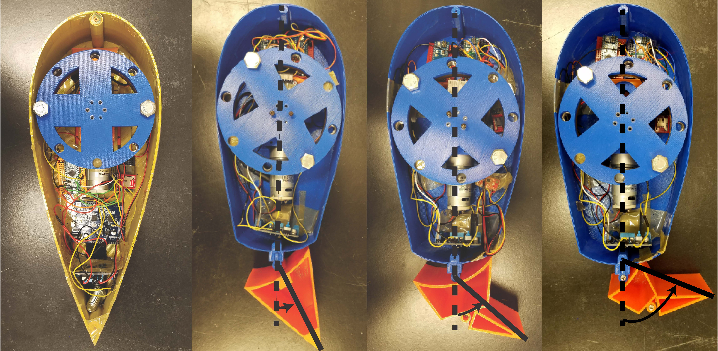
\includegraphics[width=0.7\linewidth]{TallapragadaRobot2.png}%
	\caption{Варианты исполнения водного робота со свободно вращающимся хвостом}
	\label{TallapragadaRobot2}
\end{figure}



В работе \cite{Ramodanov_Tenenev} рассматривается задача о движении тела в вязкой жидкости, за счет перемещения внутренних масс, при котором внешняя оболочка тела остается неизменной. Приведена математическая модель, основанная на уравнениях динамики твердого теоа и гидродинамических уравнениях Навье-Стокса. В результате численного моделирования показано существенное влияние сил и момента вязкого сопротивления на траекторию движения, выявлены отличия движения тела в вязкой жидкости по сравнению с идеальной. На основе полученных результатов в работе \cite{Vetchanin_Tenenev_2011} решена задача оптимального управления движением тела по заданной траектории за счет перемещения внутренних масс, с применением гибридного генетического алгоритма. В результате получены аппроксимационные зависимости для сил, действующих на тело.

Исследование характеристик движения тела с переменным распределением массы в трехмерной постановке в вязкой жидкости проведено в работе \cite{Vetchanin_Mamaev_Tenenev_ND_2012}, а в работе \cite{Vetchanin_Kilin_2017} рассмотрено управляемое движение при наличии циркуляции вокруг тела. В этих работах показана возможность перемещения тела в произвольном направлении, а также возможность преодоления силы тяжести телом с плавучестью близкой к нулевой.

\section{Выводы по главе}

В данной главе рассмотрен подход к построению математических моделей движения объектов в жидкости, приведен обзор различных способов перемещения в жидкости, для каждого способа перемещения рассмотрены несколько экспериментальных работ. Из обзора было выявлено, что самым распространенным движителем в жидкости является гребной винт. Но также существует интерес к бионическим способам приведения в движение и движению за счет внутренних механизмов. На данный момент движение за счет внутренних механизмов является малоизученным, но при этом существуют задачи, в которых роботы, использующие этот способ перемещения, могут иметь преимущество перед роботами с гребными винтами.

Данная работа является продолжением исследований описанных в работах~\cite{Klenov_diss, Klenov_Kilin_2016}, в которых изучается динамика робота, перемещающегося по поверхности жидкости за счет периодического смещения центра масс системы. Используя математическую модель, построенную в рамках модели идеальной жидкости, удалось получить траектории движения, которые качественно согласуются с экспериментальными траекториями. В следующей главе рассмотрим подобную математическую модель для трехмерного движения мобильного робота. Следует отметить, что при движении в толще жидкости удобнее управлять объектом, у которого центр масс системы не изменяется и находится в центре давления, поэтому принято решение в качестве управления использовать вращение роторов, а не эксцентриков, как в~\cite{Klenov_diss, Klenov_Kilin_2016}. Подобный способ управления был описан для шара, движущегося на плоскости~\cite{BKM_Chapligin1, BKM_Chapligin2}.



           % Глава 1
\chapter{Математическая модель движения мобильных плавающих роботов}\label{ch:ch2}

\section{Описание математчиеской модели движения мобильного робота в форме эллипсоида в жидкости}\label{sec:ch2/sec1}

Рассмотрим систему, состоящую из жесткой внешней оболочки и трех внутренних роторов (рисунок \ref{rotors}). Геометрический центр системы совпадает с центром сферической части оболочки.

\begin{figure}[th]
	\begin{center}
		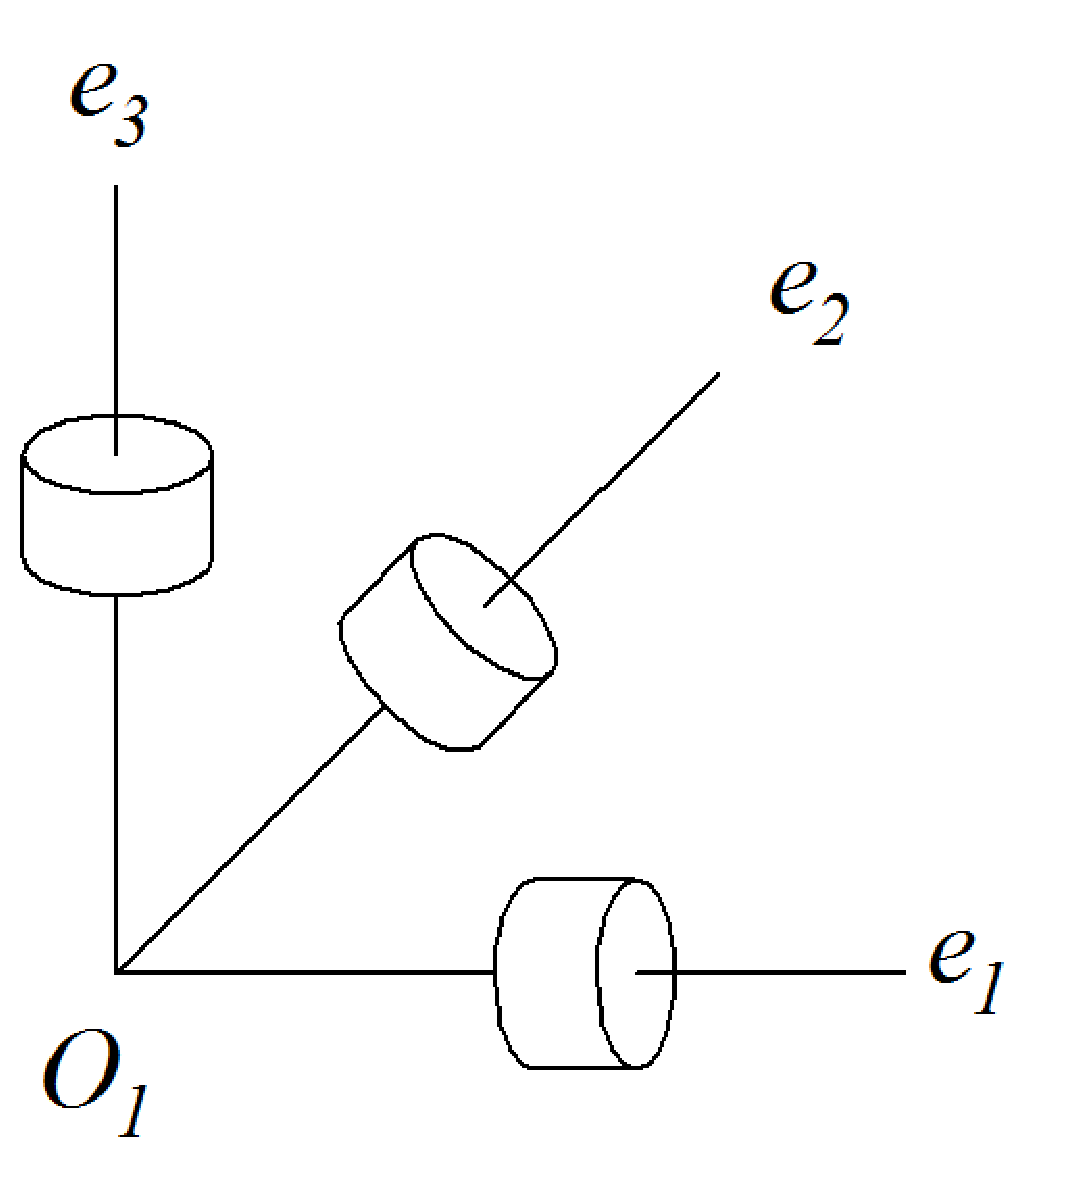
\includegraphics[width=0.3\linewidth]{rotors1.eps}
		\caption{Расположение роторов} \label{rotors}
	\end{center}
\end{figure}


Будем полагать, что конструкция удовлетворяет ряду условий:
\begin{enumerate}
	\item Оболочка является однородной, положение ее центра масс совпадает с геометрическим центром оболочки.
	%\item Центр масс всей системы находится не в геометрическом центре оболочки;
	\item Все роторы одинаковы, осесимметричны и оси вращения  совпадают с их осями симметрии, то есть вращение не изменяет распределение масс системы;
	%\item Ось вращения одного из роторов совпадает с осью винтовой симметрии оболочки;
	\item Оси вращения роторов взаимно перпендикулярны, а их угловые скорости являюся заданными функциями времени $\omega _k \bigl( t \bigr),~k=1,2,3$.
\end{enumerate}

Выберем подвижную систему координат $O_1 e_1 e_2 e_3$, жестко связанную с оболочкой, так что оси совпадают с главными осями инерции оболочки. Обозначим через $\bV$ и ${\bOm}$ скорость центра оболочки и его угловую скорость (все векторы, если не оговорено обратное, проецируются на подвижные оси).

Определим дополнительно неподвижную систему координат $O x y z$ и обозначим $\br = \bigl( x,\, y,\, z \bigr)$ -- координаты геометрического центра оболочки в этих осях. Обозначим также через ${\bal}$, ${\bbe}$, ${\bga}$ орты неподвижных осей $O x y z$, спроецированные на подвижные оси $e_1$, $e_2$, $e_3$, тогда ортогональная матрица
\begin{gather}
\bbQ =\begin{pmatrix}
\alpha _1 & \beta _1 & \gamma _1\\
\alpha _2 & \beta _2 & \gamma _2\\
\alpha _3 & \beta _3 & \gamma _3
\end{pmatrix}\nonumber \in SO(3)
\end{gather}

характеризует ориентацию тела, а пара $\left( \br,\, \bm{Q} \right)$ однозначно определяет конфигурацию системы. Таким образом, конфигурационное пространство системы шестимерно и представляет собой $\mathbb{R}^3 \times SO(3)$.

Обозначим через $m_s$ -- массу оболочки, ${\bm I}_s$ -- ее центральный тензор инерции,
\begin{gather}
\bLam = \begin{pmatrix}
\bLam _1 & 0 \\
0 & \bLam _2
\end{pmatrix}\nonumber
\end{gather}
-- матрицу коэффициентов присоединенных масс в системе $O e_1 e_2 e_3$, где $\bLam_1$ -- тензор присоединенных масс, $\bLam_2$ -- тензор присоединных моментов инерции. Тогда выражение для кинетической энергии оболочки примет вид
\begin{gather}
T_s = \frac{1}{2} m_s  \bigl( \bV,\, \bV \bigr) + \frac{1}{2} \bigl( {\bm I}_s {\bOm},\, {\bOm} \bigr),\nonumber
\end{gather}
а выражение кинетической энергии жидкости
\begin{gather}
T_f = \frac{1}{2} \bigl( \bLam_1 \bV,\, \bV \bigr) + \frac{1}{2} \bigl( {\bLam} _2 {\bOm},\, {\bOm} \bigr).\nonumber
\end{gather}

Обозначим через $m_R$ -- массу ротора, ${\bbI}_k$ -- центральный тензор инерции $k$-го ротора, записанный в системе координат $O' e_1 e_2 e_3$, $\bn_k$ -- орт оси вращения $k$-го ротора неподвижный в системе $O' e_1 e_2 e_3$, $\br_k$ -- радиус-вектор центра масс $k$-го ротора неподвижный в системе $O' e_1 e_2 e_3$. Тогда кинетическая энергия $k$-го ротора примет вид
\begin{gather}
T_k = \frac{1}{2} m_R \bigl( \bV + {\bOm} \times \br_k, \bV + {\bOm} \times \br_k \bigr) + \frac{1}{2}\Bigl({\bm I}_k \bigl( {\bOm} + \omega_k \bn_k \bigr), {\bOm} + \omega_k \bn_k \Bigr),\nonumber
\end{gather}

Суммарная кинетическая энергия всей системы с учетом того, что оси роторов задаются собственными векторами их тензоров инерции, то есть ${\bbI}_k \bn_k = i \bn_k$, примет вид
\begin{gather}
\label{kinetic_energy}
\begin{split}
T = & T_f + T_s + \sum _{k=1}^3 T_k = \\
= & \frac{1}{2} \bigl( {\bbI} {\bOm},\, {\bOm} \bigr) + \bigl( {\bbB} {\bOm},\, \bV \bigr) + \frac{1}{2} \bigl( {\bbC} \bV,\, \bV \bigr) + \bigl( {\bOm},\, \bK(t) \bigr) + \frac{1}{2} \sum_{k=1}^3 i \omega_k^2 (t),
\end{split}
\end{gather}
где $\bbI$ --- тензор инерции всей системы вычисленный относительно геометрического центра оболочки, матрицы $\bbB$ и $\bbC$ зависят от распределения масс и формы оболочки, $\bK(t)=\sum \limits_{k=0}^3 i \omega_k (t)\bn_k$ --- вектор гиростатического момента. Матрицы $\bbI$, $\bbB$, $\bbC$ имеют вид
\begin{gather}
{\bbI} = {\bLam}_2 + {\bbI}_s + \sum _{k=1}^3 {\bbI}_k + \frac{1}{2} m_R \sum _{k=1}^3 \bigl( \br_k^2{\bbE} - \br_k \otimes \br_k \bigr),\nonumber \\
{\bbC} = m {\bbE} + {\bLam}_1,\nonumber \\
{\bbB} = m \begin{pmatrix}\nonumber
0 & z_c & -y_c\\
-z_c & 0 & x_c\\
y_c & -x_c & 0
\end{pmatrix}\nonumber \\
m = m_s + 3 m_R,\nonumber
\end{gather}
где $x_c$, $y_c$, $z_c$ --- компоненты радиус-вектора $\br_c$ центра масс системы.

\begin{small}
	{\textbf{ Замечание.} Общее число параметров матриц $\bbC$, $\bbB$, $\bbI$ равно 21. С помощью подходящего выбора точки $O_1$ и ориентации осей $O_1 e_1 e_2 e_3$ матрицу $\bbI$ можно привести к диагональному виду, $\bbB$ -- к симметрическому, а общее число параметров будет равно 15 \cite{Borisov_Mamaev}. Исследования, которые будут проводиться в дальнейшем, будут осуществляться численно, поэтому вопрос о количестве параметров не является принципиальным.}
\end{small}

Уравнения движения рассматриваемой системы имеют вид классических уравнений Кирхгофа \cite{Borisov_Mamaev}
\begin{gather}
\label{Kirchhoff}
\frac{d}{dt} \biggl( \frac{\partial T}{\partial \bV} \biggr) + {\bOm} \times \frac{\partial T}{\partial \bV}=0, \quad \frac{d}{dt}\biggl( \frac{\partial T}{\partial {\bOm}} \biggr) + {\bOm} \times \frac{\partial T}{\partial {\bOm}} + \bV \times \frac{\partial T}{\partial \bV} = 0 \nonumber
\end{gather}
и с учетом (\ref{kinetic_energy}) могут быть записаны в виде
\begin{gather}
\label{motion_eq}
\begin{split}
{\bbC} \dot{\bV} + {\bbB} \dot{{\bOm}} = & \bigl( {\bbC} \bV + {\bbB} {\bOm} \bigr) \times {\bOm},\\
{\bbB}^T \dot{\bV} + {\bbI} \dot{{\bOm}} + \dot{\bK}(t) = & \bigl( {\bbB}^T \bV + {\bbI} {\bOm} + \bK(t) \bigr) \times {\bOm} + \bigl( {\bbC} \bV + {\bbB} {\bOm} \bigr) \times \bV = 0
\end{split}
\end{gather}

Данные уравнения необходимо дополнить уравнениями эволюции переменных $\bigl( \br,\, {\bbQ} \bigr)$, которые описываются уравнениями Пуассона и кинематическими соотношениями следующего вида
\begin{gather}
\label{kinematics_abg}
\dot{{\bal}} = {\bal} \times {\bOm},\, \dot{{\bbe}} = {\bbe} \times {\bOm},\, \dot{{\bga}} = {\bga} \times {\bOm},\\
\dot{\br} = {\bbQ}^T \bV.\label{kinematics_r}
\end{gather}

Уравнения \eqref{motion_eq}, \eqref{kinematics_abg}, \eqref{kinematics_r} полностью описывают движение рассматриваемой системы. Однако удобней записать данные уравнения в гамильтоновой форме \cite{Clebsch}
\begin{gather}
\label{motion_ham}
\dot{\bP}= \bP \times {\bOm},\,\dot{\bM} = \bM \times {\bOm} + \bP \times \bV,
\end{gather}
где $\bP = \dfrac{\partial T}{\partial \bV}$ и $\bM = \dfrac{\partial T}{\partial {\bOm}}$ имеют гидродинамический смысл и называются, соответственно, импульсивным моментом и импульсивной силой. При этом $\bV$ и ${\bOm}$ связаны с этими векторами следующим образом
\begin{gather}
\label{p_and_M}
\begin{split}
\bP = & {\bbC} \bV + {\bbB} {\bOm},\, \bM = {\bbB}^T \bV + {\bbI} {\bOm} + \bK(t),\\
\bV = & {\bbC}^{-1} \bigl( \bP - {\bbB} {\bOm} \bigr),\, {\bOm} = \bigl({\bbI} - {\bbB}^T {\bbC}^{-1} {\bbB} \bigr)^{-1} \bigl( \bM - \bK(t) - {\bbB}^T {\bbC}^{-1} \bP \bigr)
\end{split}\nonumber
\end{gather}

Уравнения \eqref{motion_ham} являются гамильтоновыми на алгебре $e(3)$ с гамильтонианом
\begin{gather}
H = \bigl( \bM,\, {\bOm} \bigr) - T \big| _{{\bOm},\, \bV \rightarrow \bM,\, \bP}\nonumber
\end{gather}

Уравнения \eqref{kinematics_abg} допускают шесть геометрических интегралов движения:
\begin{gather}
{\bal}^2={\bbe}^2={\bga}^2=1,\, \bigl({\bal},\, {\bbe} \bigr) = \bigl({\bal},\, {\bga} \bigr) = \bigl({\bbe},\, {\bga} \bigr) = 0\nonumber
\end{gather}

Как указано в \cite{Kozlov_Ramodanov_PMM_2001} уравнения (\ref{motion_ham}) допускают еще шесть интегралов
\begin{gather}
(\bP,\, {\bal}),\, (\bP,\, {\bbe}),\, (\bP,\, {\bga}),\, (\bM + \br \times \bP,\, {\bal}),\, (\bM + \br \times \bP,\, {\bbe}),\, (\bM + \br \times \bP,\, {\bga}) \label{integrals}
\end{gather}

Данные интегралы движения имеют следующий смысл: при движении тела в идеальной жидкости векторы $\bP$ и $\bM + \br \times \bP$ сохраняются в абсолютном пространстве. В случае движения из состояния покоя первые интегралы \eqref{integrals} приобретают особенно простой вид
\begin{gather}
\bP = 0, \quad \bM = 0 \nonumber
\end{gather}
а выражения для скоростей
\begin{gather}
\bV = - \bbC^{-1} \bbB \bOm, \label{v} \nonumber \\
\bOm = - \bigl(\bbI - \bbB^T \bbC^{-1} \bbB \bigr)^{-1} \bK(t) \label{omega} \nonumber
\end{gather}
%\textit{Замечание}. Выражения (\ref{p_and_M}) показывают, что для уравновешенной механической системы (центр масс совпадает с геометрическим центром оболочки)
%
%если механическая система уравновешена, то есть центр масс совпадает с геометрическим центром оболочки, матрица ${\bbB}$ становится нулевой, то перемещение в идеальной жидкости невозможно.

Решения системы уравнений \eqref{motion_eq} и \eqref{kinematics_abg} относительно $\bK(t)$ позволяют находить управляющие воздействия $\omega_k (t)$ для движения вдоль заданной траектории, которая описывается уравнением \eqref{kinematics_r}.



\section{Описание математчиеской модели движения недеформируемого рыбоподобного робота в жидкости}\label{sec:ch2/sec2}

\section{Схема управления мобильными водоплавающими роботами}\label{sec:ch2/sec3}

В полученных математических моделях управление роторами задается в виде вектора внутреннего гиростатического момента $\bK$. Для управления отдельным двигателем разработана следующая схема (см. рисунок \ref{Control_system}).

\begin{figure}[h]
	\centering
	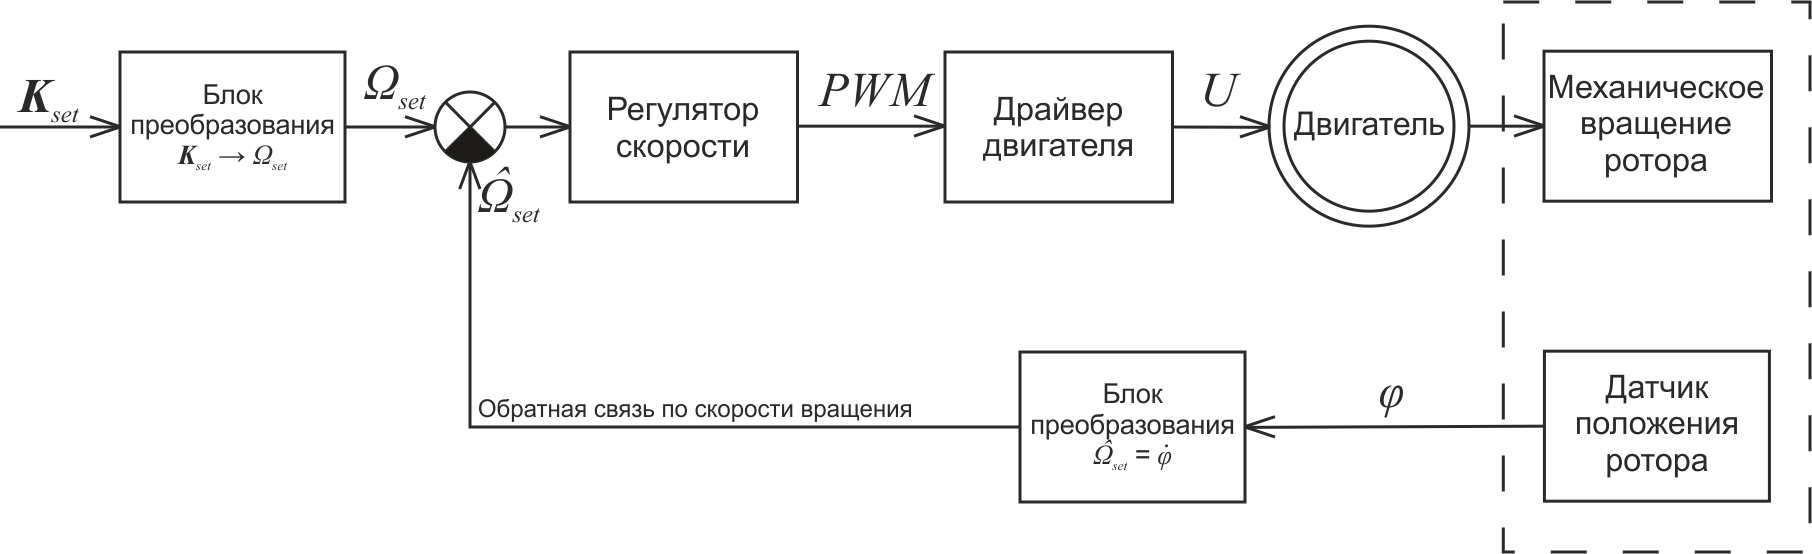
\includegraphics[width=0.9\linewidth]{Control_system.png}%
	\caption{Схема управления отдельным двигателем, где $\bK_{set}$ -- вектор внутреннего гиростатического момента; $\bOm_{set}$ -- угловая скорость вращения двигателя; $\hat{\bOm}_{set}$ -- фактическая скорость вращения двигателя; $PWM$ -- широтно-импульсная модуляция, рассчитаная для заданной скорости вращения; $U$ -- напряжение, подаваемое на двигатель; $\varphi$ -- фактическое положение ротора}
	\label{Control_system}
\end{figure}
           % Глава 2
\chapter{Конструкция безвинтового подводного робота с внутренними роторами}\label{ch:ch3}

Основываясь на математической модели движения, конструкция робота должна соответствовать следующим требованиям:

\begin{itemize}
	\item Перпендикулярность роторов.
	\item Для создания максимального эффекта момент инерции роторов должен быть максимальным.
	\item Центр масс всей системы должен быть расположен максимально близко к геометрическому центру эллипсоида.
\end{itemize}

Для минимального отклонения центра масс от геометрического центра эллипсоида вместо каждого ротора будем использовать пару роторов. В каждой паре роторы должны быть равноудалены от центра эллипсоида и распологаться на осях эллипсоида.

\section{Описание конструкции безвинтового подводного робота с внутренними роторами}

Безвинтовой подводный робот является мобильным роботом в форме эллипсоида и представляет собой сборную конструкцию (рисунок \ref{constr_BPR}). Основой конструкции является оболочка 1 в форме эллипсоида, составленная из двух одинаковых половин 2, присоединенных друг к другу по экваториальной плоскости с помощью дискообразной перегородки – платформы 3. Размер эллипсоида по большей оси составляет 300 мм, по меньшей – 200 мм. Толщина оболочки (3 мм) и применяемый материал обеспечивают необходимую прочность при погружении и перемещении робота. Соединение полуоболочек и платформы обеспечивает герметичность внутренней полости.

\begin{figure}[h]
	\centering
	\includegraphics[width=0.9\linewidth]{constr_BPR.png}%
	\caption{Конструкция и корпусные элементы экспериментальной модели безвинтового подводного робота}
	\label{constr_BPR}
\end{figure}

Размещение узлов на платформе выполнено таким образом, чтобы в максимальной степени обеспечить симметричное расположение масс относительно геометрического центра тела, а также по возможности обеспечить минимальное отклонение центра масс от геометрического.

Внутри корпуса робота установлены три пары роторов (далее система роторов) таким образом, что оси роторов расположены под углом $90^\circ$ по отношению друг к другу. Ось одной из пар роторов направлена вдоль оси вращения эллипсоида, а две другие пары расположены в экваториальной плоскости. Обеспечение точного управляющего воздействия $\omega_k (t)$ осуществляется с помощью встроенных в приводы датчиков обратной связи (энкодеров). Система роторов подводного робота включает пару роторов большего размера 4, установленных симметрично относительно платформы 3 на одной общей оси, и двух других пар роторов меньшего размера 5, расположенных (по направлениям осей) перпендикулярно первой паре и перпендикулярно друг другу в экваториальной плоскости. Оси малых роторов выполнены отдельно для каждого маховика и установлены соосно на некотором расстоянии друг от друга. Малые роторы соединены кинематически попарно с помощью промежуточных (дополнительных) осей и зубчатых пар таким образом, что их вращение происходит также, как если бы они были на одной общей оси.

Характеристики безвинтового подводного робота с внутренними роторами разработанной конструкции представлены в таблице~\ref{tabCharBPR}.
% : масса оболочки: $2.923$ кг; момент инерции маховиков большего размера: $7.491\cdot10^{-4}$ кг$\cdot$м; масса маховиков большего размера: $0.903$ кг;	момент инерции маховиков меньшего размера: $0.491\cdot10-4$ кг$\cdot$м;	масса маховиков меньшего размера: $0.337$ кг.

\begin{table}[h]
	\centering
	\caption{Характеристики безвинтового подводного робота с внутренними роторами}\label{tabCharBPR}
	\begin{tabular}{|l|c|}
		\hline
		Масса оболочки	&	$2.923$ кг 	\\ \hline
		Масса большого ротора &	$0.903$ кг	\\ \hline
		Масса малого ротора &	$0.337$ кг \\ \hline
		Момент инерции большого ротора 	& $7.491\cdot10^{-4}$ кг$\cdot$м \\ \hline
		Момент инерции малого ротора &  $0.491\cdot10-4$ кг$\cdot$м\\ \hline
	\end{tabular}
\end{table}

Фотографии робота в сборе и без половины оболочки представлены на рисунке \ref{Photo_BPR}.

\begin{figure}[h]
	\centering
	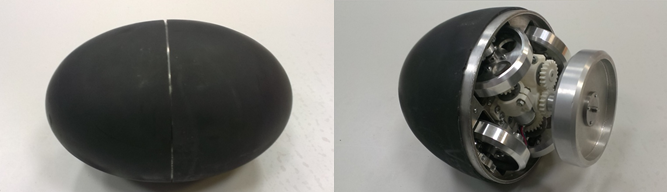
\includegraphics[width=0.9\linewidth]{Photo_BPR.png}%
	\caption{Фотографии безвинтового подводного робота}
	\label{Photo_BPR}
\end{figure}


Для приведения в движение системы роторов каждая из пар роторов оснащена высокомоментными мотор-редукторами, которые установлены в соответствующих опорах на платформе. Кинематическая схема передачи вращения от двигателей к роторам представлена на рисунке~\ref{KinemBPR}.

\begin{figure}[h]
	\centering
	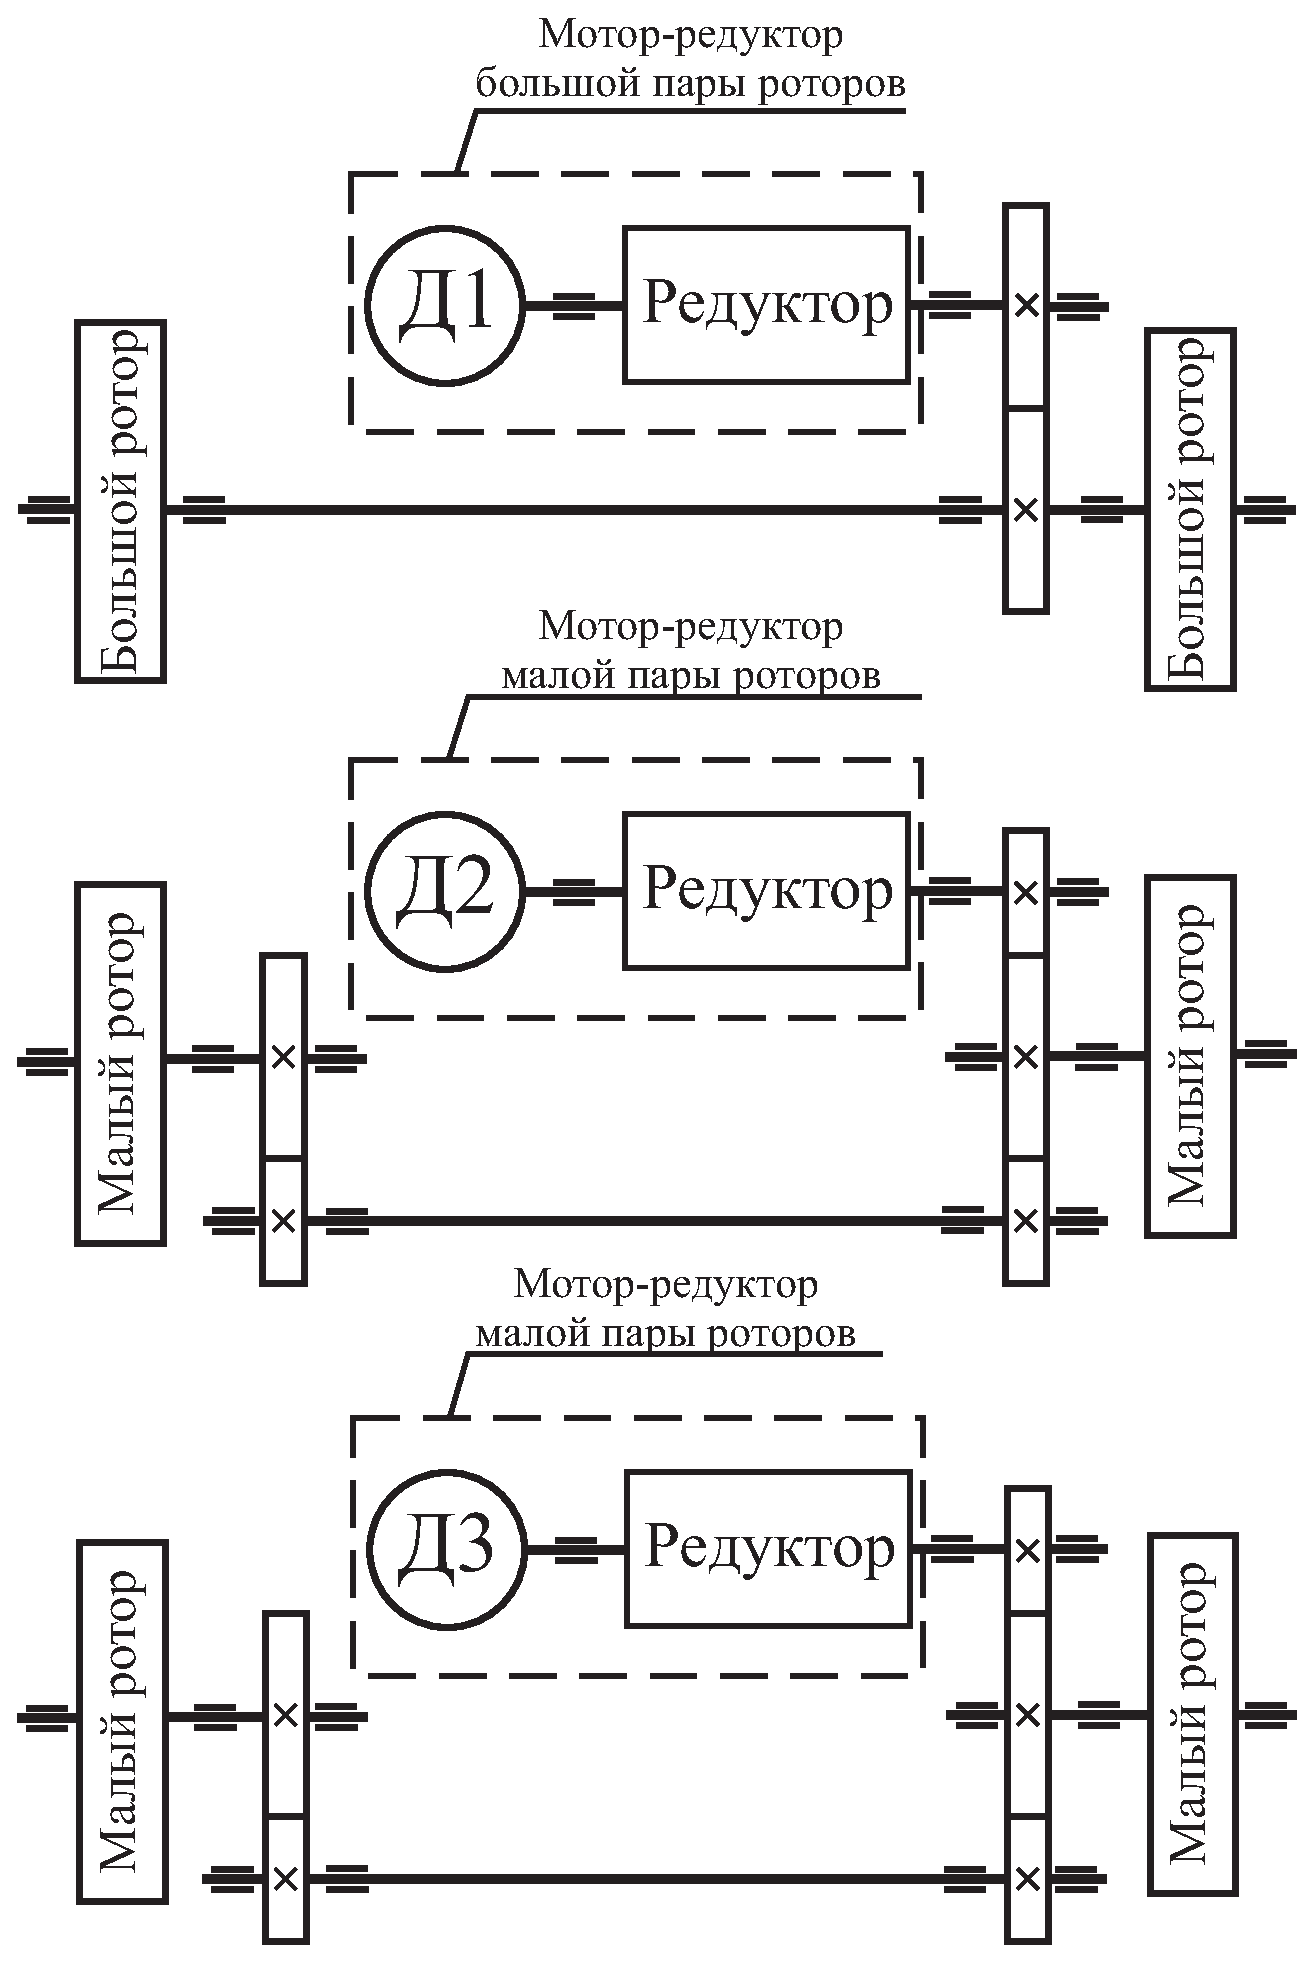
\includegraphics[width=0.6\linewidth]{KinemBPR.eps}%
	\caption{Кинематическая схема передачи вращения от двигателей к роторам}
	\label{KinemBPR}
\end{figure}

В качестве двигателя использовался мотор-редуктор фирмы Pololu с энкодером модели 25D Medium Power (см. рисунок~\ref{MotorBPR}). Характеристики двигателя: номинальное напряжение питания -- 12 В, передаточное отношение редуктора -- 47:1, момент на валу -- 0.6 Нм, максимальная скорость вращения -- 160 об/мин, ток холостого хода -- 200 мА, пусковой ток -- 2.1 А. 

\begin{figure}[h]
	\centering
	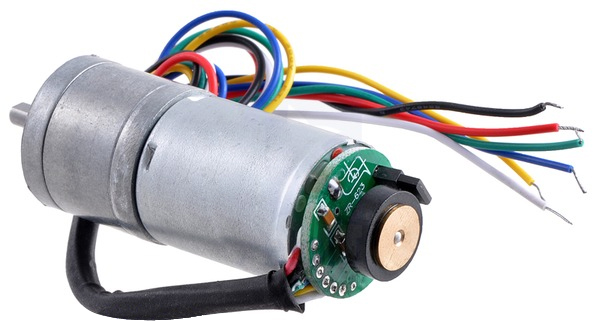
\includegraphics[width=0.5\linewidth]{Motor.jpg}%
	\caption{Мотор-редуктор фирмы Pololu с энкодером модели 25D Medium Power}
	\label{MotorBPR}
\end{figure}





Пара больших роторов расположена на оси, совпадающей с большей осью эллипсоида. Двигатель расположен параллельно этой оси и передача вращения от двигателя к роторам происходит через пару шестерен с 20 зубьями и передаточным отношением 1:1. 3Д-модель данной конструкции представлена на рисунке~\ref{BigRotorsBPR}.

\begin{figure}[h]
	\centering
	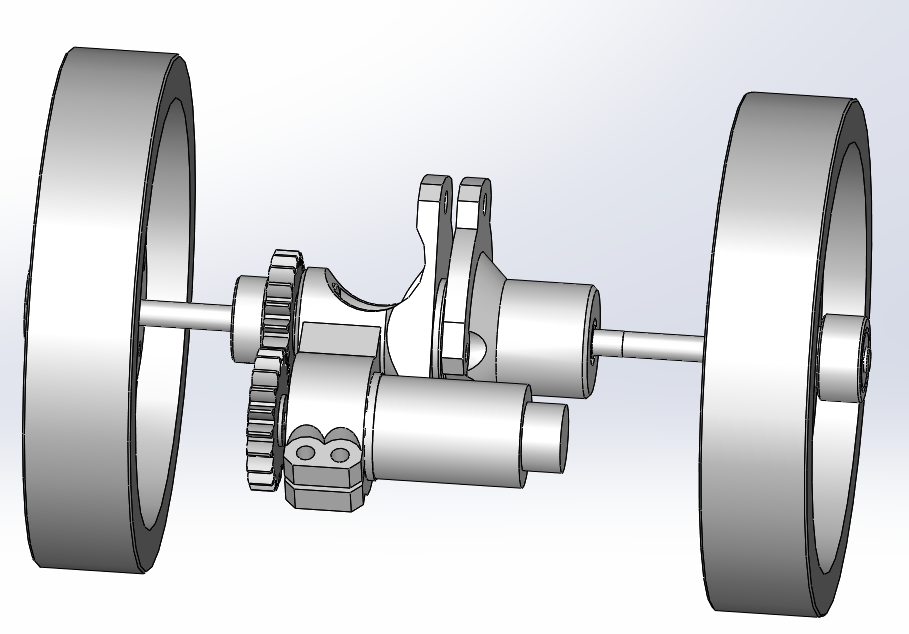
\includegraphics[width=0.5\linewidth]{BigRotorsBPR.png}%
	\caption{3Д-модель конструкции для передачи вращения от двигателя к паре больших роторов}
	\label{BigRotorsBPR}
\end{figure}

Для передачи вращения от двигателей к малым роторам используются промежуточные оси и шестерни на 12 и 20 зубьев (см. рисунок~\ref{KinemBPR}). Передаточное отношение между двигателем и каждым малым ротором составляет 1.6:1. 3Д-модель конструкции для передачи вращения от двигателя к одной паре малых роторов представлена на рисунке~\ref{SmallRotorsBPR}. Для второй пары малых роторов конструкция передачи вращения аналогичная.

\begin{figure}[!ht]
	\begin{minipage}[h]{0.5\linewidth}
		\center{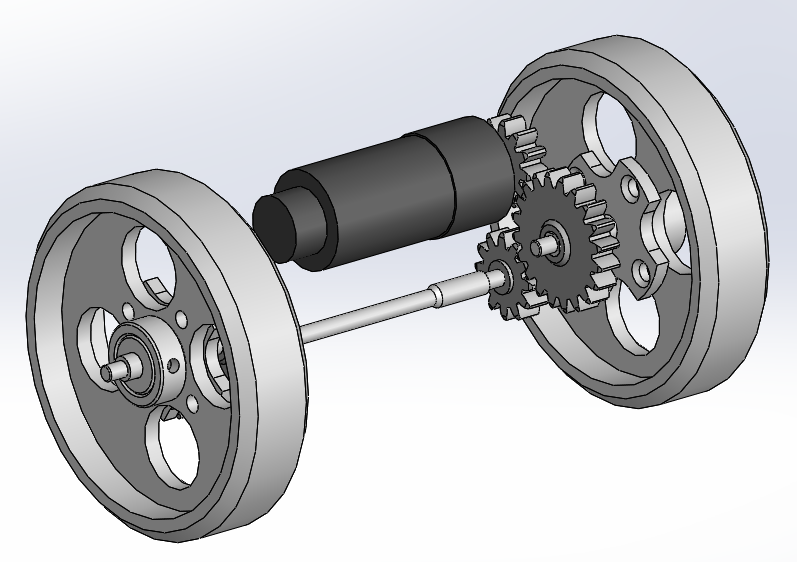
\includegraphics[width=0.8\linewidth]{SmallRotorsBPR1.png} \\ }
	\end{minipage}
	\hfill
	\begin{minipage}[h]{0.5\linewidth}
		\center{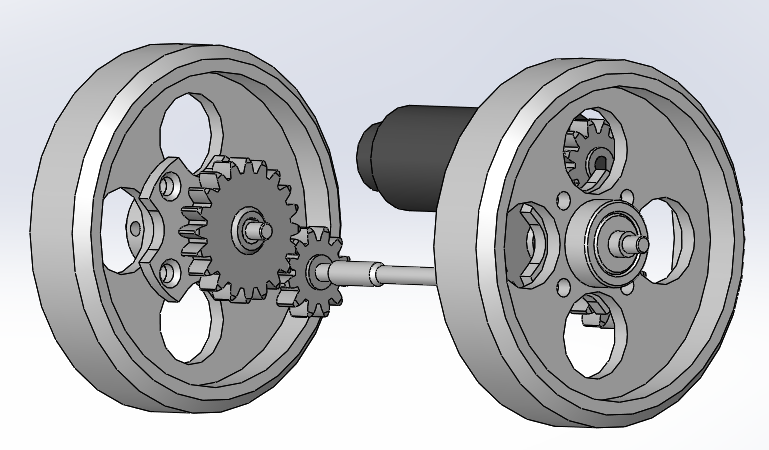
\includegraphics[width=0.9\linewidth]{SmallRotorsBPR2.png} \\ }
	\end{minipage}
	\caption{3Д-модель конструкции для передачи вращения от двигателя к паре малых роторов}
	\label{SmallRotorsBPR}
\end{figure}

На рисунке~\ref{SmallRotorsBPR3} представлено расположение двух пар малых роторов с их двигателями и элементами для передачи вращения. На рисунке~\ref{AllRotorsBPR} представлено взаимное расположение всех роторов робота.

\begin{figure}[h]
	\centering
	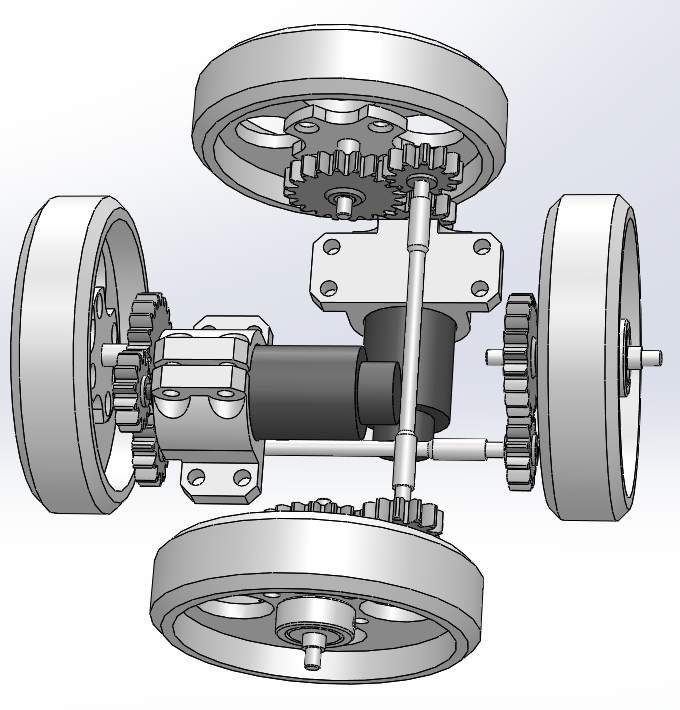
\includegraphics[width=0.5\linewidth]{SmallRotorsBPR3.png}%
	\caption{3Д-модель конструкции двух пар малых роторов с их двигателями и элементами для передачи вращения}
	\label{SmallRotorsBPR3}
\end{figure}

\begin{figure}[h]
	\centering
	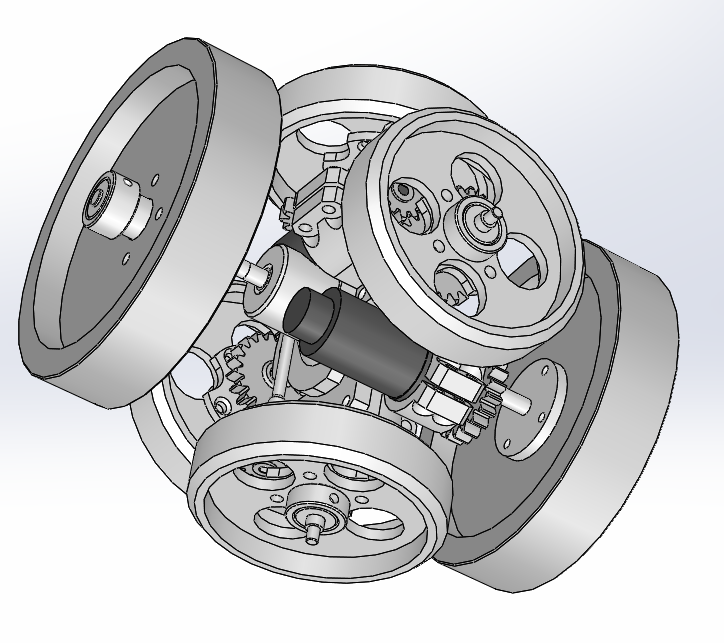
\includegraphics[width=0.5\linewidth]{AllRotorsBPR.png}%
	\caption{3Д-модель конструкции внутренних роторов безвинтового подводного робота}
	\label{AllRotorsBPR}
\end{figure}



В пространствах между большими и малыми роторами симметрично с двух сторон относительно платформы на панелях смонтированы модули питания 6, управления и связи.

В качестве модуля питания используется пара литий-полимерных (Li-Po) аккумуляторных батарей фирмы nVision (см. рисунок~\ref{Accum}) с номинальным напряжением 7.4 Вольта, емкостью 450 мАЧ и максимальным выходным током до 13.5 Ампер. Аккумуляторные батареи соединены друг с другом параллельно.

\begin{figure}[h]
	\centering
	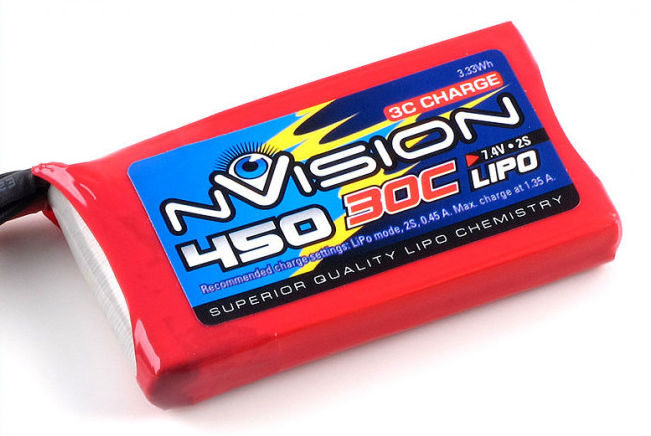
\includegraphics[width=0.5\linewidth]{Accum.png}%
	\caption{Аккумуляторная батарея фирмы nVision}
	\label{Accum}
\end{figure}

Для погружения робот оснащен механизмом регулировки плавучести. Он состоит из двух одинаковых модулей плавучести 7, размещенных и закрепленных внутри полуоболочек в наиболее удаленных частях относительно платформы. Модули плавучести имеют в своем составе лопастной насос 8 с приводом 9 на основе микроэлектродвигателя с редуктором фирмы пололу. К выходному валу электродвигателя подсоединен редуктор с передаточным отношением 75:1, далее передача вращения от редуктора к лопастному насосу осуществляется с помощью пары шестерен с передаточным отношением 1.7:1. Полости насоса --- воздушная и жидкостная имеют каналы 10, соединяющие их соответственно с внутренней полостью и внешней средой. Конструкция модуля плавучести представлена на рисунке~\ref{FloatModule}.

\begin{figure}[h]
	\centering
	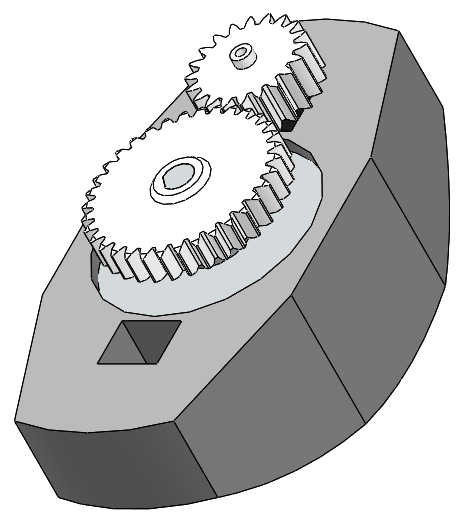
\includegraphics[width=0.4\linewidth]{FloatModule.png}%
	\caption{Конструкция модуля плавучести}
	\label{FloatModule}
\end{figure}




\section{Описание системы управления безвинтового подводного робота с внутренними роторами}

Структурная схема системы управления безвинтового подводного робота с внутренними роторами, представлена на рисунке \ref{str_scheme}.

\begin{figure}[h!]
	\begin{center}
		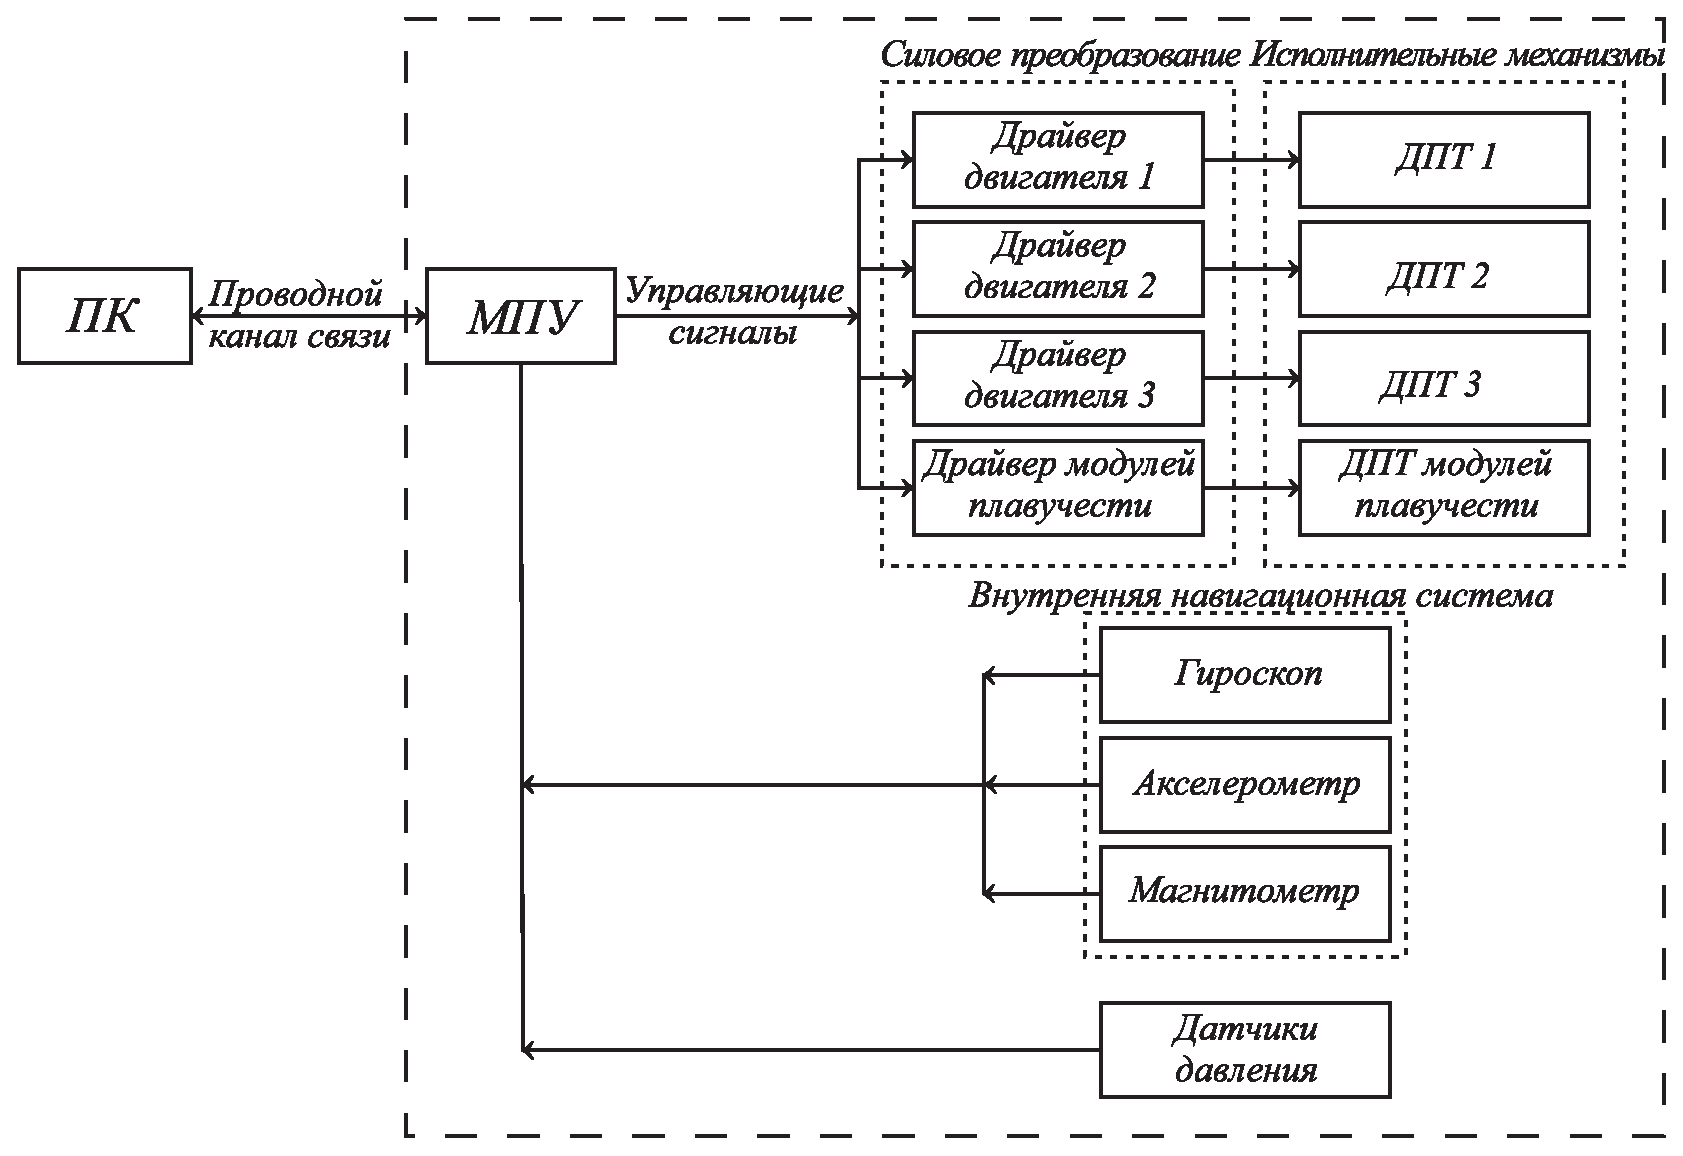
\includegraphics[width=0.8\linewidth]{StrSchemeBPR.eps}
		\caption{Структурная схема системы управления подводным роботом} \label{str_scheme}
	\end{center}
\end{figure}


\textbf{Описание микропроцессорного устройства (МПУ).} Центральным элементом системы управления является микроконтроллер LPC1768FBD100 фирмы NXP. Данный микроконтроллер имеет ядро ARM Cortex-M3, работает на частоте до 100 МГц и содержит большой набор различной периферии: 70 портов ввода-вывода; 4 таймера общего назначения с 6 выводами, имеющими возможность аппаратно формировать ШИМ-сигнал; контроллер прямого доступа в память, множество интерфейсов передачи данных. Характеристики микроконтроллера представлены в таблице~\ref{tabLpc}. В данной работе используется отладочная плата mbed NXP LPC1768 на основе вышеописанного микроконтроллера LPC1768FBD100 (см. рисунок~\ref{MbedLpc}).  Отладочная плата имеет 40-контактный DIP-форм-фактор; имеет всю необходимую обвязку элементов, необходимых для стабильной работы микроконтроллера; имеет DC-DC преобразователь, что позволяет питать плату напряжением в диапазоне от 5 до 15 вольт; позволяет загружать прошивку в микроконтроллер через USB интерфейс.

\begin{figure}[h]
	\centering
	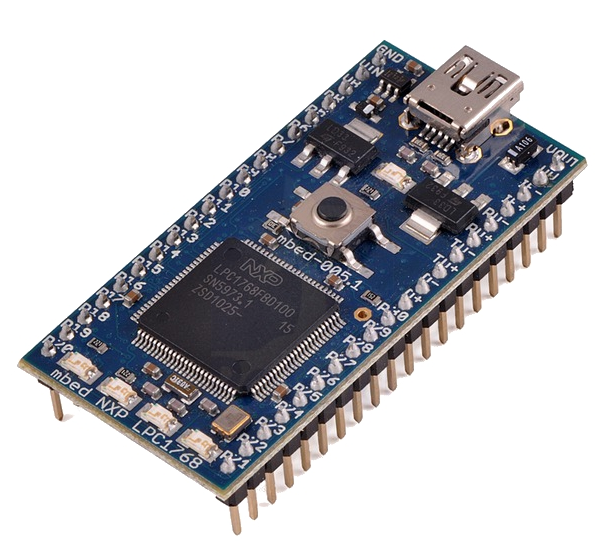
\includegraphics[width=0.4\linewidth]{MbedLpc.png}%
	\caption{Отладочная плата mbed NXP LPC1768}
	\label{MbedLpc}
\end{figure}

\begin{table}[h]
	\centering
	\caption{Характеристики микроконтроллера LPC1768FBD100}\label{tabLpc}
	\begin{tabular}{|l|c|}
		\hline
		Производитель &	NXP \\ \hline
		Корпус 	& LQFP100 \\ \hline
		Кол-во выводов 	& 100\\ \hline
		Архитектура ядра & Cortex-M3	\\ \hline
		Разрядность	& 32 бита\\ \hline
		Тактовая частота	& 100 МГц 	\\ \hline
		Оперативная память 	& 32 КБайт\\ \hline		
		Flash память & 512 КБайт\\ \hline		
		Количество входов / выходов & 70	\\ \hline
		Интерфейсы 	& Ethernet, USB, CAN, I2C, SPI, USART, I2S\\ \hline
		Разрешение АЦП & 12 бит\\ \hline
		Диапазон напряжений питания 	& 2.4...3.6 Вольт\\ \hline	
		Максимальная рабочая температура	&	$85^\circ$C 	\\ \hline
		Минимальная рабочая температура 	&	$-40^\circ$C \\ \hline	
	\end{tabular}
\end{table}

\textbf{Программа управления верхнего уровня.} Для управления безвинтовым подводным роботом с внутренними роторами на персональном компьютере разработано специальное программное обеспечение на языке C\#, окно которого представлено на рисунке~\ref{SoftHighLevel}. 

\begin{figure}[h]
	\centering
	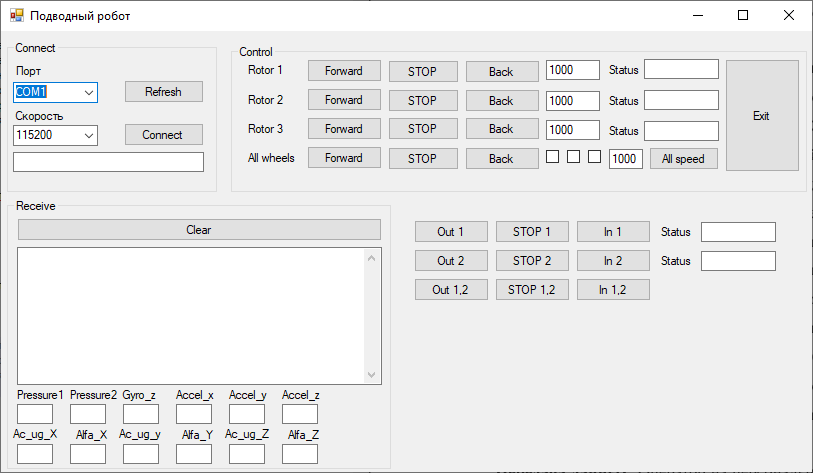
\includegraphics[width=1\linewidth]{SoftHighLevel.png}%
	\caption{Программа верхнего уровня для управления безвинтовым подводным роботом с внутренними роторами}
	\label{SoftHighLevel}
\end{figure}

В программе в группе элементов "Connect" реализованы функции выбора и подключения к необходимому СОМ-порту. В группе элементов "Control" реализованы функции управления двигателями роторов. Ниже расположены кнопки управления модулями плавучести. В группе элементов "Receive" расположено текстовое поле, в котором отображаются данные принимаемые с микроконтроллера робота, а так же маленькие текстовые поля для отображения отладочной информации: данные с датчиков давления, данные с гироскопа и акселерометра, углы ориентации робота.



\textbf{Передача данных.} Оператор на персональном компьютере (ПК, см. рисунок \ref{str_scheme}) задает команды управления подводным роботом. Команды передаются на микропроцессорное устройство (МПУ) по проводному или беспроводному (если робот находится на поверхности воды) каналу связи. Команды для двигателей представляют собой закодированные скорости вращения роторов или двигателей модулей плавучести. Протокол команд управления двигателями в общем виде представлен в таблице~\ref{tabProtokol}.

\begin{table}[h]
	\centering
	\caption{Протокол команд управления двигателями в общем виде для безвинтового подводного робота с внутренними роторами}\label{tabProtokol}
	\begin{tabular}{|c|c|c|c|}
		\hline 
		Длина пакета в байтах & Номер команды & Данные & Контрольная сумма \\ 
		\hline 
		1 байт & 1 байт & 4-6 байт & 2 байта \\ 
		\hline 
	\end{tabular} 
\end{table}

Для управления двигателями роторов используется команда 1, данными для этой команды выступают 6 байт: байт направления вращения (1 -- по часовой стрелке, 2 -- против часовой стрелки) и байт скорости вращения (об/мин) для каждого двигателя. После приема данной команды на микроконтроллере расчитывается текущий вектор гиростатического момента $\bK$, в виде которого задается управление в полученных математических моделях.

Для управления двигателями модулей плавучести используется команда 2, данными для которой выступают 4 байта: байт направления вращения и байт скорости вращения для каждого модуля плавучести.

Контрольная сумма рассчитывается по алгоритму CRC-16 CCITT.

%Передача данных для управления движением и получением дополнительной информации о состоянии системы может осуществляться по проводному и беспроводному вариантам связи. 

Проводной способ связи реализован с помощью переходника USB-USART на основе микросхемы CP2102, который подключается к USB-разъему персонального компьютера и позволяет создать виртуальный COM-порт. Для связи с микроконтроллером соответствующие выводы данного переходника подключены к выводам микроконтроллера, аппаратно поддерживающим интерфейс USART. Внешний вид переходника USB-USART представлен на рисунке~\ref{uartModules}а.

Беспроводной вариант связи реализован с помощью bluetooth-модуля HC-06, который работает аналогичным образом переходнику USB-USART: с микроконтроллером модуль НС-06 взаимодействует посредством интерфейса USART, а с компьютером bluetooth-модуль соединяется, используя профиль SPP (Serial Port Profile), что также позволяет создать виртуальный СОМ-порт и работать с ним. Внешний вид bluetooth-модуля HC-06 представлен на рисунке~\ref{uartModules}б.

\begin{figure}[!ht]
	\begin{minipage}[h]{0.5\linewidth}
		\center{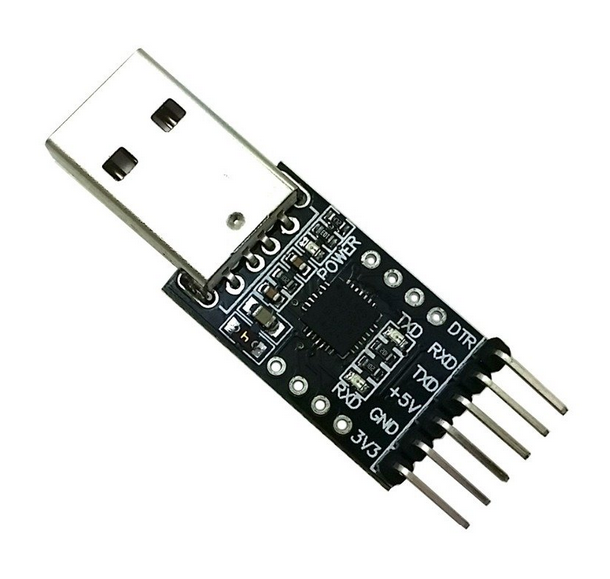
\includegraphics[height=0.7\linewidth]{Cp2102.png} }
	\end{minipage}
	\hfill
	\begin{minipage}[h]{0.5\linewidth}
		\center{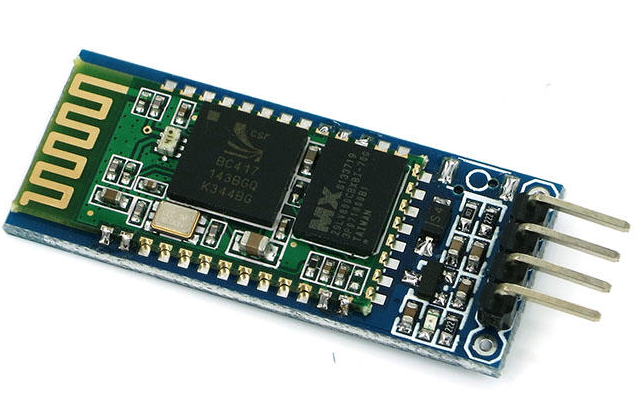
\includegraphics[height=0.6\linewidth]{HC-06.png} }
	\end{minipage}
	
	\begin{minipage}[h]{0.5\linewidth}
		\center{а}
	\end{minipage}
	\hfill
	\begin{minipage}[h]{0.5\linewidth}
		\center{б}
	\end{minipage}
	
	\caption{а) Модуль-переходник USB-USART. б) Bluetooth-модуль HC-06}
	\label{uartModules}
\end{figure}

\textbf{Управление двигателями.} Для управления отдельным двигателем роторов разработана схема, представленная на рисунке \ref{Control_system}.

\begin{figure}[h]
	\centering
	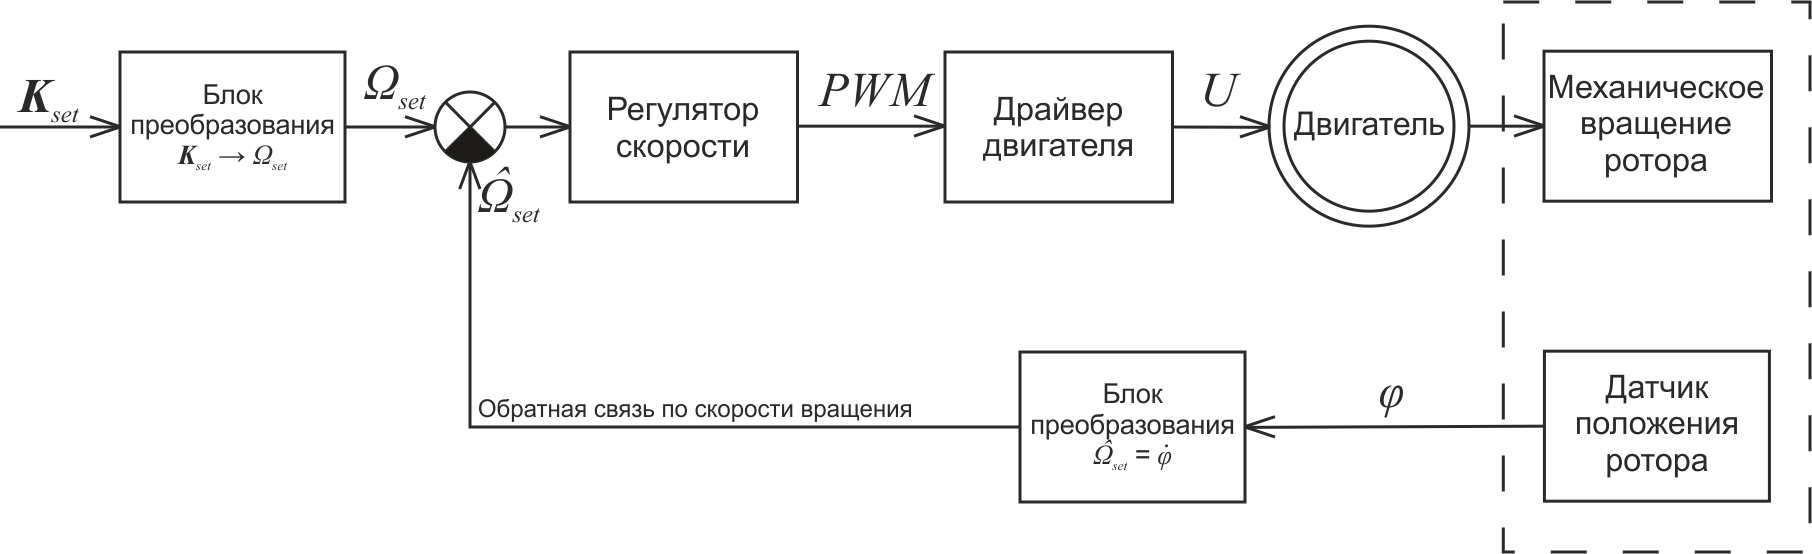
\includegraphics[width=0.9\linewidth]{Control_system.png}%
	\caption{Схема управления отдельным двигателем, где $\bK_{set}$ -- вектор внутреннего гиростатического момента; $\bOm_{set}$ -- угловая скорость вращения двигателя; $\hat{\bOm}_{set}$ -- фактическая скорость вращения двигателя; $PWM$ -- широтно-импульсная модуляция, рассчитанная для заданной скорости вращения; $U$ -- напряжение, подаваемое на двигатель; $\varphi$ -- фактическое положение ротора}
	\label{Control_system}
\end{figure}


Микропроцессор обрабатывает полученные данные и формирует управляющий сигнал, подаваемый на регулятор скорости, который представляет собой ПИ-регулятор. На выходе ПИ-регулятора получаем значение скважности ШИМ-сигнала, который формируется на выводе микроконтроллера и подается на драйвер двигателя. Драйвер двигателя усиливает сигнал с микроконтроллера, учитывая сигнал, определяющий направление вращения, и подает напряжение нужной формы непосредственно на двигатель постоянного тока.

Энкодер, расположенный на валу двигателя, фиксирует вращение вала двигателя и формирует сигнальные импульсы. Данный энкодер является инкрементальным, имеет два канала со смещением сигнала в четверть периода друг относительно друга, что позволяет определять направление вращения вала двигателя. Каждый канал формирует 12 импульсов на один оборот вала двигателя. Таким образом, используя два канала, считая переходы сигнала от низкого уровня к высокому и от высокого к низкому, можно получить 48 импульсов на один оборот вала двигателя и вычислить текущий угол поворота вала двигателя с точностью 7.5$ ^\circ$. Сигналы энкодера обрабатываются выводами микроконтроллера, настроенными на внешние прерывания.

Далее, получая изменение угла поворота вала двигателя во времени, можно рассчитать угловую скорость ротора, учитывая передаточные отношения передач между двигателем и ротором. Полученное значение является фактическим значением угловой скорости ротора и используется регулятором скорости в качестве обратной связи.

Для управления двигателями роторов используются драйверы двигателя постоянного тока VNH3SP30 фирмы STMicroelectronics. Данный драйвер обеспечивает выходной ток до 30 Ампер при напряжении от 5.5 до 36 Вольт. Драйвер содержит полномостовую схему силовых MOSFET-транзисторов, работающих в ключевом режиме, что позволяет управлять скоростью вращения и направлением вращения двигателя постоянного тока. Для данного драйвера была разработанна печатная плата, которая позволяет использовать микросхему драйвера и ее обвязку как отдельный модуль. Фото данного модуля представлено на рисунке~\ref{DriverPcb}. Характеристики данного драйвера представлены в таблице~\ref{tabVnh}

\begin{figure}[h]
	\begin{minipage}[h]{0.5\linewidth}
		\center{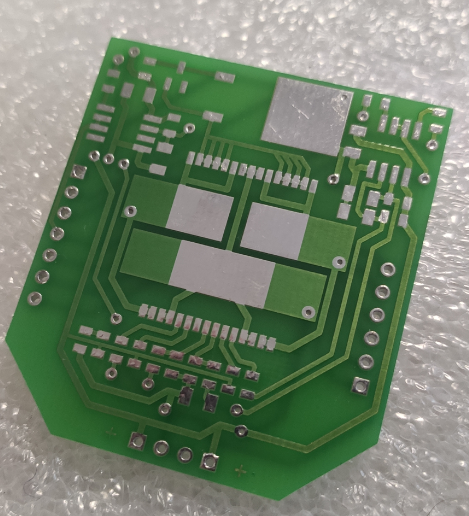
\includegraphics[height=0.8\linewidth]{DriverPcb2.png} }
	\end{minipage}
	\hfill
	\begin{minipage}[h]{0.5\linewidth}
		\center{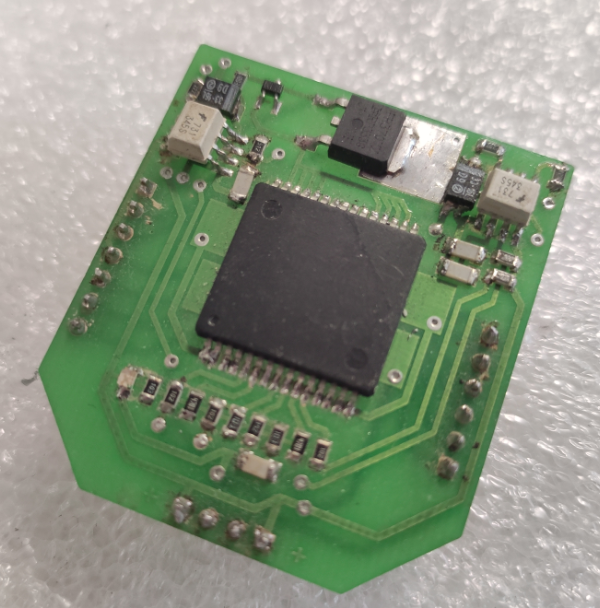
\includegraphics[height=0.8\linewidth]{DriverPcb.png} }
	\end{minipage}
	\vspace{2mm}
	\caption{Модуль управления двигателем постоянного тока на базе драйвера VNH3SP30}
	\label{DriverPcb}
\end{figure}

\begin{table}[h]
	\centering
	\caption{Характеристики драйвера двигателей постоянного тока VNH3SP30}\label{tabVnh}
	\begin{tabular}{|l|c|}
		\hline
		Количество каналов	&	1 	\\ \hline
		Максимальный пиковый ток нагрузки	&	45 А 	\\ \hline
		Максимальный непрерывный ток нагрузки  	&	30 А \\ \hline
		Максимальная частота ШИМ-сигнала 	& 10 кГц \\ \hline
		Напряжение низкого уровня управляющих сигналов &  0...1.5 В\\ \hline
		Напряжение высокого уровня управляющих сигналов &  3.25...36 В\\ \hline
		Напряжение нагрузки & 5.5...36 В \\ \hline
	\end{tabular}
\end{table}

Для управления двигателями модулей плавучести использовался драйвер двигателей постоянного тока на базе микросхемы TB6612FNG фирмы Toshiba (см. рисунок~\ref{DriverMini}), которая имеет внутри две полномостовые схемы MOSFET-транзисторов. С помощью одной микросхемы можно управлять двумя двигателями модулей плавучести. Характеристики данного драйвера представлены в таблице~\ref{tabDriverMini}.

\begin{figure}[h]
	\centering
	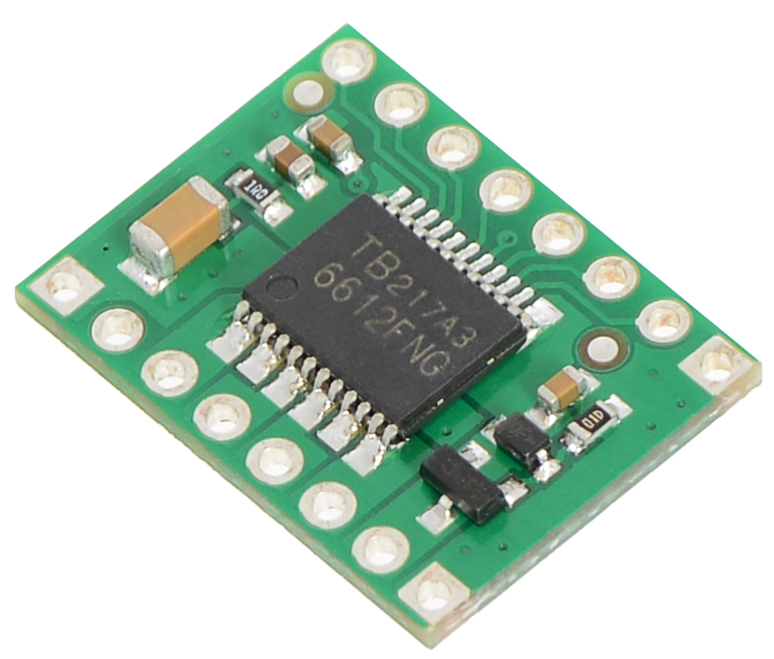
\includegraphics[width=0.4\linewidth]{DriverMini.png}%
	\caption{Драйвер двигателей постоянного тока на базе микросхемы TB6612FNG}
	\label{DriverMini}
\end{figure}

\begin{table}[h]
	\centering
	\caption{Характеристики драйвера двигателей постоянного тока TB6612FNG}\label{tabDriverMini}
	\begin{tabular}{|l|c|}
		\hline
		Количество каналов	&	2 	\\ \hline
		Максимальный пиковый ток нагрузки на канал	&	3 А 	\\ \hline
		Максимальный непрерывный ток нагрузки на канал 	&	1 А \\ \hline
		Максимальная частота ШИМ-сигнала 	& 100 кГц \\ \hline
		Напряжение управляющих сигналов &  2.7...5.5 В\\ \hline
		Напряжение нагрузки & 4.5...13.5 В \\ \hline
	\end{tabular}
\end{table}


\textbf{Описание датчиков.} Для определения ориентации робот имеет датчик на основе микросхемы MPU9250 (см. рисунок~\ref{Mpu9250}), который включает в себя трехосевой акселерометр, трехосевой гироскоп и трехосевой магнитометр. Данный датчик является цифровым, имеет на борту 16-битный аналого-цифровой преобразователь для оцифровки аналоговых данных с каждого сенсора. Датчик может быть подключен к микроконтроллеру по интерфейсам SPI или I2C. Характеристики датчика представлены в таблице~\ref{tabMpu}.

\begin{figure}[h]
	\centering
	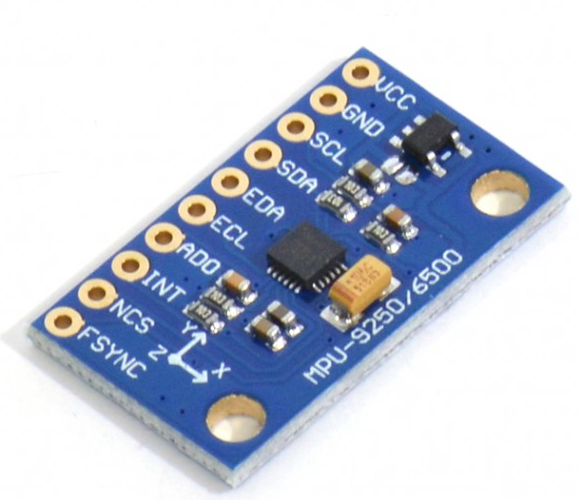
\includegraphics[width=0.3\linewidth]{Mpu9250.png}%
	\caption{Датчик MPU9250}
	\label{Mpu9250}
\end{figure}

\begin{table}[h]
	\centering
	\caption{Характеристики датчика MPU9250}\label{tabMpu}
	\begin{tabular}{|l|c|}
		\hline
		Рабочие диапазоны гироскопа & ±250, ±500, ±1000, ±2000 $^\circ$/с \\ \hline
		Чувствительность гироскопа & 131, 65.5, 32.8, 16.4 LSB/$^\circ$/c \\ \hline
		Рабочие диапазоны акселерометра & ±2, ±4, ±8, ±16 g\\ \hline
		Рабочий диапазон магнитометра & ±4800 мкТл\\ \hline
		Напряжение питания & 2.4...3.6 В\\ \hline
		Рабочий ток гироскопа & 3.2 мА\\ \hline
		Рабочий ток акселерометра & 450 мкА\\ \hline
		Рабочий ток магнитометра & 280 мкА\\ \hline
		Ток в режиме сна & 16 мкА \\ \hline
		Максимальная рабочая температура	&	$125^\circ$C 	\\ \hline
		Минимальная рабочая температура 	&	$-40^\circ$C \\ \hline
	\end{tabular}
\end{table}

Для расчёта ориентации объекта в пространстве по показаниям датчиков акселерометра, гироскопа и магнитометра использовался фильтр Маджвика (Madgwick filter)~\cite{Madgwick}. Данный фильтр имеет две разновидности: IMU -- берет в  расчет данные с акселерометра и гироскопа, MARG -- учитывает данные с гироскопа, акселерометра и магнитометра. В данной работе использовался фильтр MARG, который, по сравнению с фильтром IMU, учитывает магнитные искажения и компенсирует смещения гироскопа. На выходе фильтра получаем кватернион, который описывает вращение объекта вокруг произвольной оси. Кватернион можно преобразовать в углы Эйлера, которые определяют углы крена, тангажа и рысканья. Точность определения углов ориентации объекта: 0.6$^\circ$ -- среднеквадратичное отклонение в неподвижном состоянии; 0.8$^\circ$ -- среднеквадратичное отклонение в подвижном состоянии.

На каждое обновление фильтра MARG необходимо выполнить 277 простых арифметических операций. Данный фильтр можно использовать с частотой обновления от 10 Гц. Из-за невысокой вычислительной нагрузки и возможности работать на низких частотах дискретизации данный фильтр подходит для вычисления углов ориентации на микроконтроллере. 





Для контроля глубины робот оснащен двумя датчиками давления MPX5010GP фирмы NXP (см. рисунок~\ref{PressureSensor}), расположенными рядом с модулями плавучести. Датчик является аналоговым, максимальная величина измеряемого давления -- 10 кПа, что соотвествует 1019.78 мм глубины погружения в воде. Датчик подключается к входу 12-битного аналого-цифрового преобразователя (АЦП) микроконтроллера. Характеристики датчика представлены в таблице~\ref{tabPressure}.

\begin{figure}[h]
	\centering
	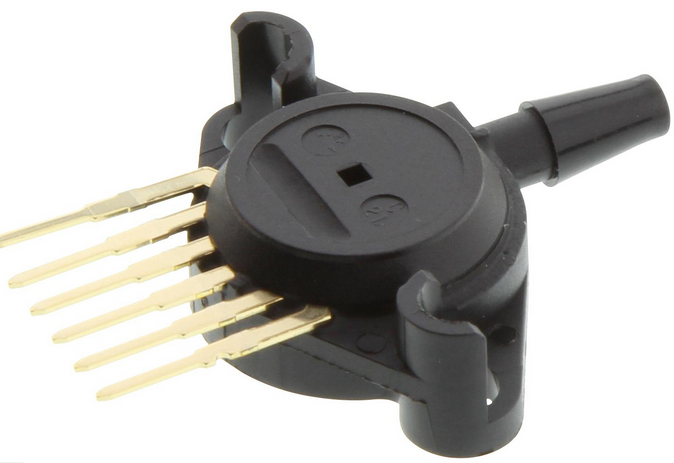
\includegraphics[width=0.5\linewidth]{PressureSensor.png}%
	\caption{Датчик давления MPX5010GP фирмы NXP}
	\label{PressureSensor}
\end{figure}

\begin{table}[h]
	\centering
	\caption{Характеристики датчика давления MPX5010GP фирмы NXP}\label{tabPressure}
	\begin{tabular}{|l|c|}
		\hline
		Максимальное рабочее давление	&	10 кПа 	\\ \hline
		Предельно допустимое давление & 40 кПа \\ \hline
		Чувствительность в жидкости	& 4.413 мВ/мм \\ \hline
		Время отклика 	& 1 мс \\ \hline
		Выходное напряжение при максимальном давлении	&  4.7 В\\ \hline
		Напряжение питания 	& 5 В\\ \hline	
		Потребляемый ток	& 5...10 мА\\ \hline	
		Точность	& 5\% \\ \hline
		Максимальная рабочая температура	&	$125^\circ$ C 	\\ \hline
		Минимальная рабочая температура 	&	$-40^\circ$ C \\ \hline
	\end{tabular}
\end{table}

Рассчитаем минимальное изменение глубины, которое может воспринимать датчик давления. Так как опорное напряжение АЦП микроконтроллера -- 3.3 Вольта, для преобразования выходного сигнала датчика, имеющего максимальное значение в 4.7 вольта, использовался делитель напряжения на резисторах номиналами 10 кОм и 15 кОм. Коэффициент преобразования данного делителя напряжения -- 1.67, следовательно максимальное напряжение, поступающее на вход АЦП микроконтроллера, составит 2.81 В. АЦП, к которому подключены датчики давления является 12-ти разрядным с опорным напряжением 3.3 В. Поэтому разрешающая способность данного АЦП -- 3.2 мВ, а до делителя напряжения 5.12 мВ. Таким образом, можно определять изменение глубины на 1.16 мм.



\textbf{Плата управления} с электронными компонентами, разработанная для безвинтового подводного робота с внутренними роторами представлена на рисунке~\ref{PCB_BPR}

\begin{figure}[h!]
	\begin{center}
		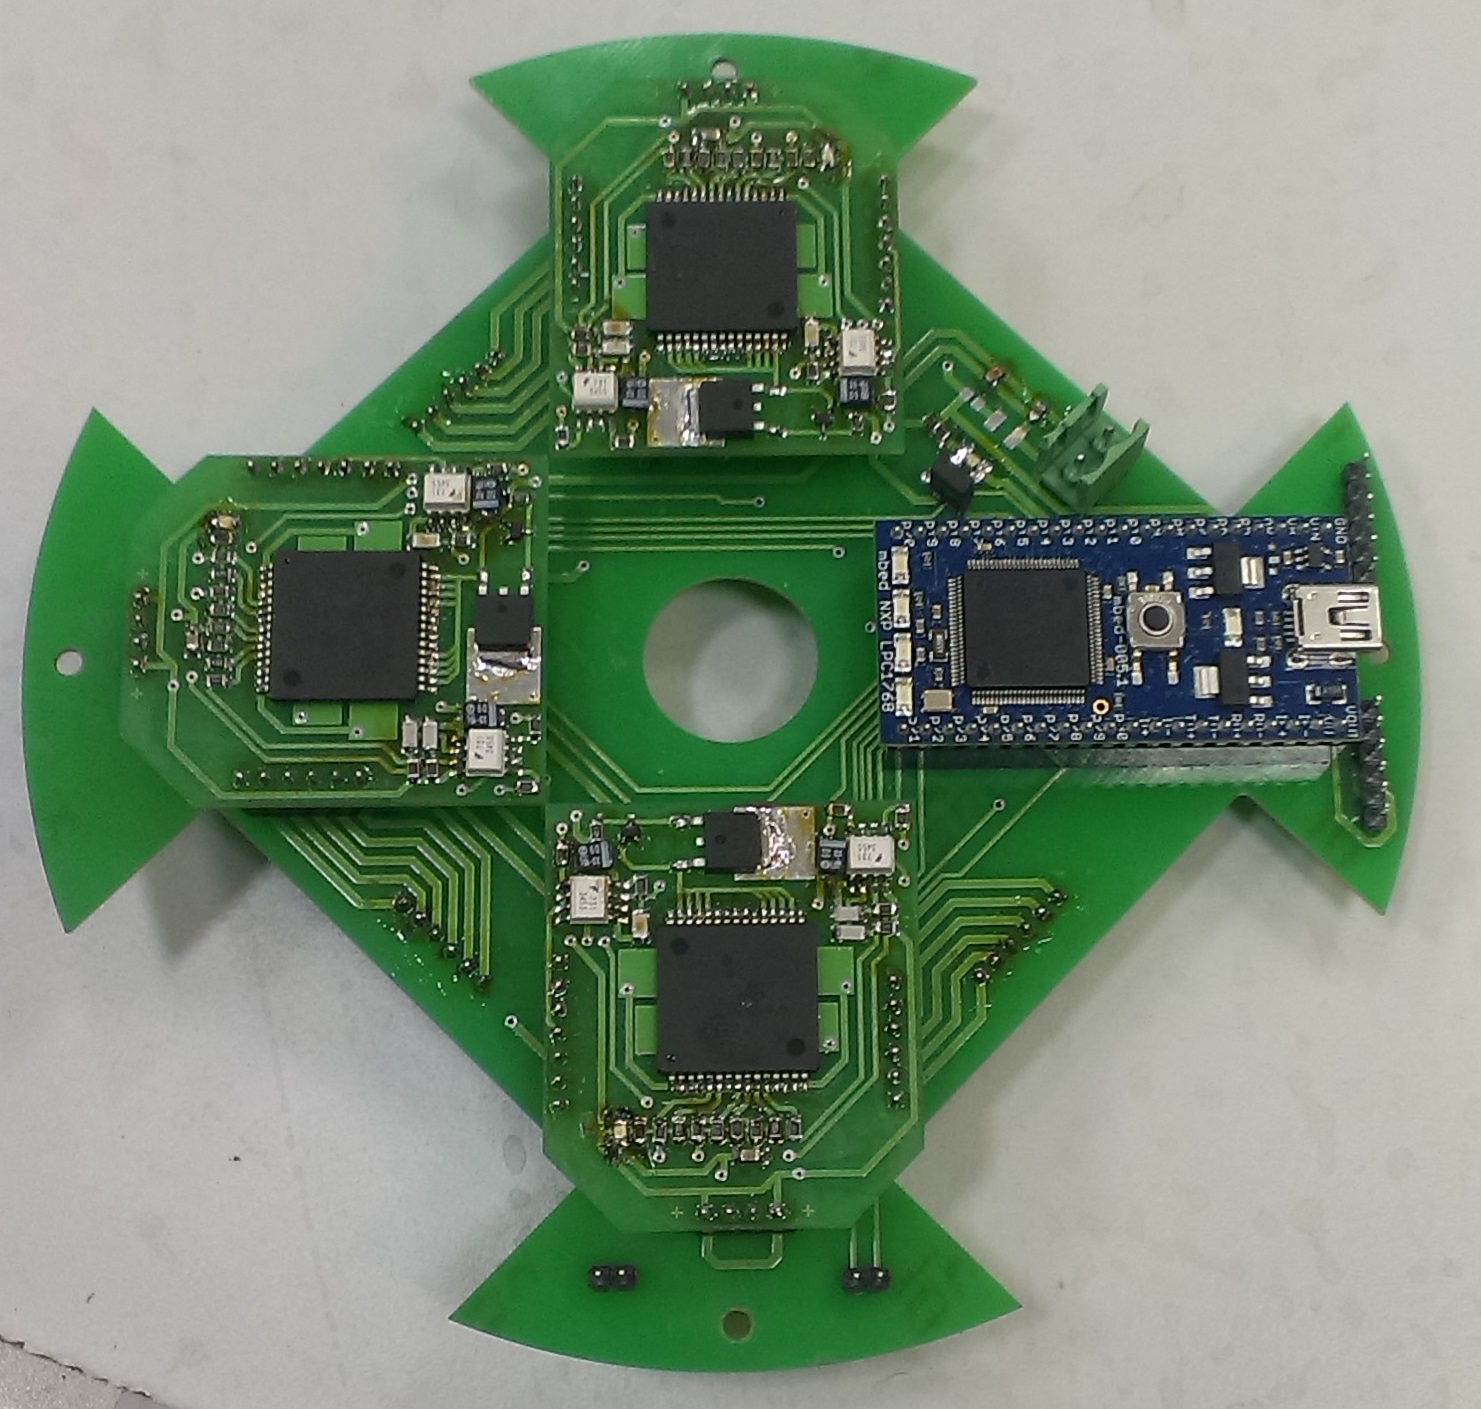
\includegraphics[width=0.8\linewidth]{PCB_BPR.png}
		\caption{Плата управления безвинтового подводного робота с внутренними роторами} \label{PCB_BPR}
	\end{center}
\end{figure}

%Управление осуществляется с персонального компьютера (ПК), для которого было разработано специальное программное обеспечение. Для управления роботом необходимо задать направления и скорости вращения каждого из роторов, а также время разгона до заданной скорости. Отдельно осуществляется управление модулями плавучести, которые отвечают за погружение робота.













\clearpage           % Глава 3
\chapter{Результаты экспериментальных исследований водоплавающего мобильного робота в форме эллипсоида}\label{ch:ch4}

\section{Методика проведения экспериментальных исследований}\label{sec:ch4/sec1}

Эксперименты проводились в бассейне размерами 3 х 1.5 x 1.5 метра, заполненным водой. При движении робота траектория отслеживалась с помощью системы захвата движения фирмы Vicon, которая состоит из 4 камер, расположенных по периметру области съемки. Камеры предназначены для работы под водой. 

Для работы с системой камер используется программное обеспечение Vicon Motus. Перед каждым экспериментом система калибруется, используя специальный калибровочный объект. Далее на отслеживаемый объект устанавливаются активные маркеры таким образом, чтобы в каждый момент времени каждый маркер был в кадре минимум двух камер. После записи и обработки видео получаем траекторию движения объекта и проекции единичных векторов, связанных с осями подвижной системы координат, расположенной на объекте на глобальную неподвижную систему координат. Данные проекции образуют матрицу поворота объекта, которая связывает неподвижную и подвижную системы координат.

\section{Проведение экспериментальных исследований}\label{subsec:ch4/sec2/sub1}

Цель экспериментов -- определение характера движения безвинтового подводного робота при различных управляющих воздействиях. В качестве управляющих воздействий выступают гиростатические моменты роторов K1, K2, K3, возникающие при их вращении. Рассмотрены три серии экспериментов: вращение только пары больших роторов, вращение только одной пары меньших роторов и одновременное вращение пары больших и одной пары меньших роторов. В каждом эксперименте роторы разгонялись до максимальной скорости 590 об/мин.

Так как роторы 2 и 3 имеют одинаковые массо-геометрические характеристики и лежат в одной плоскости, их совместное вращение приведет к качественно аналогичному, результату, что и в случае их вращения по отдельности.


1.	Вращение пары больших роторов. В качестве управляющего воздействия выступала угловая скорость пары больших роторов, ось вращения которых совпадает с большей полуосью эллипсоида. Роторы разгонялись до максимальной скорости 590 об/мин, которая поддерживалась постоянной в течение 3 секунд. Вектор внутреннего гиростатического момента, сообщенный телу после разгона роторов, $K = (2i_1\omega_{max}, 0, 0)$. Положение робота в начальный момент времени и момент времени $t=3$ секунды после начала движения, для отдельного эксперимента представлено на рисунке \ref{BPR_exp1}.

\begin{figure}[h]
	\begin{minipage}[h]{0.5\linewidth}
		\center{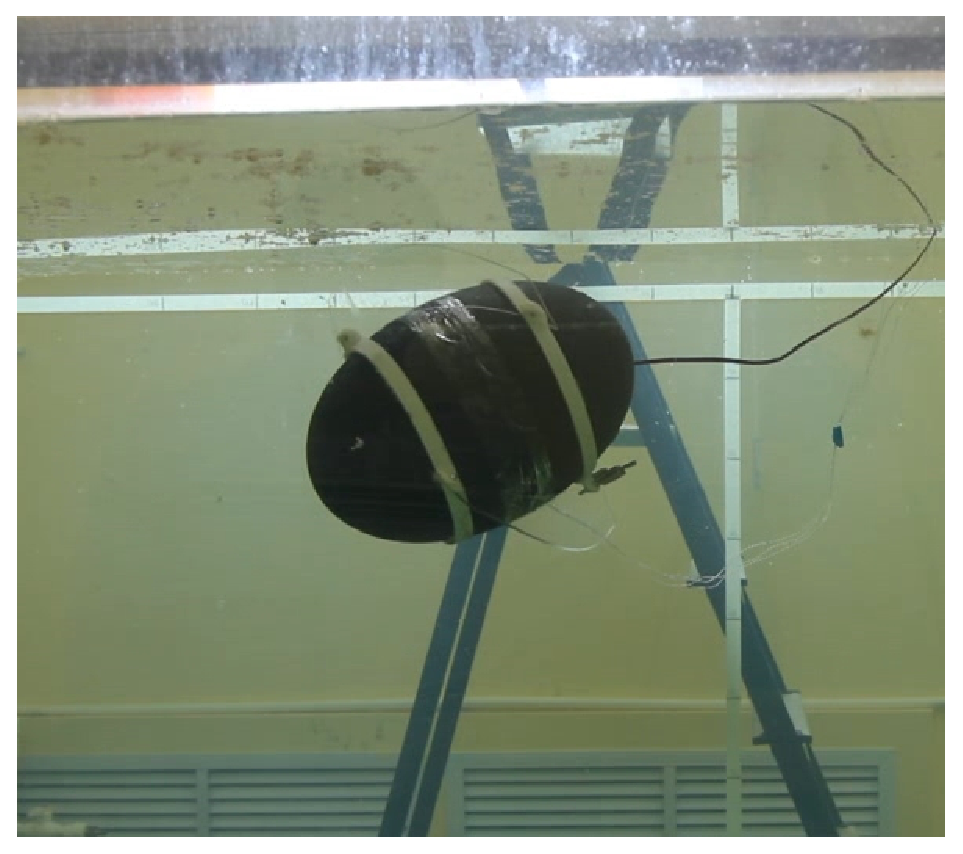
\includegraphics[width=0.7\linewidth]{exp11.eps} \\ а)}
	\end{minipage}
	\begin{minipage}[h]{0.5\linewidth}
		\center{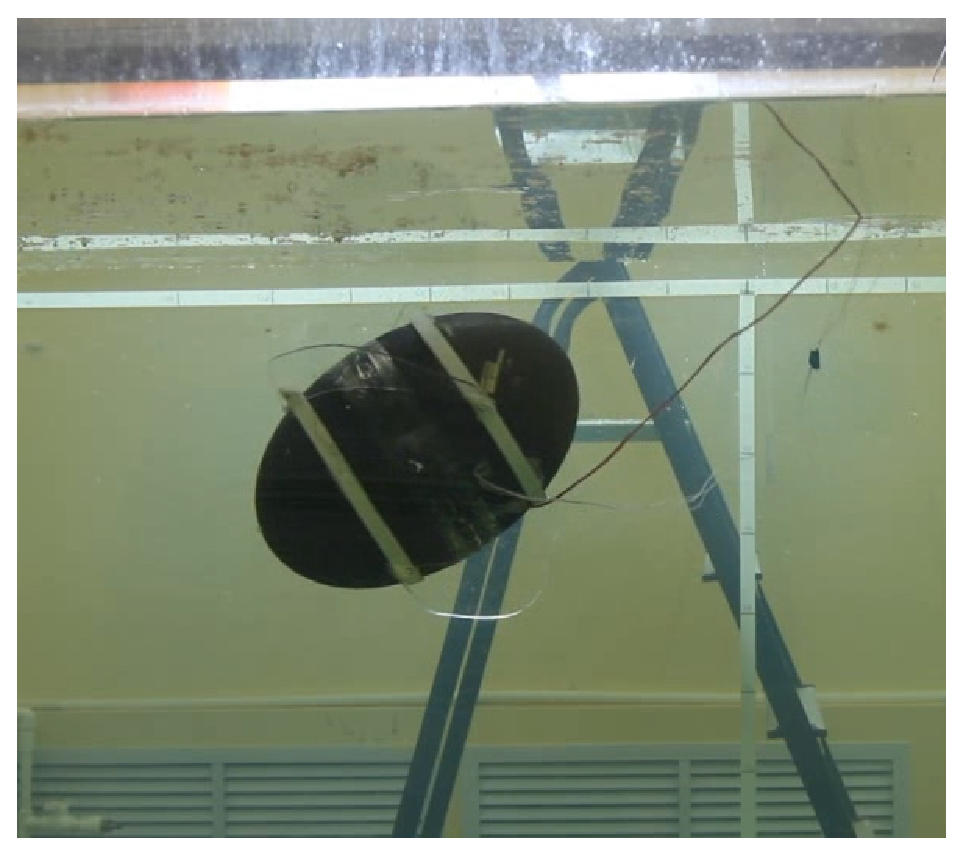
\includegraphics[width=0.7\linewidth]{exp12.eps} \\ б)}
	\end{minipage}
	\caption{Положение робота а) в начальный момент времени и б) момент времени t=3 секунды от начала движения при $\bK=(2i_1\omega_{max},  0,  0)$ }
	\label{BPR_exp1}
\end{figure}

Для данных управляющих воздействий проведена серия из трех экспериментов. Среднее изменение координат геометрического центра робота и изменение углов, определяющих положение, для трех экспериментов составили:

\begin{center}
$\Delta x_{exp}=0.115 \;\mbox{м},\; \Delta y_{exp}=0.010\; \mbox{м},\; \Delta z_{exp}=0.055\; \mbox{м};$ \\ 
$\Delta \theta_{exp}=4^{\circ},\; \Delta \psi_{exp}=10^{\circ},\; \Delta \varphi_{exp}=120^{\circ}.$
\end{center}

Здесь и далее $x_{exp},\;y_{exp},\;z_{exp}$ --- координаты геометрического центра безвинтового подводного робота, $\theta_{exp}$ --- угол дифферента --- угол между осью вращения эллипсоида и горизонтальной плоскостью; $\psi_{exp}$ --- угол курса --- угол между осью вращения эллипсоида и вертикальной плоскостью (этот угол сходен с углом курса судна, но отсчитывается в соответствии с выбранной системой координат); $\varphi_{exp}$ --- угол вращения --- угол, определяющий поворот робота вокруг оси вращения эллипсоида.

%Траектории движения полученные в результате численного моделирования при вышеописанных управляющих воздействиях и экспериментальные траектории движения робота представлены на рисунке \ref{Exp_BPR_1}.
%
%\begin{figure}[ht]
%	\centering
%	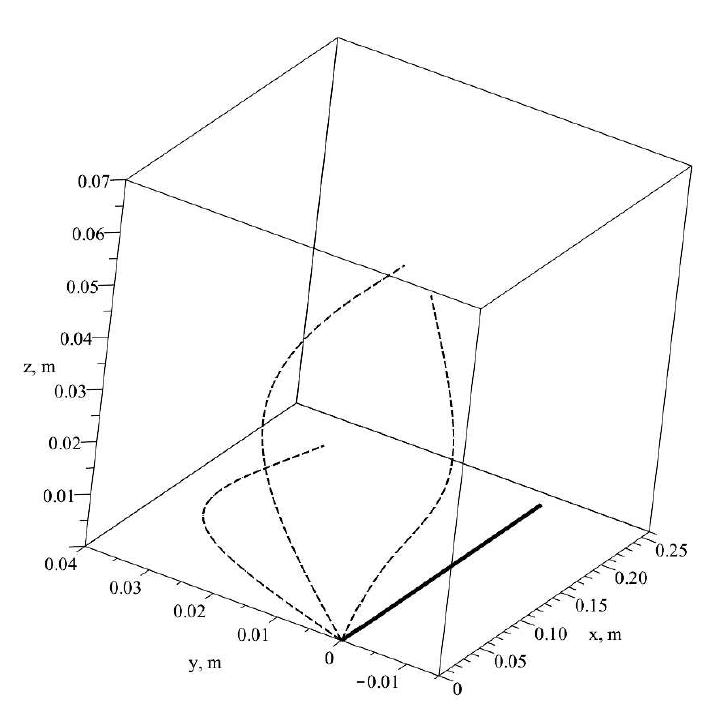
\includegraphics[width=0.5\linewidth]{Exp_BPR_1.png}%
%	\caption{Теоретическая (сплошная линия) и экспериментальные (штриховые линии) траектории движения безвинтового подводного робота при $K = (2i_1\omega_{max}, 0, 0)$}
%	\label{Exp_BPR_1}
%\end{figure}


2.	Вращение одной пары малых роторов. В качестве управляющего воздействия выступала угловая скорость одной пары малых роторов. Роторы разгонялись до максимальной скорости 590 об/мин, которая поддерживалась постоянной в течение 3 секунд. Вектор гиростатического момента, сообщенный телу после разгона роторов, $K = (0, 2i_2\omega_{max}, 0)$. Положение робота в начальный момент времени и момент времени $t=3$ секунды после начала движения, для отдельного эксперимента представлено на рисунке \ref{BPR_exp2}.

% Разгон маховика до данной скорости выполняется за время $t_{acc}=0.7$ с.

\begin{figure}[h]
	\begin{minipage}[h]{0.5\linewidth}
		\center{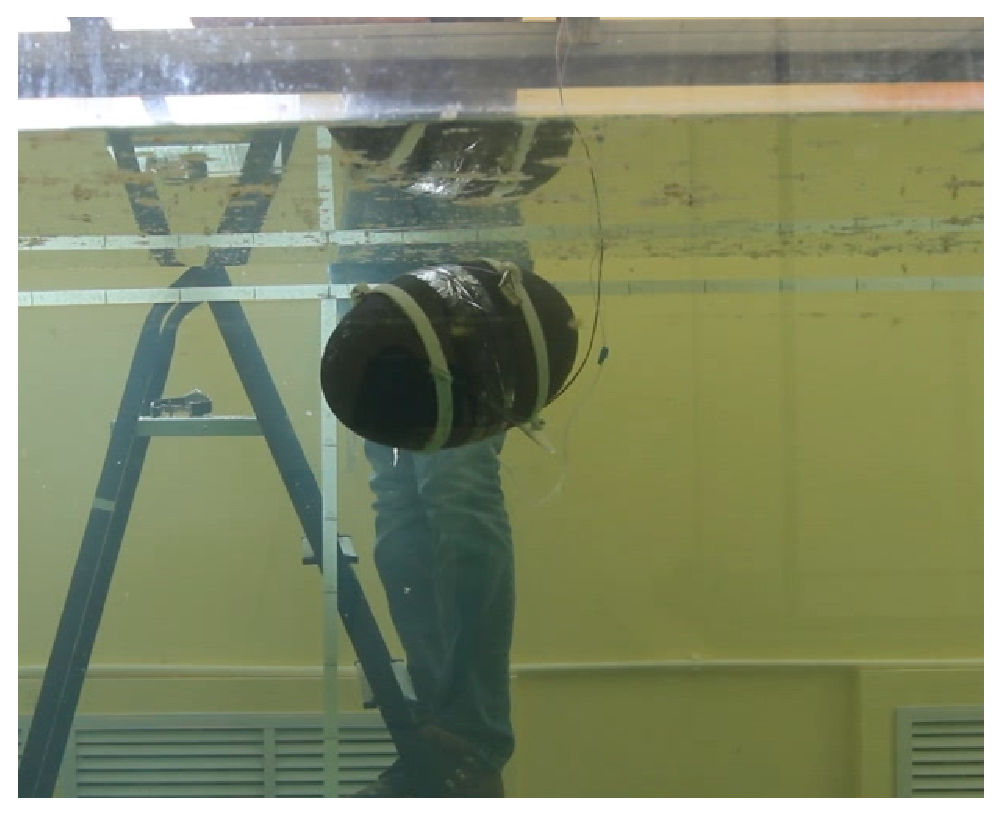
\includegraphics[width=0.7\linewidth]{exp21.eps} \\ а)}
	\end{minipage}
	\begin{minipage}[h]{0.5\linewidth}
		\center{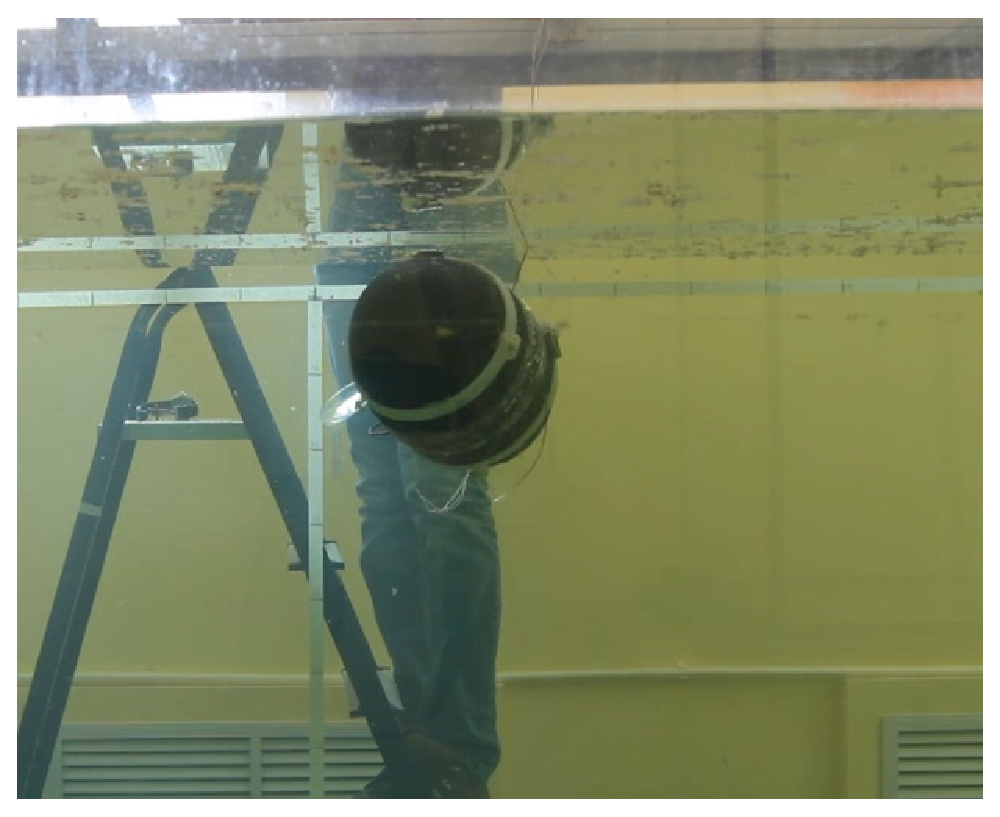
\includegraphics[width=0.7\linewidth]{exp22.eps} \\ б)}
	\end{minipage}
	\caption{Положение робота а) в начальный момент времени и б) момент времени t=3 секунды от начала движения при $\bK=(0,  2i_2\omega_{max}, 0)$}
	\label{BPR_exp2}
\end{figure}

Для данных управляющих воздействий проведена серия из трех экспериментов. Среднее изменение координат геометрического центра робота и изменение углов, определяющих положение, для данной серии экспериментов составили:

\begin{center}
$\Delta x_{exp}=0.054\; \mbox{м},\; \Delta y_{exp}=0.008\,\; \mbox{м},\; \Delta z_{exp}=0.068\; \mbox{м},\;$ \\
$\Delta \theta_{exp}=61^{\circ},\; \Delta \psi_{exp}=62^{\circ},\; \Delta \varphi_{exp}=10^{\circ}.$
\end{center}

%Траектории движения полученные в результате численного моделирования при вышеописанных управляющих воздействиях и экспериментальные траектории движения робота представлены на рисунке \ref{Exp_BPR_2}.
%
%\begin{figure}[ht]
%	\centering
%	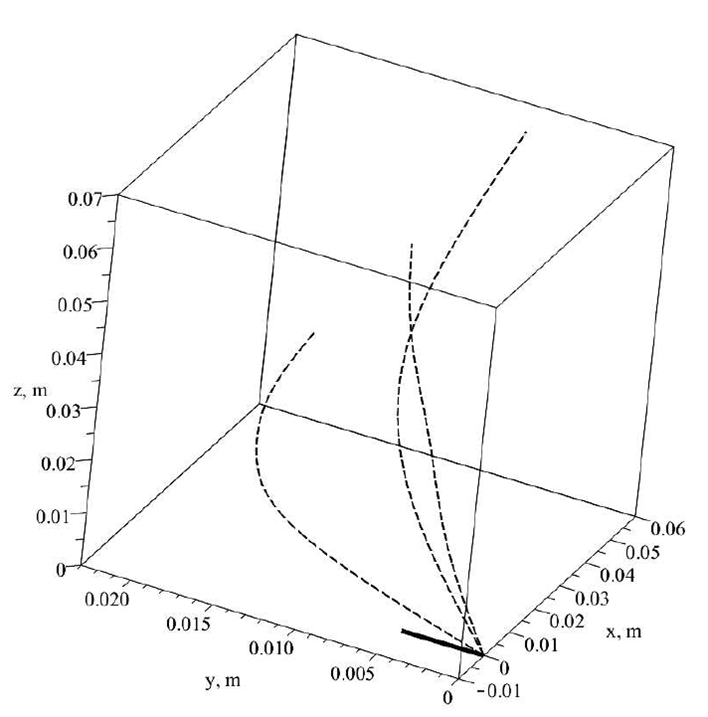
\includegraphics[width=0.5\linewidth]{Exp_BPR_2.png}%
%	\caption{Теоретическая (сплошная линия) и экспериментальные (штриховые линии) траектории движения безвинтового подводного робота при $K = (0, 2i_2\omega_{max}, 0)$}
%	\label{Exp_BPR_2}
%\end{figure}


3.	Вращение пары больших роторов и одной пары малых роторов. В качестве управляющего воздействия выступала угловая скорость одной пары малых и пары больших роторов. Роторы разгонялись до максимальной скорости 590 об/мин, которая поддерживалась постоянной в течение 3 секунд. Вектор гиростатического момента, сообщенный телу после разгона роторов, $K = (2i_1\omega_{max}, 2i_2\omega_{max}, 0)$. Положение робота в начальный момент времени и момент времени $t=3$ секунды после начала движения, для отдельного эксперимента представлено на рисунке \ref{BPR_exp3}.

\begin{figure}[h]
	\begin{minipage}[h]{0.5\linewidth}
		\center{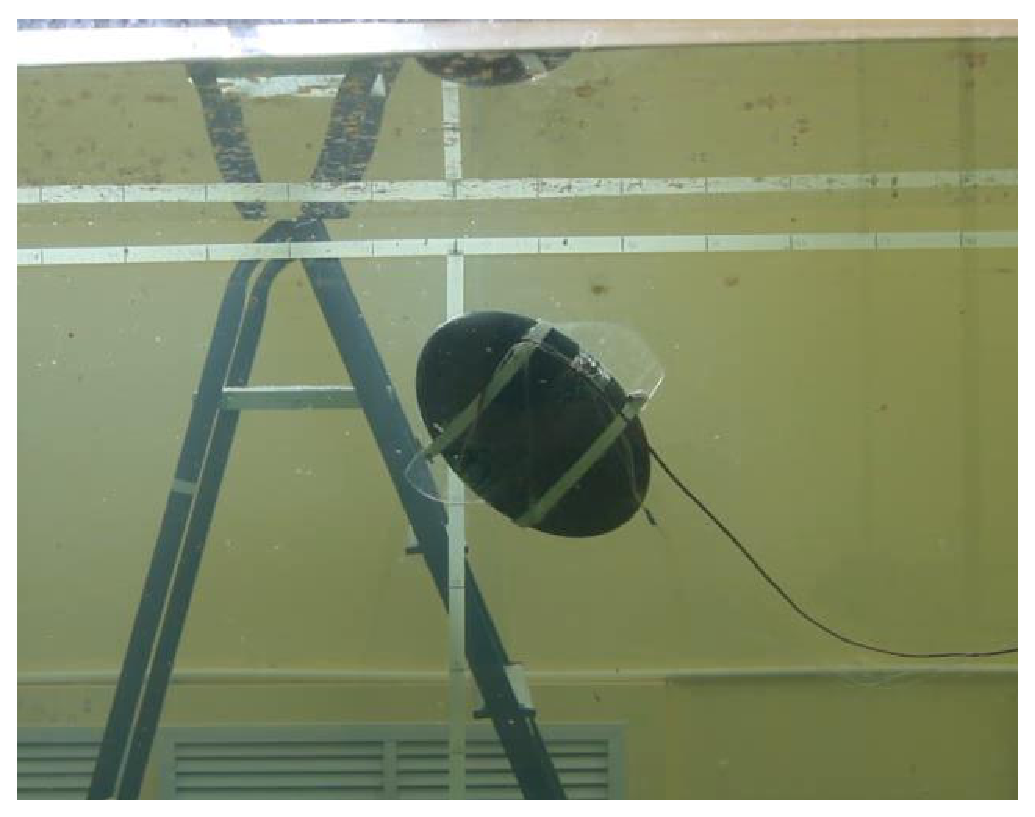
\includegraphics[width=0.7\linewidth]{exp31.eps} \\ а)}
	\end{minipage}
	\begin{minipage}[h]{0.5\linewidth}
		\center{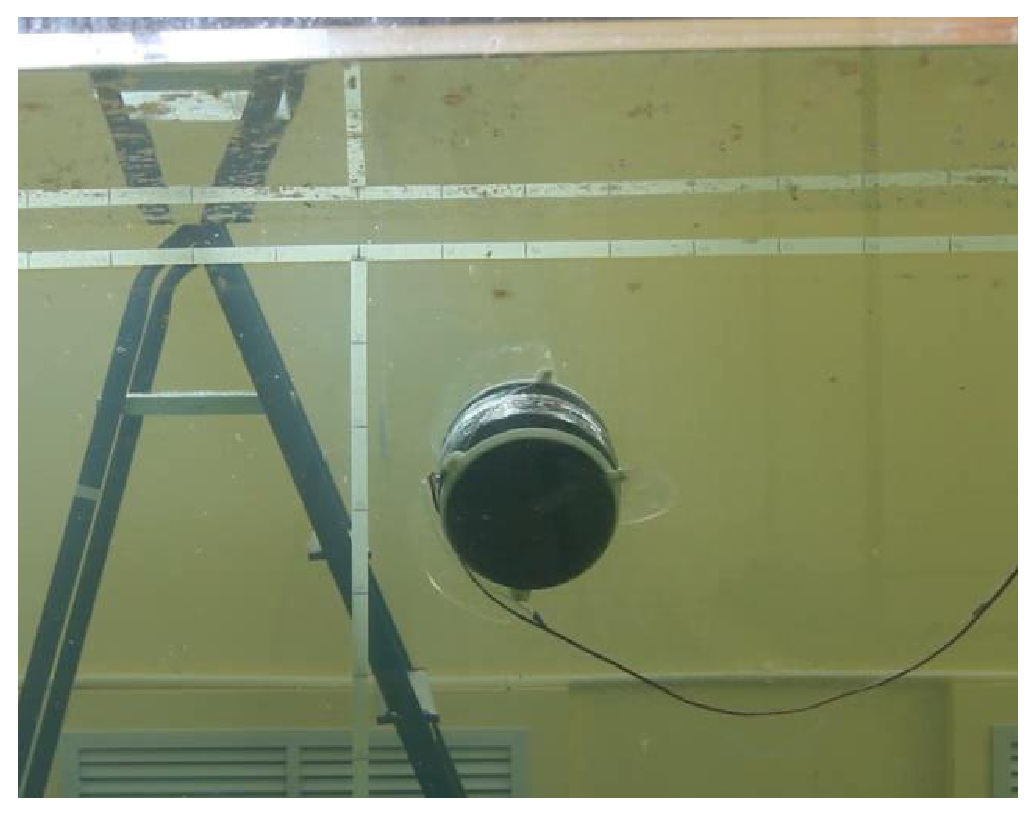
\includegraphics[width=0.7\linewidth]{exp32.eps} \\ б)}
	\end{minipage}
	\caption{Положение робота а) в начальный момент времени и б) момент времени t=3 секунды от начала движения при $\bK=(2i_1\omega_{max}, 2i_2\omega_{max}, 0)$}
	\label{BPR_exp3}
\end{figure}

Для данных управляющих воздействий проведена серия из трех экспериментов. Среднее изменение координат геометрического центра робота и изменение углов, определяющих положение, для данной серии экспериментов составили:

\begin{center}
$\Delta x_{exp}=0.106\; \mbox{м}, \; \Delta y_{exp}=0.050\; \mbox{м},\; \Delta z_{exp}=0.053\; \mbox{м}, \;$ \\
%\item $|r|=0.129$ м;
$\Delta \theta_{exp}=17^{\circ},\; \Delta \psi_{exp}=90^{\circ},\; \Delta \varphi_{exp}=51^{\circ}.$
\end{center}

%Траектории движения полученные в результате численного моделирования при вышеописанных управляющих воздействиях и экспериментальные траектории движения робота представлены на рисунке \ref{Exp_BPR_3}.
%
%\begin{figure}[ht]
%	\centering
%	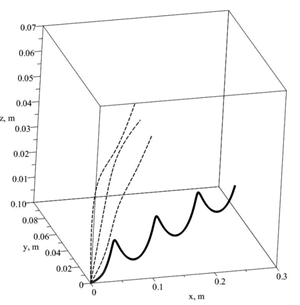
\includegraphics[width=0.5\linewidth]{Exp_BPR_3.png}%
%	\caption{Теоретическая (сплошная линия) и экспериментальные (штриховые линии) траектории движения безвинтового подводного робота при $K = (2i_1\omega_{max}, 2i_2\omega_{max}, 0)$}
%	\label{Exp_BPR_3}
%\end{figure}

Проведенные эксперименты подтвердили возможность реализации движения в жидкости за счет изменения внутреннего гиростатического момента.

%Несмотря на указанную теоретическую возможность перемещения подводного робота с помощью вращения роторов, экспериментальные данные существенно отличаются от результатов, полученных в рамках модели идеальной жидкости. Например, при первых двух вариантах управляющих воздействий в рамках теоретической модели робот движется прямолинейно не изменяя своей ориентации. При проведении экспериментов такого движения добиться не удается. Кроме того, перемещение безвинтового подводного робота на практике в два раза меньше теоретического.

\section{Оценка экспериментальных данных}\label{subsec:ch4/sec2/sub2}

\textbf{1. Вращение пары больших роторов.} Траектория движения, полученная в результате численного моделирования при управляющих воздействиях, заданных в виде $\bK=\begin{pmatrix} 2i_1\omega_{max},  0,  0 \end{pmatrix}$, и экспериментальная траектория движения приведены на рисунке \ref{traj1}. После движения с заданными управляющими воздействиями в течение 3 секунд линейная и угловая скорость составили $\bV_t=\begin{pmatrix} 0.0916,  0, 0 \end{pmatrix}$ м/с, ${\bOm}_t=\begin{pmatrix} 41.0125, 0, 0 \end{pmatrix}$ об/мин. А изменение его ориентации  определяется углами: $\Delta \theta_t=0^{\circ},\; \Delta \psi_t=0^{\circ},\; \Delta \varphi_t=738.2^{\circ}$. При данном управляющем воздействии по результатам численного моделирования, робот проходит расстояние $|\br_t|=0.275$ м, а среднее значение перемещения по экспериментальным данным $|\br_{exp}|=0.128$ м.


\begin{figure}[h!]
	\begin{center}
		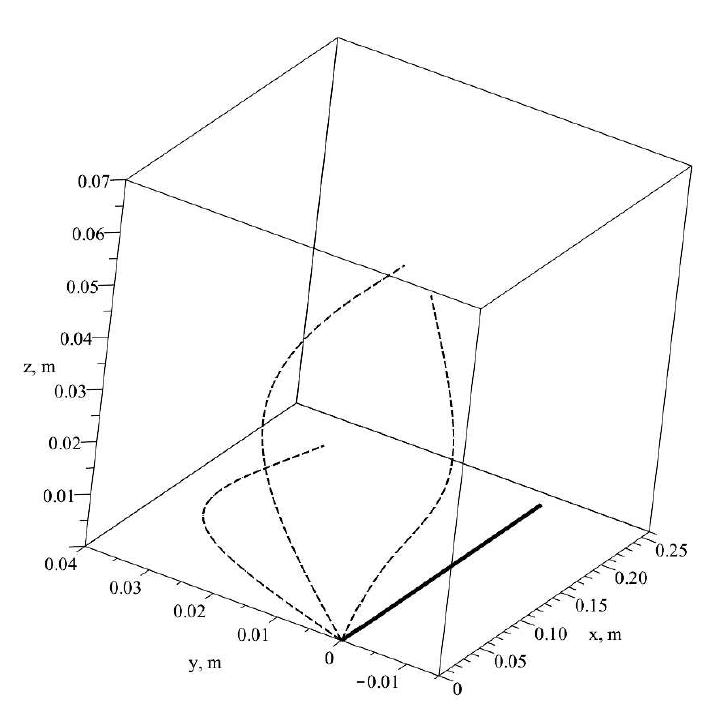
\includegraphics[width=0.5\linewidth]{Exp_BPR_1.png}
		\caption{Теоретическая (сплошная линия) и экспериментальные (штриховые линии) траектории движения безвинтового подводного робота при $\bK=(2i_1\omega_{max},  0,  0)$} 
		\label{traj1}
	\end{center}
\end{figure}

\textbf{2. Вращение одной пары малых роторов.} Траектория движения, полученная в результате численного моделирования при управляющих воздействиях, заданных в виде $\bK=\begin{pmatrix} 0,  2i_2\omega_{max}, 0 \end{pmatrix}$, и экспериментальная траектория движения, приведены на рисунке \ref{traj2}. После движения с заданными управляющими воздействиями в течение 3 секунд линейная и угловая скорость составили $\bV_t=\begin{pmatrix} 0, 0.0018, 0 \end{pmatrix}$ м/с, ${\bOm}_t=\begin{pmatrix} 0, 1.9436, 0 \end{pmatrix}$ об/мин. А изменение его ориентации  определяется углами: $\Delta \theta_t=35^{\circ}, \; \Delta \psi_t=0^{\circ}, \; \Delta \varphi_t=0^{\circ}$. При данном управляющем воздействии по результатам численного моделирования, робот проходит расстояние $|\br_t|=0.005$ м, а среднее значение перемещения по экспериментальным данным $|\br_{exp}|=0.087$ м.

\begin{figure}[h!]
	\begin{center}
		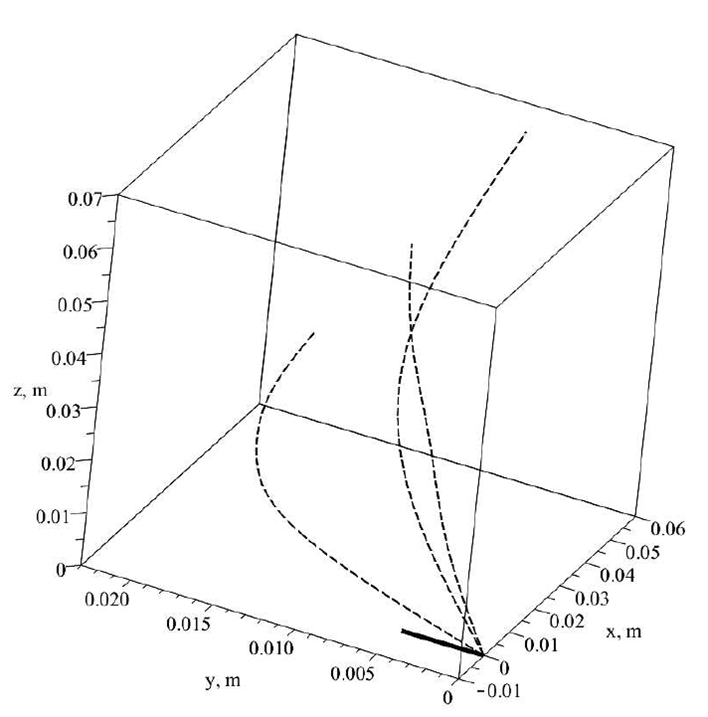
\includegraphics[width=0.5\linewidth]{Exp_BPR_2.png}
		\caption{Теоретическая (сплошная линия) и экспериментальные (штриховые линии) траектории движения безвинтового подводного робота при $\bK=( 0,  2i_2\omega_{max}, 0 )$} \label{traj2}
	\end{center}
\end{figure}

\textbf{3.	Вращение пары больших роторов и одной пары малых роторов.} Траектория движения, полученная в результате численного моделирования при управляющих воздействиях, заданных в виде $\bK=\begin{pmatrix} 2i_1\omega_{max}, 2i_2\omega_{max}, 0 \end{pmatrix}$, и экспериментальная траектория движения, приведены на рисунке \ref{traj3}. После движения с заданными управляющими воздействиями в течение 3 секунд линейная и угловая скорость составили $\bV_t=\begin{pmatrix} 0.0916,  0.0018, 0 \end{pmatrix}$ м/с, ${\bOm}_t=\begin{pmatrix} 41.0125, 1.9436, 0 \end{pmatrix}$ об/мин. А изменение его ориентации  определяется углами: $\Delta \theta_t=35^{\circ}, \; \Delta \psi_t=0^{\circ}, \; \Delta \varphi_t=738.2^{\circ}$. При данном управляющем воздействии по результатам численного моделирования, робот проходит расстояние $|\br_t|=0.275$ м, а среднее значение перемещения по экспериментальным данным $|\br_{exp}|=0.129$ м.

\begin{figure}[h!]
	\begin{center}
		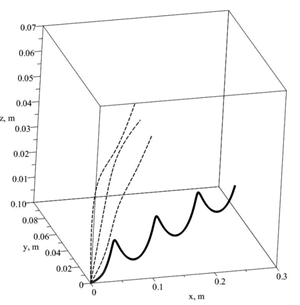
\includegraphics[width=0.5\linewidth]{Exp_BPR_3.png}
		\caption{Теоретическая (сплошная линия) и экспериментальные (штриховые линии) траектории движения безвинтового подводного робота $\bK=(2i_1\omega_{max}, 2i_2\omega_{max}, 0 )$} \label{traj3}
	\end{center}
\end{figure}

%\subsection{Выводы} при первых двух вариантах управляющих воздействий в рамках теоретической модели робот движется прямолинейно не изменяя своей ориентации. При проведении экспериментов такого движения добиться не удается.
Отметим, что при первых двух вариантах управляющих воздействий в рамках теоретической модели робот движется прямолинейно не изменяя своей ориентации. При проведении экспериментов такого движения добиться не удается. Так же перемещение безвинтового подводного робота на практике в два раза меньше, чем в теории. Более того в эксперименте при управляющем воздействии $\bK=\begin{pmatrix} 0,  2i_2\omega_{max}, 0 \end{pmatrix}$ движение робота происходит вдоль оси симметрии винтового тела (вдоль большей оси эллипсоида), а в теории робот движется перпендикулярно ей. Анализируя данные отклонения и характер движения безвинтового подводного робота в экспериментах, можно сделать следующие выводы:

\begin{enumerate}
	\item	Управляемое движение безвинтового подводного робота на практике продолжается до тех пор, пока обеспечивается ускоренное вращение роторов. Чем больше ускорение роторов, тем быстрее движется робот. Однако, технически, максимальная угловая скорость вращения роторов ограничена, и после ее достижения робот продолжает движение по инерции.
	\item Разгон маховиков до максимальной скорости занимает определенное время (разгон большего маховика --- $t=0.9$ секунды, разгон малого маховика --- $t=0.7$ секунды), что не учитывается в теоретической модели и вносит свой вклад в траекторию движения безвинтового подводного робота.
	\item	Движение безвинтового подводного робота сопровождается образованием вихревых структур, что подтверждается данными, полученными с использованием системы визуализации потоков (PIV --- Particle Image Velocimetry). На рисунке \ref{piv} изображены линии вихрей в вертикальной плоскости при движении эллипсоида в жидкости. Обеспечить безвихревое движение, как этого требует теория (см. \cite{Vetchanin_Mamaev_Tenenev_RCD_2013, Ramodanov_Tenenev_Treschev_RCD_2012}) с помощью роторов крайне затруднительно. Необходимо использовать модифицированные уравнения движения, учитывающие циркуляцию вокруг тела \cite{Kilin_Vetchanin_DAN_2016}.
	
	\begin{figure}[h!]
		\begin{center}
			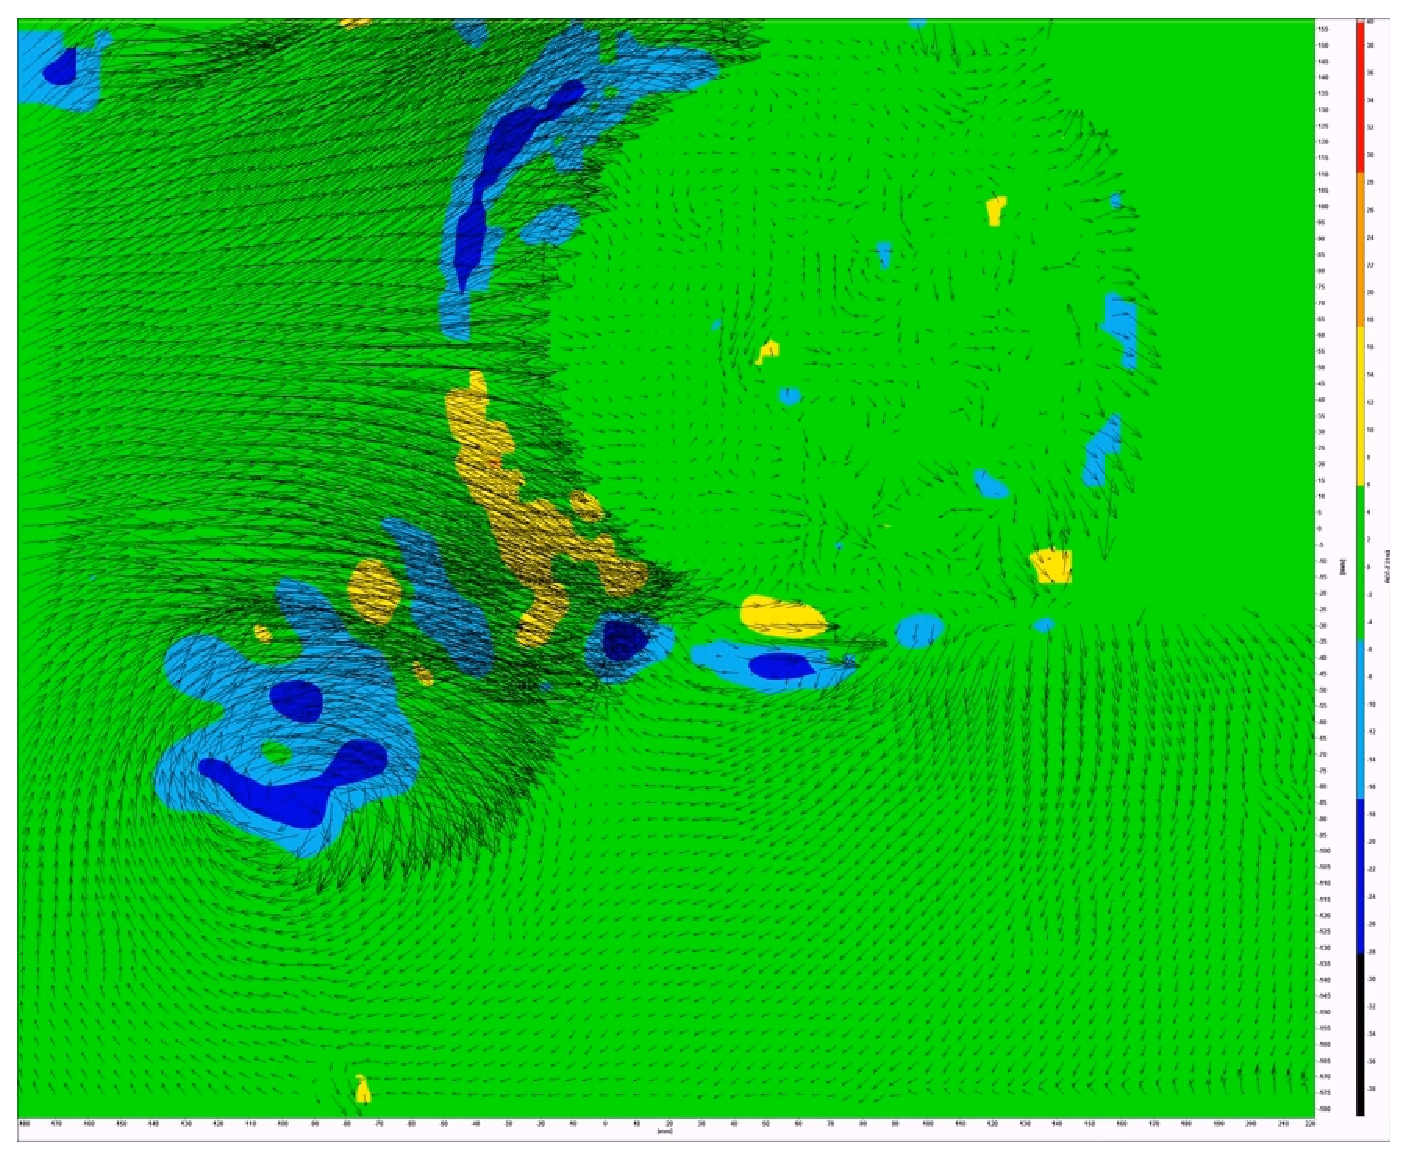
\includegraphics[width=0.4\linewidth]{piv.eps}
			\caption{Линии вихрей при движении эллипса в жидкости} \label{piv}
		\end{center}
	\end{figure}
	
	\item В теоретической модели используется идеализированная модель вязкости, что так же вносит несоответствия теоретической и реальной траектории движения.
	\item Подобную схему и алгоритмы управления в качестве практического применения можно использовать для реализации различных маневров (например, разворот на месте) в управлении подводными роботами.

\end{enumerate}


	
	
\clearpage           % Глава 4
\chapter*{Заключение}                       % Заголовок
\addcontentsline{toc}{chapter}{Заключение}  % Добавляем его в оглавление

%% Согласно ГОСТ Р 7.0.11-2011:
%% 5.3.3 В заключении диссертации излагают итоги выполненного исследования, рекомендации, перспективы дальнейшей разработки темы.
%% 9.2.3 В заключении автореферата диссертации излагают итоги данного исследования, рекомендации и перспективы дальнейшей разработки темы.
%% Поэтому имеет смысл сделать эту часть общей и загрузить из одного файла в автореферат и в диссертацию:

Основные результаты работы заключаются в следующем.
%% Согласно ГОСТ Р 7.0.11-2011:
%% 5.3.3 В заключении диссертации излагают итоги выполненного исследования, рекомендации, перспективы дальнейшей разработки темы.
%% 9.2.3 В заключении автореферата диссертации излагают итоги данного исследования, рекомендации и перспективы дальнейшей разработки темы.
\begin{enumerate}
  \item Разработана математическая модель движения безвинтового подводного робота в форме эллипсоида в жидкости за счет внутреннего гиростатического момента в рамках теории идеальной жидкости. Исследования управляемости модели показали, что для полной управляемости форму робота необходимо сделать винтовой.
  
  \item Разработаны конструкция и экспериментальный образец безвинтового подводного робота в форме эллипсоида. Учтено требование в необходимости винтовой формы робота, к оболочке в виде эллипсоида вращения добавлены винтовые лопасти. Проработана конструкция внутренних компонентов с учетом ограничений в размерах. Разработана система управления роботом.
  
  \item Проведены экспериментальные исследования безвинтового подводного робота в форме эллипсоида, проанализированы результаты. Для более точного описания движения необходимо учитывать в модели вязкое сопротивление, генерацию вихревых структур. В рамках дальнейшего исследования рассматривается движение объекта в форме симметричного профиля NACA 0040 по поверхности жидкости.
  
  \item Разработана математическая модель движения безвинтового надводного робота с оболочкой, имеющей форму симметричного профиля NACA 0040 и острую кромку, в жидкости за счет внутреннего гиростатического момента с учетом вязкого сопротивления. На основе анализа математической модели разработан алгоритм управления роботом, определена форма управляющего воздействия для движения вдоль прямой и вдоль окружности.
  
  \item Разработаны конструкция и экспериментальный образец безвинтового надводного робота с острой кромкой. Разработана система управления роботом.
  
  \item Проведены экспериментальные исследования с безвинтовым надводным роботом с острой кромкой, проанализированы результаты. Показано, что разработанная математическая модель качественно описывает движение робота. Рассмотрены движения вдоль прямой и вдоль окружности при различных управляющих воздействиях.
  
  \item По разработанным конструкциям получен патент на полезную модель безвинтового подводного робота в форме эллипсоида, для разработанных программных продуктов получены свидетельства о регистрации программ ЭВМ.
\end{enumerate}


\textbf{Участие в конференциях}
\begin{itemize}
	\item IV Всероссийская научно-техническая конференция аспирантов, магистрантов и молодых ученых с международным участием «Молодые ученые -- ускорению научно-технического прогресса в XXI веке». (Ижевск, 2016).
	\item Шестая международная конференция «Geometry, Dynamics, Integrable Systems -- GDIS 2016» (Ижевск, 2016 г.)
	\item Машиноведение и инновации. Конференция молодых учёных и студентов (МИКМУС-2018) (Москва, 2018 г.)
	\item International Conference "Scientific Heritage of Sergey A. Chaplygin: nonholonomic mechanics, vortex structures and hydrodynamics" (Чебоксары, 2019 г.)
	\item 30-я международная научно-техническая конференция "Экстремальная робототехника-2019" (Санкт-Петербург, 2019 г.)	
\end{itemize}

\textbf{Публикации}
\begin{itemize}
	
	\item Ветчанин Е. В, Караваев Ю.Л., Калинкин А.А., Пивоварова Е.Н., Клековкин А.В. Модель безвинтового подводного робота //Вестник Удмуртского университета. Математика. Механика. Компьютерные науки. – 2015. – Т. 25. – №. 4. – С. 544-553. (ВАК)
	
	\item Karavaev Y. L., Kilin A. A., Klekovkin A. V. Experimental investigations of the controlled motion of a screwless underwater robot // Regular and Chaotic Dynamics. – 2016. – Т. 21. – №. 7-8. – С. 918-926 (WoS)
	
	\item Klekovkin A.V., Karavaev Yu.L., Kilin A.A., Mamaev I.S. Control screwless fish-like robot with internal rotor // Extreme Robotics,  2019, Vol.1, no. 1, pp. 220-225 (РИНЦ)
	
	\item Karavaev Y.L., Klekovkin A.V., Mamaev I.S., Tenenev V.A., Vetchanin E.V. A Simple Physical Model for Control of an Propellerless Aquatic Robot. //  Mechanical Systems and Signal Processing, 2020, unpublished.
	
\end{itemize}



\textbf{Патенты}
\begin{itemize}

%	\item \todo{ № 2015615728. Программа для управления безвинтовым надводным роботом // А.В. Борисов, И.С. Мамаев, А.А. Килин, Ю.Л. Караваев, А.В. Клековкин, А.В. Шелухо, А.И. Кленов, Е.В. Ветчанин, В.А. Тененев. Заявитель и патентообладатель – ФБГОУ ВО «ИжГТУ имени М.Т. Калашникова»; Заявка: 2015612643, 07.04.2015, опубл. 22.05.2015}


\item Патент на полезную модель. №172254 РФ. Безвинтовой подводный робот //  А.В. Борисов, И.С. Мамаев, А.А. Килин, А.А. Калинкин, Ю.Л. Караваев, А.В. Клековкин, Е.В. Ветчанин; заявитель и патентообладатель – ФБГОУ ВО «ИжГТУ имени М.Т. Калашникова»; Заявка: 2016144812, 15.11.2016, опубл. 3.07.2017


\item № 2017613219. Программа для управления безвинтовым подводным роботом // А.В. Борисов, И.С. Мамаев, А.А. Килин, Ю.Л. Караваев, А.В. Клековкин. Заявитель и патентообладатель – ФБГОУ ВО «ИжГТУ имени М.Т. Калашникова»; Заявка: 2016662663, 22.11.2016, опубл. 16.03.2017


\item № 2019612284. Программа управления безвинтовым надводным роботом с внутренним ротором // А.В. Борисов, И.С. Мамаев, А.А. Килин, А.В. Клековкин, Ю.Л. Караваев. Заявитель и патентообладатель – ФБГОУ ВО "ИжГТУ имени М.Т. Калашникова"; Заявка: 2019610925, 04.02.2019, опубл. 14.02.2019


\end{itemize}


%И какая-нибудь заключающая фраза.

%Последний параграф может включать благодарности.  В заключение автор выражает благодарность и большую признательность научному руководителю Иванову~И.\:И. за поддержку, помощь, обсуждение результатов и~научное руководство. Также автор благодарит Сидорова~А.\:А. и~Петрова~Б.\:Б. за помощь в~работе с~образцами, Рабиновича~В.\:В. за предоставленные образцы и~обсуждение результатов, Занудятину~Г.\:Г. и авторов шаблона *Russian-Phd-LaTeX-Dissertation-Template* за~помощь в оформлении диссертации. Автор также благодарит много разных людей и~всех, кто сделал настоящую работу автора возможной.
      % Заключение
%\include{Dissertation/acronyms}        % Список сокращений и условных обозначений
%\include{Dissertation/dictionary}      % Словарь терминов
\clearpage                                  % В том числе гарантирует, что список литературы в оглавлении будет с правильным номером страницы
%\hypersetup{ urlcolor=black }               % Ссылки делаем чёрными
%\providecommand*{\BibDash}{}                % В стилях ugost2008 отключаем использование тире как разделителя
\urlstyle{rm}                               % ссылки URL обычным шрифтом
\ifdefmacro{\microtypesetup}{\microtypesetup{protrusion=false}}{} % не рекомендуется применять пакет микротипографики к автоматически генерируемому списку литературы
\insertbibliofull   
%\insertbiblioexternal                        % Подключаем Bib-базы
\ifdefmacro{\microtypesetup}{\microtypesetup{protrusion=true}}{}
\urlstyle{tt}                               % возвращаем установки шрифта ссылок URL
%\hypersetup{ urlcolor={urlcolor} }          % Восстанавливаем цвет ссылок      % Список литературы
%\include{Dissertation/lists}           % Списки таблиц и изображений (иллюстративный материал)

%%% Настройки для приложений
\appendix
% Оформление заголовков приложений ближе к ГОСТ:
\setlength{\midchapskip}{20pt}
\renewcommand*{\afterchapternum}{\par\nobreak\vskip \midchapskip}
\renewcommand\thechapter{\Asbuk{chapter}} % Чтобы приложения русскими буквами нумеровались

%%\begin{frame}
%    \frametitle{Ответы на замечания ведущей организации НИИ~<<Рога~и~копыта>>}
%    \begin{itemize}
%        \item Замечание -- ответ
%        \item Замечание -- ответ
%        \item Замечание -- ответ
%        \item Замечание -- ответ
%        \item Замечание -- ответ
%    \end{itemize}
%\end{frame}
%
%\begin{frame}
%    \frametitle{Ответы на замечания оф. оппонента Иванова\,И.\,И}
%    \begin{itemize}
%        \item Замечание -- ответ
%        \item Замечание -- ответ
%        \item Замечание -- ответ
%        \item Замечание -- ответ
%        \item Замечание -- ответ
%    \end{itemize}
%\end{frame}
%
%\begin{frame}
%    \frametitle{Ответы на замечания Петрова\,П.\,П}
%    \begin{itemize}
%        \item Замечание -- ответ
%        \item Замечание -- ответ
%        \item Замечание -- ответ
%        \item Замечание -- ответ
%        \item Замечание -- ответ
%    \end{itemize}
%\end{frame}

%\begin{frame}
%\frametitle{Участие в конференциях}
%\begin{itemize}
%	\item IV Всероссийская научно-техническая конференция аспирантов, магистрантов и молодых ученых с международным участием «Молодые ученые -- ускорению научно-технического прогресса в XXI веке». (Ижевск, 2016).
%	\item Шестая международная конференция «Geometry, Dynamics, Integrable Systems -- GDIS 2016» (Ижевск, 2016 г.)
%	\item Машиноведение и инновации. Конференция молодых учёных и студентов (МИКМУС-2018) (Москва, 2018 г.)
%	\item International Conference "Scientific Heritage of Sergey A. Chaplygin: nonholonomic mechanics, vortex structures and hydrodynamics" (Чебоксары, 2019 г.)
%	\item 30-я международная научно-техническая конференция "Экстремальная робототехника-2019" (Санкт-Петербург, 2019 г.)	
%	\item 23rd issue of the International Conference Series on Climbing and Walking Robots and the Support Technologies for Mobile Machines –- CLAWAR 2020 (Москва, 2020 г.)
%\end{itemize}
%\end{frame}
%
%\begin{frame}
%\frametitle{Публикации}
%%\textbf{Статьи}
%\begin{itemize}
%
%\item Ветчанин Е. В, Караваев Ю.Л., Калинкин А.А., Пивоварова Е.Н., Клековкин А.В. Модель безвинтового подводного робота //Вестник Удмуртского университета. Математика. Механика. Компьютерные науки. – 2015. – Т. 25. – №. 4. – С. 544-553. (ВАК)
%
%\item Karavaev Y. L., Kilin A. A., Klekovkin A. V. Experimental investigations of the controlled motion of a screwless underwater robot // Regular and Chaotic Dynamics. – 2016. – Т. 21. – №. 7-8. – С. 918-926 (WoS)
%
%\item Klekovkin A.V., Karavaev Yu.L., Kilin A.A., Mamaev I.S. Control screwless fish-like robot with internal rotor // Extreme Robotics,  2019, Vol.1, no. 1, pp. 220-225 (РИНЦ)
%
%\item Yury Karavaev, Anton Klekovkin, Ivan Mamaev, Valentin Tenenev, Eugene Vetchanin, "A Simple Physical Model for Control of an Propellerless Aquatic Robot",  Journal of Mechanisms and Robotics, 2020, unpublished. (WoS)
%
%
%\end{itemize}
%
%%\textbf{Патенты}
%%\begin{itemize}
%%	%	\item № 2015615728. Программа для управления безвинтовым надводным роботом // А.В. Борисов, И.С. Мамаев, А.А. Килин, Ю.Л. Караваев, А.В. Клековкин, А.В. Шелухо, А.И. Кленов, Е.В. Ветчанин, В.А. Тененев. Заявитель и патентообладатель – ФБГОУ ВО «ИжГТУ имени М.Т. Калашникова»; Заявка: 2015612643, 07.04.2015, опубл. 22.05.2015
%%		
%%	\item Патент на полезную модель. №172254 РФ. Безвинтовой подводный робот //  А.В. Борисов, И.С. Мамаев, А.А. Килин, А.А. Калинкин, Ю.Л. Караваев, А.В. Клековкин, Е.В. Ветчанин; %заявитель и патентообладатель – ФБГОУ ВО «ИжГТУ имени М.Т. Калашникова»; Заявка: 2016144812, 15.11.2016, опубл. 
%%	3.07.2017
%%		
%%	\item № 2017613219. Программа для управления безвинтовым подводным роботом // А.В. Борисов, И.С. Мамаев, А.А. Килин, Ю.Л. Караваев, А.В. Клековкин. %Заявитель и патентообладатель – ФБГОУ ВО «ИжГТУ имени М.Т. Калашникова»; Заявка: 2016662663, 22.11.2016, опубл. 
%%	16.03.2017
%%		
%%	\item № 2019612284. Программа управления безвинтовым надводным роботом с внутренним ротором // А.В. Борисов, И.С. Мамаев, А.А. Килин, А.В. Клековкин, Ю.Л. Караваев. %Заявитель и патентообладатель – ФБГОУ ВО "ИжГТУ имени М.Т. Калашникова"; Заявка: 2019610925, 04.02.2019, опубл. 
%%	14.02.2019
%%\end{itemize}
%
%\end{frame}
%
%\begin{frame}
%\frametitle{Патенты}
%\begin{itemize}
%
%%	\item № 2015615728. Программа для управления безвинтовым надводным роботом // А.В. Борисов, И.С. Мамаев, А.А. Килин, Ю.Л. Караваев, А.В. Клековкин, А.В. Шелухо, А.И. Кленов, Е.В. Ветчанин, В.А. Тененев. Заявитель и патентообладатель – ФБГОУ ВО «ИжГТУ имени М.Т. Калашникова»; Заявка: 2015612643, 07.04.2015, опубл. 22.05.2015
%
%
%\item Патент на полезную модель. №172254 РФ. Безвинтовой подводный робот //  А.В. Борисов, И.С. Мамаев, А.А. Килин, А.А. Калинкин, Ю.Л. Караваев, А.В. Клековкин, Е.В. Ветчанин; %заявитель и патентообладатель – ФБГОУ ВО «ИжГТУ имени М.Т. Калашникова»; Заявка: 2016144812, 15.11.2016, опубл. 
%3.07.2017
%
%
%\item № 2017613219. Программа для управления безвинтовым подводным роботом // А.В. Борисов, И.С. Мамаев, А.А. Килин, Ю.Л. Караваев, А.В. Клековкин. %Заявитель и патентообладатель – ФБГОУ ВО «ИжГТУ имени М.Т. Калашникова»; Заявка: 2016662663, 22.11.2016, опубл. 
%16.03.2017
%
%
%\item № 2019612284. Программа управления безвинтовым надводным роботом с внутренним ротором // А.В. Борисов, И.С. Мамаев, А.А. Килин, А.В. Клековкин, Ю.Л. Караваев. %Заявитель и патентообладатель – ФБГОУ ВО "ИжГТУ имени М.Т. Калашникова"; Заявка: 2019610925, 04.02.2019, опубл. 
%14.02.2019
%
%
%\end{itemize}
%\end{frame}

\begin{frame}
\frametitle{Кинетическая энергия}

\begin{minipage}{0.47\linewidth}
	Кинетическая энергия оболочки:
	\begin{gather}
	T_s = \frac{1}{2} m_s  \bigl( \bV,\, \bV \bigr) + \frac{1}{2} \bigl( {\bm I}_s {\bOm},\, {\bOm} \bigr),\nonumber
	\end{gather}
\end{minipage}
\hfill
\begin{minipage}{0.47\linewidth}
	Кинетическая энергия жидкости:
	\begin{gather}
	T_f = \frac{1}{2} \bigl( \bLam_1 \bV,\, \bV \bigr) + \frac{1}{2} \bigl( {\bLam} _2 {\bOm},\, {\bOm} \bigr).\nonumber
	\end{gather}
\end{minipage}

\vspace{2mm}

Кинетическая энергия $k$-го ротора:
\begin{gather}
T_k = \frac{1}{2} m_R \bigl( \bV + {\bOm} \times \br_k, \bV + {\bOm} \times \br_k \bigr) + \frac{1}{2}\Bigl({\bm I}_k \bigl( {\bOm} + \omega_k \bn_k \bigr), {\bOm} + \omega_k \bn_k \Bigr),\nonumber
\end{gather}

Суммарная кинетическая энергия всей системы: 		
\footnotesize
\begin{gather*}
\begin{split}
T = T_f + T_s + \sum _{k=1}^3 T_k = \frac{1}{2} \bigl( {\bbI} {\bOm},\, {\bOm} \bigr) + \bigl( {\bbB} {\bOm},\, \bV \bigr) + \frac{1}{2} \bigl( {\bbC} \bV,\, \bV \bigr) + \bigl( {\bOm},\, \bK(t) \bigr) + \frac{1}{2} \sum_{k=1}^3 i \omega_k^2 (t),
\end{split}
\end{gather*}

\small
Матрицы $\bbI$, $\bbB$, $\bbC$ имеют вид:	

\begin{minipage}{0.57\linewidth}
	\vspace{-3mm}
	\begin{gather}
	{\bbI} = {\bLam}_2 + {\bbI}_s + \sum _{k=1}^3 {\bbI}_k + \frac{1}{2} m_R \sum _{k=1}^3 \bigl( \br_k^2{\bbE} - \br_k \otimes \br_k \bigr),\nonumber \\
	{\bbC} = m {\bbE} + {\bLam}_1,\nonumber \quad	 m = m_s + 3 m_R		\nonumber
	\end{gather}
\end{minipage}
\hfill
\begin{minipage}{0.4\linewidth}
	\vspace{-3mm}
	\begin{gather}
	{\bbB} = m \begin{pmatrix}\nonumber
	0 & z_c & -y_c\\
	-z_c & 0 & x_c\\
	y_c & -x_c & 0
	\end{pmatrix}\nonumber	,	
	\end{gather}
\end{minipage}	

\vspace{2mm}

где $x_c$, $y_c$, $z_c$ --- компоненты радиус-вектора $\br_c$ центра масс системы. 

$\bK(t)=\sum \limits_{k=0}^3 i \omega_k (t)\bn_k$ --- вектор гиростатического момента. 


\end{frame}

\begin{frame}%[shrink=10]
\frametitle{Исследование управляемости системы}

Представим систему уравнений движения в виде
\begin{gather*}
\dot{\bq} = \bX_1 (\psi,\, \theta,\, \varphi) \Omega_1 + \bX_2 (\psi,\, \theta,\, \varphi) \Omega_2 + \bX_3 (\psi,\, \theta,\, \varphi) \Omega_3,
\end{gather*}
где $\bq = (x,\, y,\, z \, \psi,\, \theta,\, \varphi)$ -- вектор обобщенных координат.

\textbf{Теорема.} Система вида $\dot{\bq} = \sum_{i=1}^{M}\bX_i(\bq) u_i$, управляема в некоторой области $N$-мерного пространства, если среди векторных полей $\bX_i$ и всевозможных их коммутаторов $\bX_{i,j} = [\bX_i,\, \bX_j]$, $\bX_{k,(i,j)} = [\bX_k,\, \bX_{i,j}]$, \ldots, составленных последовательными применениями скобки Ли $[\cdot,\, \cdot]$, найдется $N$ линейно независимых в каждой точке области.\\

Построим следующие векторные поля:
\begin{gather*}
\begin{gathered}
\bX_{1,2} = \left[ \bX_1,\, \bX_2\right],\quad \bX_{3,1} = \left[ \bX_3,\, \bX_1\right],\quad \bX_{2,3} = \left[ \bX_2,\, \bX_3\right], \\  
\bX_{1,(2,3)} = \left[ \bX_1,\, \bX_{2,3}\right],\quad \bX_{2,(3,1)} = \left[ \bX_2,\, \bX_{3,1}\right], \quad \bX_{3,(1,2)} = \left[ \bX_3,\, \bX_{1,2}\right],\\
\end{gathered}
\end{gather*}
Выберем три набора векторных полей
\begin{gather*}
\begin{gathered}
\Bigl( \bX_1,\, \bX_2,\,\bX_3,\,\bX_{1,2},\,\bX_{2,3},\,\bX_{2,(3,1)},\, \Bigr),\quad
\Bigl( \bX_1,\, \bX_2,\,\bX_3,\,\bX_{2,3},\,\bX_{3,1},\,\bX_{3,(1,2)},\, \Bigr), \\
\Bigl( \bX_1,\, \bX_2,\,\bX_3,\,\bX_{3,1},\,\bX_{1,2},\,\bX_{1,(2,3)},\, \Bigr),
\end{gathered}
\end{gather*}


Скобка Ли для векторных полей $ \bbs v $ и $ \bbs u $ имеет выражение
\begin{gather*}
[\bbs v, \bbs u]_{i}=\sum_{j}v_{j}\frac{\partial u_{i}}{\partial q_{j}}-u_{j}\frac{\partial v_{i}}{\partial q_{j}}
\end{gather*}


\end{frame}


\begin{frame}
\frametitle{Исследование управляемости системы}

Условия линейной зависимости векторных полей в указанных наборах имеют вид
\begin{gather*}
\begin{gathered}
x_c(c_2 - c_3) = 0,\quad
y_c(c_3-c_1) = 0, \quad
z_c(c_1-c_2) = 0.
\end{gathered}
\end{gather*}

Движение в идеальной жидкости однородной оболочки, имеющей форму эллипсоида, вполне управляемо с помощью вращения трех роторов, за исключением трех частных случаев:
\begin{enumerate}
	\item система “ оболочка + роторы” уравновешена;
	\item оболочка имеет сферическую форму;
	\item оболочка имеет форму эллипсоида вращения, а центра масс всей системы	расположен на оси вращения.
\end{enumerate}

Добавим к оболочке в виде эллипсоида винтовые лопасти. Так, объект будет представлять из себя трехлопастной винт.

\end{frame}

\begin{frame}
\frametitle{Результаты моделирования}
%\begin{itemize}
%	\item Борисов А. В., Ветчанин Е. В., Килин А. А., Управление движением трехосного эллипсоида в жидкости с помощью роторов, Математические заметки, 2017, т. 102, № 4, с. 503-513
%	\item В работе описаны комбинации управляющих воздействий, которые позволяют реализовать неограниченное движение в произвольном направлении.
%	
%	Движение тела представляет собой стационарное винтовое движение с постоянной угловой и линейной скоростями. 
%\end{itemize}


Для решения уравнений движения необходимо:
\begin{itemize}
	\item Определить значения тензоров присоединенных масс и присоединенных моментов инерции. 
	%Для робота в форме эллипсоида вращения данные коэффициенты можно расчитать используя справочные материалы.
	Для робота винтовой формы коэффициенты расчитывались с помощью программных продуктов SALOME (генерация сетки) и OpenFOAM (численные расчеты).
	\item Определить значения моментов инерции. Для робота разработанной конструкции моменты инерции определялись с помощью программного продукта SolidWorks.	
\end{itemize}

Рассмотрим движение тела при постоянных скоростях вращения роторов $\bbs\omega = (\omega_1, \omega_2, \omega_3)^T$.

а) $\omega_1=10$ рад/с, $\omega_2=0$, $\omega_3=0$. б) $\omega_1=0$, $\omega_2=10$ рад/с, $\omega_3=0$. 

в) $\omega_1=10$ рад/с, $\omega_2=10$ рад/с, $\omega_3=0$.

\begin{minipage}[t]{0.3\linewidth}
	\center{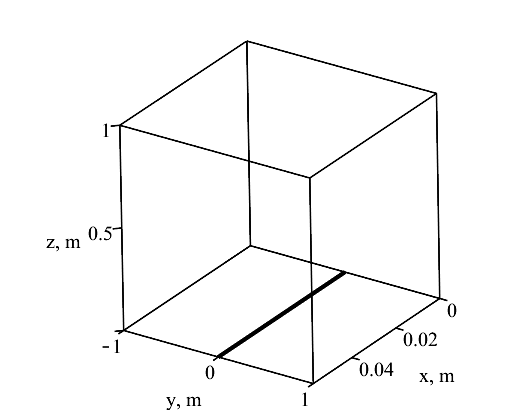
\includegraphics[width=0.95\linewidth]{ModelTrBPR1_.png} \\ а)}
\end{minipage}
\hfill
\begin{minipage}[t]{0.3\linewidth}
	\center{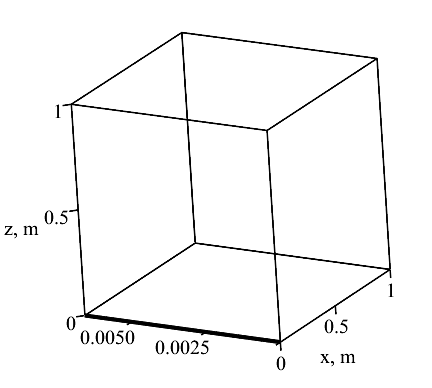
\includegraphics[width=0.95\linewidth]{ModelTrBPR2_.png} \\ б)}
\end{minipage}
\hfill
\begin{minipage}[t]{0.3\linewidth}
	\center{\includegraphics[width=1\linewidth]{ModelTrBPR12_.png} \\ в)}
\end{minipage}


\end{frame}

\begin{frame}
\frametitle{Экспериментальные исследования}
1.	Вращение пары больших роторов. $K = (2i_1\omega_{max}, 0, 0)$.


	\begin{minipage}[t]{0.3\linewidth}
		\center{\includegraphics[width=0.7\linewidth]{exp11.eps} \\ а)}
	\end{minipage}
	\hfill
	\begin{minipage}[t]{0.3\linewidth}
		\center{\includegraphics[width=0.7\linewidth]{exp12.eps} \\ б)}
	\end{minipage}
	\hfill
	\begin{minipage}[t]{0.3\linewidth}
		\center{\includegraphics[width=0.8\linewidth]{Exp_BPR_1.png} \\ в)}
	\end{minipage}


Положение робота а) в начальный момент времени и б) момент времени t=3 секунды от начала движения; в) теоретическая (сплошная линия) и экспериментальные (штриховые линии) траектории движения безвинтового подводного робота 

\begin{table}[h]
	\centering
	\begin{tabular}{|c|c|c|c|c|c|c|c|}
		\hline
		& $\Delta x$, м & $\Delta y$, м & $\Delta z$, м & $|\br_t|$, м & $\Delta \theta$ & $\Delta \psi$ & $\Delta \varphi$ \\ \hline
		Теория & $0.275$ & $0$ & $0$ & $0.275$ & $ 0^{\circ}$ & $ 0^{\circ}$ & $ 738.2^{\circ}$ \\ \hline
		Эксперимент & $0.115$  & $0.010$ & $0.055$ & $0.128$ & $ 4^{\circ} $ & $ 10^{\circ} $ & $ 121^{\circ} $  \\
		\hline
	\end{tabular}
\end{table}

\end{frame}


\begin{frame}
\frametitle{Экспериментальные исследования}
2.	Вращение одной пары малых роторов. $K = (0, 2i_2\omega_{max}, 0)$. 


	\begin{minipage}[h]{0.3\linewidth}
		\center{\includegraphics[width=0.7\linewidth]{exp21.eps} \\ а)}
	\end{minipage}
	\hfill
	\begin{minipage}[h]{0.3\linewidth}
		\center{\includegraphics[width=0.7\linewidth]{exp22.eps} \\ б)}
	\end{minipage}
	\hfill
	\begin{minipage}[h]{0.3\linewidth}
		\center{\includegraphics[width=0.8\linewidth]{Exp_BPR_2.png} \\ в)}
	\end{minipage}


Положение робота а) в начальный момент времени и б) момент времени t=3 секунды от начала движения; в) теоретическая (сплошная линия) и экспериментальные (штриховые линии) траектории движения безвинтового подводного робота 

\begin{table}[h]
	\centering
	\begin{tabular}{|c|c|c|c|c|c|c|c|}
		\hline
		& $\Delta x$, м & $\Delta y$, м & $\Delta z$, м & $|\br_t|$, м & $\Delta \theta$ & $\Delta \psi$ & $\Delta \varphi$ \\ \hline
		Теория & $0$ & $0.005$ & $0$ & $0.005$ & $ 35^{\circ}$ & $ 0^{\circ}$ & $ 0^{\circ}$ \\ \hline
		Эксперимент & $0.054$  & $0.008$ & $0.068$ & $0.087$ & $ 61^{\circ} $ & $ 62^{\circ} $ & $ 10^{\circ} $  \\
		\hline
	\end{tabular}
\end{table}

\end{frame}


\begin{frame}
\frametitle{Экспериментальные исследования}
3.	Вращение пары больших роторов и одной пары малых роторов. $K = (2i_1\omega_{max}, 2i_2\omega_{max}, 0)$. 

	\begin{minipage}[h]{0.3\linewidth}
		\center{\includegraphics[width=0.7\linewidth]{exp31.eps} \\ а)}
	\end{minipage}
	\hfill
	\begin{minipage}[h]{0.3\linewidth}
		\center{\includegraphics[width=0.7\linewidth]{exp32.eps} \\ б)}
	\end{minipage}
	\hfill
	\begin{minipage}[h]{0.3\linewidth}
		\center{\includegraphics[width=0.8\linewidth]{Exp_BPR_3.png} \\ в)}
	\end{minipage}

Положение робота а) в начальный момент времени и б) момент времени t=3 секунды от начала движения; в) теоретическая (сплошная линия) и экспериментальные (штриховые линии) траектории движения безвинтового подводного робота 

\begin{table}[h]
	\centering
	\begin{tabular}{|c|c|c|c|c|c|c|c|}
		\hline
		& $\Delta x$, м & $\Delta y$, м & $\Delta z$, м & $|\br_t|$, м & $\Delta \theta$ & $\Delta \psi$ & $\Delta \varphi$ \\ \hline
		Теория & $0.275$ & $0$ & $0$ & $0.275$ & $ 35^{\circ}$ & $ 0^{\circ}$ & $ 738.2^{\circ}$ \\ \hline
		Эксперимент & $0.106$  & $0.050$ & $0.053$ & $0.189$ & $ 17^{\circ} $ & $ 92^{\circ} $ & $ 51^{\circ} $  \\
		\hline
	\end{tabular}
\end{table}

%\begin{center}
%	$\Delta x_{exp}=0.106\; \mbox{м}, \; \Delta y_{exp}=0.050\; \mbox{м},\; \Delta z_{exp}=0.053\; \mbox{м}, \;$ \\
%	%\item $|r|=0.129$ м;
%	$\Delta \theta_{exp}=17^{\circ},\; \Delta \psi_{exp}=90^{\circ},\; \Delta \varphi_{exp}=51^{\circ}.$
%\end{center}

\end{frame}

\begin{frame}
\frametitle{Закон изменения угловой скорости ротора}

	В общем случае, зависимость угловой скорости ротора от времени будет иметь характерные переходные интервалы, соответствующие разгону и торможению 
	
		\scriptsize 
		\vspace{-4mm}
		\begin{equation*}
		\omega_r(t) =
		\begin{cases}
		
		\omega_1 & t \in \left[ nT;  nT + t_1 \right] ,\\
		
		\frac{(\omega_2 - \omega_1)(t-nT)}{t_2} - \frac{(\omega_2 - \omega_1)(t_1+t_2)}{t_2} + \omega_2 & t \in \left[ nT + t_1;  nT + t_1+t_2 \right], \\
		
		\omega_2 & t \in \left[ nT + t_1+t_2;  nT + t_1+t_2+t_3 \right] ,\\
		
		\frac{(\omega_1 - \omega_2)(t-nT)}{t_4} - \frac{(\omega_1 - \omega_2)(t_1+t_2+t_3+t_4)}{t_4} + \omega_1 &t \in \left[ nT + t_1 + t_2+t_3;  nT + t_1+t_2+t_3+t_4 \right] ,
		
		\end{cases}
		\label{omegaRotorGeneral}
		\end{equation*}
		
		\small
		где $n \in \mathbf{N}$, $T$ -- период управляющего воздействия; $ \omega_1, \omega_2 $ -- амплитуды угловой скорости вращения ротора по часовой стрелке и против часовой стрелки соответственно; $t_1, t_2, t_3, t_4$ -- задают продолжительность по времени характерных интервалов угловой скорости вращения ротора. 
		
			%\framebreak
		
		%Графически данная зависимость приведена на рисунке
		
		\begin{minipage}[t]{0.47\linewidth}
			\begin{figure}[!ht]
				\centering
				\includegraphics[height=33mm]{ControlAction.eps}
			\end{figure}
			
		\end{minipage}	
		\hfill
		\begin{minipage}[t]{0.47\linewidth}
			\begin{figure}[!ht]
				\centering
				\includegraphics[height=33mm]{ControlActionEpsilon.eps}
			\end{figure}
		\end{minipage}	
%		\begin{figure}[!ht]
%			\centering
%			\includegraphics[width=0.4\linewidth]{ControlAction.eps}
%		\end{figure}
	
	
\end{frame}

\begin{frame}
\frametitle{Методика определения коэффициентов}

Уравнения Навье-Стокса, записанные относительно криволинейной системы координат $(\xi,\, \eta)$, связанной с движущимся профилем имеют вид:
\begin{gather*}
\begin{gathered}
\pder{Du_1}{\xi} + \pder{Du_2}{\eta} = 0,\\
\begin{split}
\pder{u_1}{t} + \frac{1}{D^2} \biggl( \pder{D(u_1 - w_1)u_1}{\xi} + & \pder{D(u_2 - w_2)u_1}{\eta} \biggr) = \\
= - \frac{1}{D\rho} \pder{p}{\xi} + & \frac{\nu}{D^2} \left( \pdder{u_1}{\xi}{2} + \pdder{u_1}{\eta}{2} \right) + \beta_1 + 2 u_2 \omega
\end{split}\\
\begin{split}
\pder{u_2}{t} + \frac{1}{D^2} \biggl( \pder{D(u_1 - w_1)u_2}{\xi} + & \pder{D(u_2 - w_2)u_2}{\eta} \biggr) = \\
= - \frac{1}{D\rho} \pder{p}{\eta} + & \frac{1}{D^2} \left( \pdder{u_2}{\xi}{2} + \pdder{u_2}{\eta}{2} \right) + \beta_2 - 2 u_1 \omega,
\end{split}
\end{gathered}
\end{gather*}
где $u_1$, $u_2$ --- проекции вектора скорости жидкости на криволинейные оси, $p$ --- давление, $\rho$ --- плотность жидкости, $\nu$ --- кинематическая вязкость, $w_1 = v_1 - \omega x_2(\xi,\, \eta)$, $w_2 = v_2 + \omega x_1(\xi,\, \eta)$ --- компоненты переносной скорости. 

\end{frame}

\begin{frame}
\frametitle{Методика определения коэффициентов}


Коэффициент Ламэ $D$ и члены $\beta_1$, $\beta_2$, возникающие вследствие искривления сеточных линий, имеют вид:
\begin{gather*}
D = \sqrt{\left( \pder{x_1}{\xi}\right)^2 + \left( \pder{x_2}{\xi}\right)^2  } =\sqrt{\left( \pder{x_1}{\eta}\right)^2 + \left( \pder{x_2}{\eta}\right)^2  },\\
\begin{split}
\beta_1 = \frac{\nu}{D^3} \Biggl( u_1\left( \pdder{D}{\xi}{2} + \pdder{D}{\eta}{2} \right) + {} & {} 2 \pder{u_1}{\xi} \pder{D}{\xi} + 2 \pder{u_2}{\xi} \pder{D}{\eta} + \\
+ {} & {} \frac{2u_2}{D} \pder{D}{\xi} \pder{D}{\eta} - \frac{2u_1}{D} \left( \pder{D}{\eta} \right)^2  \Biggr)
\end{split}\\
\begin{split}
\beta_2 = \frac{\nu}{D^3} \Biggl( u_2\left( \pdder{D}{\xi}{2} + \pdder{D}{\eta}{2} \right) + {} & {} 2 \pder{u_1}{\eta} \pder{D}{\xi} + 2 \pder{u_2}{\eta} \pder{D}{\eta} + \\
+ {} & {} \frac{2u_1}{D} \pder{D}{\xi} \pder{D}{\eta} - \frac{2u_2}{D} \left( \pder{D}{\xi}\right)^2 \Biggr)
\end{split}
\end{gather*}

\end{frame}




\begin{frame}
\frametitle{Методика определения коэффициентов}

При известных распределениях $u_1$, $u_2$, $p$ cилы $f_1$, $f_2$ и момент $g$, действующие на тело со стороны жидкости, определяются следующими интегралами по контуру $L$ профиля:
\begin{gather*}
\begin{gathered}
f_1 = \oint_L \left( p \pder{x_2}{\xi} + \frac{\rho \nu}{D} \pder{u_1}{\eta} \pder{x_1}{\xi} \right) d\xi,\\
f_2 = \oint_L \left( -p \pder{x_1}{\xi} + \frac{\rho \nu}{D} \pder{u_1}{\eta} \pder{x_2}{\xi} \right) d\xi,\\
g = \oint_L \left( x_1 \left( -p \pder{x_1}{\xi} + \frac{\rho \nu}{D} \pder{u_1}{\eta} \pder{x_2}{\xi} \right) - x_2 \left( p \pder{x_2}{\xi} + \frac{\rho \nu}{D} \pder{u_1}{\eta} \pder{x_1}{\xi} \right) \right) d\xi - \dot{k}(t).
\end{gathered}\label{eq.fgNS}
\end{gather*}

Поскольку движение робота является существенно нестационарным, оказывается невозможным определение коэффициентов $\lambda_{11}$, $\lambda_{22}$, $\lambda_{33}$, $\lambda_{23}$, $c_1$, $c_2$, $c_3$ по-отдельности. Таким образом данные коэффициенты должны определяться совместно с учетом нестационарности движение профиля.

%	Для задания граничных условий, соответствующих нестационарному движению профиля, будем использовать экспериментальные данные для прототипа, описанного в разделе 1 с периодом управляющего воздействия $T = 1$ с, которые представляют собой таблицу значений:
%	\begin{gather}
%	(t_i,\, x_i,\, y_i,\, \alpha_i),\quad i = 0,\, \ldots,\, N.\label{eq.expXYPhi}
%	\end{gather}
%	Здесь $t_i$ --- момент времени, $(x_i,\, y_i)$ --- положение центра масс профиля в момент времени $t_i$, $\alpha_i$ --- ориентация профиля в момент времени $t_i$.
%	
\begin{gather*}
\begin{gathered}
\lambda_{11}^{(1)} \approx 0.3087, \quad 
\lambda_{22}^{(1)} \approx -0.5796,\quad 
\lambda_{23}^{(1)} \approx 0.039085,\\
\lambda_{22}^{(2)} \approx 2.0996,\quad 
\lambda_{23}^{(2)} \approx 0.17629,\quad
\lambda_{11}^{(2)} \approx -7.9826,\\
\lambda_{23,l}^{(3)} \approx 0.083474,\quad
\lambda_{33}^{(2)} \approx 0.018935,\quad
\lambda_{11}^{(3)} - \lambda_{22}^{(3)} \approx - 4.7550,\quad
\lambda_{23,r}^{(3)} \approx 1.4488,\\
c_1 = 0.04715,\quad c_2 = 17.702,\quad c_3 = 0.092872.
\end{gathered}\label{eq.coeffs2}
\end{gather*}


\end{frame}        % Приложения

\end{document}
